%%%%%%%%%%%%%%%%%%%%%%%%%%%%%%%%%%%%%%%%%
%This documentclass loads the packages  %
%            setspace                   %
% and                                   %
%           fancyhdr.                   %
%You may have to                        %
%get these if your TeX distribution     %
%doesn't have them.                     %
%%%%%%%%%%%%%%%%%%%%%%%%%%%%%%%%%%%%%%%%%
\documentclass{aux/ttuthes2007}

%%%%%%%%%%%%%%%%%%%%%%%%%%%%%%%%%%%%%%%%%%%%%%
%Include any other add-on  packages you need:%
%%%%%%%%%%%%%%%%%%%%%%%%%%%%%%%%%%%%%%%%%%%%%%
\usepackage{amsmath,graphicx,bm,mathtools, amssymb}
\allowdisplaybreaks
\usepackage{booktabs} % Required for better horizontal rules in tables
\usepackage{listings} % Required for insertion of code
\usepackage[utf8]{inputenc}
\usepackage[T1]{fontenc}
\usepackage{lmodern}
\usepackage[labelfont=bf,labelsep=period]{caption}
\usepackage{multirow}
\usepackage{textcomp}
\usepackage[colorlinks=true,citecolor=black,linkcolor=black]{hyperref}
\usepackage{afterpage}
\usepackage{pdflscape}
\usepackage{hhline}
\usepackage{enumitem}
\usepackage{hyperref}
\usepackage{bm}
\usepackage[acronyms,toc,nonumberlist,nogroupskip]{glossaries}
\usepackage{datetime}
\usepackage{xstring} % conditionals
\usepackage[dvipsnames]{xcolor}

\newglossary{symbols}{sym}{sbl}{List of Symbols}
\makenoidxglossaries
\glsnoexpandfields

\loadglsentries{aux/gloss.tex}

%%%%%%%%%%%%%%%%%%%%%%%%%%%%%%%%%%
%EDIT  (Running head--  REQUIRED)%
%%%%%%%%%%%%%%%%%%%%%%%%%%%%%%%%%%
\rhead{\small Texas Tech University, \textit{Lucas Ramos Cardoso Tin\^{o}co Cortez}, \monthyeardate\today}	%update your name and graduation date-year here

%%%%%%%%%%%%%%%%%%%%%%%%%%%%%%%%%%%%%%%%%%%%%%%
%Uncomment if the grad school doesn't like the%
%line under the  running head:                %
%%%%%%%%%%%%%%%%%%%%%%%%%%%%%%%%%%%%%%%%%%%%%%%
%\renewcommand{\headrulewidth}{0pt}


%%%%%%%%%%%%%%%%%%%%%%%%%%%%%%%%%%%%%%%%%%%%%%%%%%
%Spacing -- Do you want double or one-and-a-half?%
%%%%%%%%%%%%%%%%%%%%%%%%%%%%%%%%%%%%%%%%%%%%%%%%%%
%\doublespacing
\onehalfspacing
%%%%%%%%%%%%%%%%%%%%%%%%%%%%%%%%%%%%%%%%%%%%%%%%%%%%%%%%%%%%%
%Leave the one you want uncommented.                        %
%In places where single-line-spacing is appropriate         %
%e.g, extended quotations, you can enclose the material     %
%in a singlespacing environment (with \begin{singlespacing} %
% ...  \end{singlespacing}                                  %
%%%%%%%%%%%%%%%%%%%%%%%%%%%%%%%%%%%%%%%%%%%%%%%%%%%%%%%%%%%%%


%%%%%%%%%%%%%%%%%%%%%%%%%%%%%%%%%%%%%%%%%%%%%%%%%%
%Other preamble stuff, e.g., theorem environments%
%or newcommands go here:                         %
% e.g.                                           %
%%%%%%%%%%%%%%%%%%%%%%%%%%%%%%%%%%%%%%%%%%%%%%%%%%
% \newtheorem{theorem}{Theorem}
% \newtheorem{proposition}[theorem]{proposition}
% \newtheorem{question}{Question}
% \newtheorem{conjecture}{Conjecture}
%\newcommand\Set[2]{\left\{\,#1\middle\mid#2\,\right\}}
\newcommand{\bx}{\bm{x}}
\newcommand{\br}{\bm{r}}
\newcommand{\bra}[1]{\ensuremath{\left\langle#1\right\vert}}
\newcommand{\ket}[1]{\ensuremath{\left|#1\right\rangle}}
\newcommand{\braket}[2]{\left< #1 \middle\vert #2 \right>}
\newcommand{\sandwich}[3]{\left< #1 \middle\vert #2 \middle\vert #3 \right>}
%\newcommand{\norm}[1]{\left\lVert #1 \right\rVert}
%\newcommand{\abs}[1]{\lVert #1 \rVert}
\newcommand{\inpr}[1]{\left< #1 \right>}
\newcommand{\s}[1]{\sin\left( #1 \right)}
\newcommand{\ssq}[1]{\sin^2\left( #1 \right)}
\newcommand{\co}[1]{\cos\left( #1 \right)}
\newcommand{\cosq}[1]{\cos^2\left( #1 \right)}
\newcommand{\av}[1]{\left< #1 \right>}
\newcommand{\her}[2]{H_{#1}\left( #2 \right)}
\newcommand{\herv}[1]{H_{\nu}\left( #1 \right)}
\renewcommand{\labelenumi}{\Roman{enumi} -}
\newcommand{\ex}[1]{\exp\left( #1 \right)}
\newcommand{\closepar}{)}
\newcommand{\paren}[1]{\left( #1 \right)}
\newcommand{\ddx}{\frac{d}{dx}}
\newcommand{\ddt}{\frac{d}{dt}}
\newcommand{\pdx}{\frac{\partial}{\partial x}}
\newcommand{\pdt}{\frac{\partial}{\partial t}}
\newcommand{\dd}[1]{\frac{d}{d#1}}
\newcommand{\pd}[1]{\frac{\partial}{\partial #1}}
\newcommand{\fpd}[2]{\frac{\partial #1}{\partial #2}}
\newcommand{\pp}[1]{\frac{\partial \Psi}{\partial #1}}
\newcommand{\kpp}[1]{\frac{\partial \ket\Psi}{\partial #1}}
\newcommand{\bpp}[1]{\frac{\partial \bra\Psi}{\partial #1}}
\newcommand{\kppn}[2]{\frac{\partial^{#2} \ket\Psi}{\partial {#1}^{#2}}}
\newcommand{\bppn}[2]{\frac{\partial^{#2} \bra\Psi}{\partial {#1}^{#2}}}
\newcommand{\kppd}[2]{\frac{\partial^{2} \ket\Psi}{\partial #1 \partial #2}}
\newcommand{\bppd}[2]{\frac{\partial^{2} \bra\Psi}{\partial #1 \partial #2}}
\newcommand{\ddn}[2]{\frac{d^{#1}}{d#2^{#1}}}
\newcommand{\pdn}[2]{\frac{\partial^{#1}}{\partial#2^{#1}}}
%\newcommand{\orb}{N}
%\newcommand{\elec}{n}
\newcommand{\elec}{N}
\newcommand{\nuc}{N_{N}}
\newcommand{\orb}{K}
\newcommand{\Ld}[1]{\hat L_{#1}}
\newcommand{\anio}[1]{a_{\oo{#1}}}
\newcommand{\aniu}[1]{a_{\uo{#1}}}
\newcommand{\anig}[1]{a_{\go{#1}}}
\newcommand{\creo}[1]{a^\dagger_{\oo{#1}}}
\newcommand{\creu}[1]{a^\dagger_{\uo{#1}}}
\newcommand{\creg}[1]{a^\dagger_{\go{#1}}}
\newcommand{\vac}{\ket{vac}}
\newcommand{\anticom}[2]{\left\{ #1, #2 \right\}}
\newcommand{\ind}[1]{{\uo #1 \oo #1}}

\newcommand{\rmatdd}[1]{
		\IfEqCase{#1}{
			{6}{\ensuremath{
	\begin{bmatrix}
		e^{\frac{-i \omega_\ind 0} 2 } & 0 & 0 & 0 \\
		0 & e^{\frac{-i \omega_\ind 0} 2 } & 0 & 0 \\
		0 & 0 & e^{\frac{i \omega_\ind 0} 2 } & 0 \\
		0 & 0 & 0 & e^{\frac{i \omega_\ind 0} 2 }
	\end{bmatrix}
}}
			{5}{\ensuremath{
	\begin{bmatrix}
		e^{\frac{-i \omega_\ind 1} 2 } & 0 & 0 & 0 \\
		0 & e^{\frac{i \omega_\ind 1} 2 } & 0 & 0 \\
		0 & 0 & e^{\frac{-i \omega_\ind 1} 2 } & 0 \\
		0 & 0 & 0 & e^{\frac{i \omega_\ind 1} 2 }
	\end{bmatrix} 
}}
			{4}{\ensuremath{
	\begin{bmatrix}
		\cos\left(\rho_\ind 0\right) & 0 & \sin\left(\rho_\ind 0\right) & 0 \\
		0 & \cos\left(\rho_\ind 0\right) & 0 & -\sin\left(\rho_\ind 0\right) \\
		\sin\left(\rho_\ind 0\right) & 0 & -\cos\left(\rho_\ind 0\right) & 0 \\
		0 & \sin\left(\rho_\ind 0\right) & 0 & \cos\left(\rho_\ind 0\right)
	\end{bmatrix}
}}
			{3}{\ensuremath{
	\begin{bmatrix}
		\cos\left(\rho_\ind 1\right) & -\sin\left(\rho_\ind 1\right) & 0 & 0 \\
		\sin\left(\rho_\ind 1\right) & \cos\left(\rho_\ind 1\right) & 0 & 0 \\
		0 & 0 & -\cos\left(\rho_\ind 1\right) & \sin\left(\rho_\ind 1\right) \\
		0 & 0 & \sin\left(\rho_\ind 1\right) & \cos\left(\rho_\ind 1\right)
	\end{bmatrix}
}}
			{2}{\ensuremath{
	\begin{bmatrix}
		e^{\frac{i \omega_\ind 0} 2 } & 0 & 0 & 0 \\
		0 & e^{\frac{i \omega_\ind 0} 2 } & 0 & 0 \\
		0 & 0 & e^{\frac{-i \omega_\ind 0} 2 } & 0 \\
		0 & 0 & 0 & e^{\frac{-i \omega_\ind 0} 2 }
	\end{bmatrix}
}}
			{1}{\ensuremath{
	\begin{bmatrix}
		e^{\frac{i \omega_\ind 1} 2 } & 0 & 0 & 0 \\
		0 & e^{\frac{-i \omega_\ind 1} 2 } & 0 & 0 \\
		0 & 0 & e^{\frac{i \omega_\ind 1} 2 } & 0 \\
		0 & 0 & 0 & e^{\frac{-i \omega_\ind 1} 2 }
	\end{bmatrix}
}}
		}[\PackageError{r2d}{Undefined option to rmat: #1}{}]
}

\newcommand{\paulid}[1]{
		\IfEqCase{#1}{
			{ii}{\bm I \otimes \bm I}
			{ix}{\bm I \otimes \bm X}
			{iy}{\bm I \otimes \bm Y}
			{iz}{\bm I \otimes \bm Z}
			{xi}{\bm X \otimes \bm I}
			{xx}{\bm X \otimes \bm X}
			{xy}{\bm X \otimes \bm Y}
			{xz}{\bm X \otimes \bm Z}
			{yi}{\bm Y \otimes \bm I}
			{yx}{\bm Y \otimes \bm X}
			{yy}{\bm Y \otimes \bm Y}
			{yz}{\bm Y \otimes \bm Z}
			{zi}{\bm Z \otimes \bm I}
			{zx}{\bm Z \otimes \bm X}
			{zy}{\bm Z \otimes \bm Y}
			{zz}{\bm Z \otimes \bm Z}
		}[\PackageError{p2d}{Undefined option to uo: #1}{}]
}
\newcommand{\uo}[1]{
		\IfEqCase{#1}{
			{0}{\mu}
			{1}{\nu}
			{2}{\xi}
		}[\PackageError{uo}{Undefined option to uo: #1}{}]
}
\newcommand{\oo}[1]{
		\IfEqCase{#1}{
			{0}{\alpha}
			{1}{\beta}
			{2}{\gamma}
		}[\PackageError{unocorb}{Undefined option to unuo: #1}{}]
}
\newcommand{\go}[1]{
		\IfEqCase{#1}{
			{0}{\zeta}
			{1}{\eta}
			{2}{\iota}
			{3}{\kappa}
		}[\PackageError{unocorb}{Undefined option to go: #1}{}]
}
\newcommand{\psiu}[1]{
	\psi_{\uo{#1}}
}
\newcommand{\psio}[1]{
	\psi_{\oo{#1}}
}
\newcommand{\psig}[1]{
	\psi_{\go{#1}}
}

\newcommand{\X}{\begin{bmatrix}	0 & 1 \\ 1 & 0 \end{bmatrix} }
\newcommand{\Y}{\begin{bmatrix}	0 & -i \\ i & 0 \end{bmatrix} }
\newcommand{\Z}{\begin{bmatrix}	1 & 0 \\ 0 & -1 \end{bmatrix} }
\newcommand{\I}{\begin{bmatrix}	1 & 0 \\ 0 & 1 \end{bmatrix} }
\newcommand{\Phase}[1]{\begin{bmatrix} 1 & 0 \\ 0 & e^{i#1} \end{bmatrix} }
\newcommand{\nPhase}[1]{\begin{bmatrix} 1 & 0 \\ 0 & e^{-i#1} \end{bmatrix} }
\newcommand{\II}{\begin{bmatrix}
1 & 0 & 0 & 0 \\
0 & 1 & 0 & 0 \\
 0 & 0 & 1 & 0 \\
0 & 0 & 0 & 1
\end{bmatrix}}
\newcommand{\IX}{ \begin{bmatrix}
0 & 1 & 0 & 0 \\
1 & 0 & 0 & 0 \\
 0 & 0 & 0 & 1 \\
0 & 0 & 1 & 0
\end{bmatrix}}
\newcommand{\IY}{ \begin{bmatrix}
0 & -i & 0 & 0 \\
i & 0 & 0 & 0 \\
 0 & 0 & 0 & -i \\
0 & 0 & i & 0
\end{bmatrix}}
\newcommand{\IZ}{ \begin{bmatrix}
1 & 0 & 0 & 0 \\
0 & -1 & 0 & 0 \\
 0 & 0 & 1 & 0 \\
0 & 0 & 0 & -1
\end{bmatrix}}
\newcommand{\XI}{ \begin{bmatrix}
0 & 0 & 1 & 0 \\
0 & 0 & 0 & 1 \\
 1 & 0 & 0 & 0 \\
0 & 1 & 0 & 0
\end{bmatrix}}
\newcommand{\XX}{ \begin{bmatrix}
0 & 0 & 0 & 1 \\
0 & 0 & 1 & 0 \\
 0 & 1 & 0 & 0 \\
1 & 0 & 0 & 0
\end{bmatrix}}
\newcommand{\XY}{ \begin{bmatrix}
0 & 0 & 0 & -i \\
0 & 0 & i & 0 \\
 0 & -i & 0 & 0 \\
i & 0 & 0 & 0
\end{bmatrix}}
\newcommand{\XZ}{ \begin{bmatrix}
0 & 0 & 1 & 0 \\
0 & 0 & 0 & -1 \\
 1 & 0 & 0 & 0 \\
0 & -1 & 0 & 0
\end{bmatrix}}
\newcommand{\YI}{ \begin{bmatrix}
0 & 0 & -i & 0 \\
0 & 0 & 0 & -i \\
 i & 0 & 0 & 0 \\
0 & i & 0 & 0
\end{bmatrix}}
\newcommand{\YX}{ \begin{bmatrix}
0 & 0 & 0 & -i \\
0 & 0 & -i & 0 \\
 0 & i & 0 & 0 \\
i & 0 & 0 & 0
\end{bmatrix}}
\newcommand{\YY}{ \begin{bmatrix}
0 & 0 & 0 & -1 \\
0 & 0 & 1 & 0 \\
 0 & 1 & 0 & 0 \\
-1 & 0 & 0 & 0
\end{bmatrix}}
\newcommand{\YZ}{ \begin{bmatrix}
0 & 0 & -i & 0 \\
0 & 0 & 0 & i \\
 i & 0 & 0 & 0 \\
0 & -i & 0 & 0
\end{bmatrix}}
\newcommand{\ZI}{ \begin{bmatrix}
1 & 0 & 0 & 0 \\
0 & 1 & 0 & 0 \\
 0 & 0 & -1 & 0 \\
0 & 0 & 0 & -1
\end{bmatrix}}
\newcommand{\ZX}{ \begin{bmatrix}
0 & 1 & 0 & 0 \\
1 & 0 & 0 & 0 \\
 0 & 0 & 0 & -1 \\
0 & 0 & -1 & 0
\end{bmatrix}}
\newcommand{\ZY}{ \begin{bmatrix}
0 & -i & 0 & 0 \\
i & 0 & 0 & 0 \\
 0 & 0 & 0 & i \\
0 & 0 & -i & 0
\end{bmatrix}}
\newcommand{\ZZ}{ \begin{bmatrix}
1 & 0 & 0 & 0 \\
0 & -1 & 0 & 0 \\
 0 & 0 & -1 & 0 \\
0 & 0 & 0 & 1
\end{bmatrix}}
\DeclarePairedDelimiter\norm{\lVert}{\rVert}
\DeclarePairedDelimiter\abs{\lvert}{\rvert}
\newdateformat{monthyeardate}{%
  \monthname[\THEMONTH], \THEYEAR}





\begin{document}

%%%%%%%%%%%%%%%%%%%%%%%%%%%%%%%%%%%%%%%%%%%%%%%%%%%%%%%%
%TITLE PAGE -- Edit the spacing commands after each \\ %
% if necessary                                         %
%%%%%%%%%%%%%%%%%%%%%%%%%%%%%%%%%%%%%%%%%%%%%%%%%%%%%%%%
\begin{titlepage}
\vbox to  \textheight{
\begin{singlespacing}
\begin{center}
New quantum computing techniques applied to chemistry dynamics\\[15pt]  %Edit
by\\[15pt]
Lucas Ramos Cardoso Tin\^oco Cortez, B.S.C.E.\\[15pt]   %Edit to put in your name and whatever degrees you already have
A Dissertation\\[15pt]   % 
In\\[15pt]
Industrial Engineering\\[15pt]
Submitted to the Graduate Faculty\\
of Texas Tech University in\\
Partial Fulfillment of\\
the Requirements for\\
the Degree of\\[15pt]
Doctor of Philosophy in Industrial Engineering\\[30pt]  %Edit (or Master of YYY)
%Approved\\[15pt]
Dr. Bryan Norman\\
Chair of Committee\\[15pt] %Edit
Dr. Ismael Regis de Farias JR\\[15pt] %Edit
Dr. Jorge Alberto Morales \\[15pt] %Edit
Dr. Donping Du\\[15pt] %Edit (add/remove names if you have more or fewer committee members)
Dr. Changxue Xu \\[15pt] %Edit (add/remove names if you have more or fewer committee members)
Dr. Mark Sheridan\\ %Edit (look up the info on the Graduate School's website)
Dean of the Graduate School\\[30pt]
\today      %Edit
\end{center}
\end{singlespacing}
\vfill}
\end{titlepage}
%%%%%%%%%%%%%%%%%%%
%End of title page%
%%%%%%%%%%%%%%%%%%%

%%%%%%%%%%%%%%%%%%%%%%%%%%%%%%%%%%%%%%%%%%%%%%%%%%%%%%%
%Copyright page -- delete or comment out if not needed%
%usage: \copyrightpage{year of appearance}{Name}      %
%%%%%%%%%%%%%%%%%%%%%%%%%%%%%%%%%%%%%%%%%%%%%%%%%%%%%%%
%\copyrightpage{2021}{Lucas Ramos Cardoso Tin\^oco Cortez} %Name should be same as on title page
%%%%%%%%%%%%%%%%%%%%%%%%
%\end of copyright page%
%%%%%%%%%%%%%%%%%%%%%%%%

%%%%%%%%%%%%%%%%%%%%%%%
%Start of frontmatter %
%You need this:       %
%%%%%%%%%%%%%%%%%%%%%%%
\frontmatter


%%%%%%%%%%%%%%%%%%%%%%%%%%%%%
%Acknowledgements           %
%Comment out or delete      %
%if not  wanted             %
%%%%%%%%%%%%%%%%%%%%%%%%%%%%%
%\chapter{\textbf{Acknowledgements}}
%I am thankful that LaTex has made writing my dissertation an easy and painless experience.


%%%%%%%%%%%%%%%%%%%%%%%%%
%End of acknowledgements%
%%%%%%%%%%%%%%%%%%%%%%%%%


%%%%%%%%%%%%%%%%%%%
%Table of Contents%
%%%%%%%%%%%%%%%%%%%
\tableofcontents	%Leave this here (table will auto-update as you write new chapters/subsections/appendix)

%%%%%%%%%%%%%%%%%%%%%%%%%%%%%%%%%%%%%%%%%%%%%%%%%%
%Abstract -- Delete or comment out if not wanted:%
%%%%%%%%%%%%%%%%%%%%%%%%%%%%%%%%%%%%%%%%%%%%%%%%%%
%\chapter{\textbf{Abstract}}

%%%%%%%%%%%%%%%%%
%End of abstract%
%%%%%%%%%%%%%%%%%


%%%%%%%%%%%%%%%%%%%%%%%%%%%%%%%%%%%%%
%List of tables and list of figures %
%Delete or comment out if not needed%
%%%%%%%%%%%%%%%%%%%%%%%%%%%%%%%%%%%%%
%\listoftables	%Leave this here. List will auto-update when you build a new table

\listoffigures	%Leave this here. List will auto-update when you insert new figures
%%%%%%%%%%%%%%%%%%%%%%%%%%%%%%%%%%%%
%End of lists of tables and figures%
%%%%%%%%%%%%%%%%%%%%%%%%%%%%%%%%%%%%



%%%%%%%%%%%%%%%%%%%%%%%%
%MAIN PART OF  DOCUMENT%
%%%%%%%%%%%%%%%%%%%%%%%%

\mainmatter

%TODO: add to introduction what's new work(i.e. section 4)

\chapter{\textbf{Introduction}}
% Lucas, please expand on the introduction so that someone not familiar with the work can understand why you are doing the work. This means that the significance must be clear and a high level overview of what you are doing should be clear. There should be a few pages of that that would be understandable by Lindsey or Stephanie. 

Quantum chemistry \shortcite{szabo,mcweeny} seeks to describe chemical systems in terms of quantum mechanics.
For time-dependent processes (e.g., chemical reactions), that requires the solution of the time-dependent Schrödinger equation \shortcite{szabo,mcweeny}: a partial linear differential equation, second-order in position $r$ and first-order in time $t$, whose unknown is the time-dependent wavefunction $\ket \Psi = \Psi(\bm r, t)$.
Once the wavefunction is found, all the physical and chemical properties of a system can be directly calculated from it \shortcite{szabo,mcweeny}.

Unfortunately, the solution of the time-dependent Schrödinger equation for many-electron molecules becomes computationally expensive, at worst with a cost scaling exponentially with the system size.
Therefore, different approximations must be introduced.
One approach is to adopt the \gls{tdvp} \shortcite{kramer};
%there, a trial wavefunction is optimized with respect to time-dependent parameters with the aim of obtaining a stationary action \shortcite{kramer}. A visualization is provided in figure \ref{fig:TDVP}.
There, a trial wavefunction $\ket {\Psi(t)} = \Psi\left[\bm r; \lambda_1(t), \ldots \lambda_k(t), \ldots \lambda_n(t) \right ]$ is optimized with respect to $n$ time-dependent parameters $\{\lambda_k(t)\}$ with the aim of obtaining a stationary quantum action $A \left[ \Psi(t), \Psi^*(t) \right ] $, i.e., $\delta A = 0$.

The simplest type of trial wavefunction is a \gls{hf} one \shortcite{szabo,mcweeny}:
a single Slater determinant of molecular orbitals (one per electron) that satisfies the Pauli exclusion principle.
However, even with these approximations, finding an optimal trial wavefunction can be exacting on classical (standard) computers.

Fortunately, \gls{qc} \shortcite{nielsen} can offer more efficient algorithms and computers to solve this problem.
As is known, \gls{qc} ultimately expresses all its operations in terms of unitary matrices, such as those of the Pauli gates \shortcite{nielsen}.
In contrast, standard formulations of TDVP and Hartree-Fock theory \shortcite{szabo,mcweeny} avoid a unitary representation.
Years before \gls{qc}, Fukutome \shortcite{fukutome} formulated the time-independent Hartree-Fock theory in terms of unitary Lie groups \shortcite{wybourne} in a purely mathematical context.

By using this unitary representation of the \gls{hf} theory, a quantum circuit can be constructed to help solve the differential equations necessary to find a description of the system. 
Adapting and generalizing an existing \gls{qc} algorithm to solve \gls{tdvp} problems \shortcite{benjamin}, we can lessen the burden of solving the differential equations and finding a description of the system.
This is useful, for example, in the \gls{end} method \shortcite{end1,end2,end3}, which can be used for computer simulations of chemical reactions.
%TODO: add references to other reactions
One of its applications is in understanding and optimizing the reactions that take place in ion cancer therapy \shortcite{moralesdna,moraleswater}, as well as other reactions \shortcite{ulusoy2012multi,longo1993h++}.

In this dissertation, I extend Fukutome’s unitary group approach to the \gls{hf} theory to the \gls{tdvp} framework and develop with it new \gls{qc} algorithms to simulate chemical reactions.
This dissertation is divided into 4 more chapters: In chapter \ref{chap:background} there'll be an exposition of necessary mathematical and chemical foundations to the work in this dissertation.
Then, in chapter \ref{chap:literature}, some prior work in the area has been highlighted with a brief explanation of how they're relevant to this work.
Also, some book recommendations for further study or from which some formulas and theorems were used in this paper.

Chapter \ref{chap:methodology} is where my work is introduced and explained. Finally, chapter \ref{chap:results} highlights the importance of this work and suggests some directions for further study.

\chapter{\textbf{Background}}\label{chap:background}

The first step to be achieved here is to obtain a starting wavefunction (i.e. a state) $\ket\Psi$ of the system for the \gls{tdvp} in the context of \gls{qc}. 
To do so, we first need to explore the second quantization formulation of quantum chemistry. 
This will yield us the creation and annihilation operations necessary to manipulate wavefunctions.
These operators generate a Lie Algebra, and Fukutome's work \shortcite{fukutome} uses those algebras to relate all possible Slater Determinant states (wavefunctions for our electron system) given a starting reference state $\ket\Psi$.

\section {\textbf{Second Quantization in Quantum Chemistry}}

%\cite{ref1} \cite{szabo}
%{ref3} = FUKUTOME
Let $\elec$ be the number of electrons in our system and $\orb$ be the total number of available orthonormal spin orbitals being considered for our electrons.
Note that since every electron requires an orbital, $\orb \geq \elec$.
Let 
$\{\oo{0}, \oo{1}, \oo{2}, \ldots\}$
index our $\elec$ occupied orbitals (also known as hole orbitals), 
$\{\uo{0},\uo{1},\uo{2}, \ldots\}$ 
index  our $\orb - \elec$ unoccupied orbitals (also called particle orbitals) and 
$\{\go{0}, \go{1}, \go{2}, \go{3}, \ldots\}$
index our $\orb$ orbitals in general.
Let $\nuc$ be the number of nuclei in our system.

To simplify our system, we shall consider that the nuclei are at rest to calculate the electron dynamics. Therefore, our formulation consists of $\orb$ orthonormal electronic spin orbitals $\psig 0(\mathbf{x}_1), \go{0} = 1, 2, \ldots, \orb$ with $\orb \geq \elec$, where $\bx_1 = \paren{\br_1, \sigma_1}$ with $\br_1$ denoting the spatial coordinate and $\sigma_1$ denoting the spin coordinate.

We also have the second-quantization creation operators $\creg{0}$, annihilation operators $\anig{0}$ and vacuum state $\vac$ for our electrons.
In short, creation and annihilation are inverse operations and they work as follows:
\begin{equation*}
\begin{split}
	\creg 0 \vac &= \ket{\psig 0} \\
	\creg 0 \creg 1 \vac &= \creg 0 \ket{\psig 1} = \ket{\psig 0\psig 1} \\
	\creg 1 \creg 0 \vac &= \creg 1 \ket{\psig 0} = \ket{\psig 1\psig 0} = - \ket{\psig 0\psig 1} = -\creg 0 \creg 1 \vac\\
	\anig 0 \vac &= 0 \\
	\anig 0 \ket{\psig 0}  &= \vac 
\end{split}
\end{equation*}
%Possibly expose what operators do here
The operators also satisfy these anti-commutation relationships:
$$\anticom{\creg 0}{\anig 1} = \delta_{\go 0 \go 1}; \anticom{\creg 0}{\creg 1} = \anticom{\anig 0}{\anig 1} = 0$$

Using these operators, we can write the reference Slater determinant state $\ket \Psi$ with occupied spin orbitals $\psio 0, \psio 1, \ldots \psi_\elec$ as:

\begin{equation*}
\begin{split}
	\ket\Psi 
	= \creo 0 \creo 1 \ldots a^\dagger_{\elec} \vac 
	= \ket {\psio 0 \psio 1 \ldots \psi_\elec} 
	= \det \left[\psio 0(\bx_i)\right]
\end{split}
\end{equation*}

We can then denote the excited slater determinants as:

$$
	\ket {\Psi_{\oo 0}^{\uo 0}}
	= \creu 0 \anio 0 \ket\Psi 
	= \ket{\psiu 0 \psio 1 \ldots \psi_\elec} 
$$
$$
	\ket {\Psi_{\oo 0 \oo 1}^{\uo 0 \uo 1}}
	= \creu 1 \anio 1 \creu 0 \anio 0 \ket\Psi 
	= \ket{\psiu 0 \psiu 1 \psio 2 \ldots \psi_\elec} 
$$

The Hamiltonian for the electrons in the system, using second quantization and atomic units is then:
%
\begin{equation}
\begin{split}
	\label{eq:electronhamiltonian}
	\hat H_e = \sum_{\go 0, \go 1}h_{\go 0 \go 1}\creg 0 \anig 1 + 
	\frac 1 4 \sum_{\go 0, \go 1, \go 2, \go 3} \sandwich{\go 0 \go 1}{}{\go 2 \go 3}\creg 0 \creg 1 \anig 2 \anig 3
\end{split}
\end{equation}
%
where the one-electron integral $h_{\go 0 \go 1}$ and the two electron integral $\sandwich{\go 0 \go 1}{}{\go 2 \go 3}$ are:
%
\begin{equation}
\begin{split}
	\label{eq:electronhamiltonianaux}
	h_{\go 0 \go 1} 
	&= \sandwich {\go 0} {h} {\go 1} 
	= \int\psig 0^*(\bx_1)h(\br_1)\psig 1(\bx_1)d\bx_1 \\
	\sandwich{\go 0 \go 1}{}{\go 2 \go 3}
	&= \braket{\go 0 \go 1}{\go 2 \go 3} - \braket{\go 0 \go 1}{\go 3 \go 2}\\
	\braket{\go 0 \go 1}{\go 2 \go 3}
	&= \iint
	\psig 0^*(\bx_1)\psig 2(\bx_1) 
	\frac 1 {r_{12}}
	\psig 1^*(\bx_2)\psig 3(\bx_2) 
	d\bx_1 d\bx_2 
\end{split}
\end{equation}
%
Finally, $h(\br_1)$ is the one-electron hamiltonian and $\frac 1 {r_{12}}$ is the Coulumb repulsion operator.

The Hamiltonian found in this section is instrumental in describing how the systems we simulate behave, as it determines the energy and dynamics of the system. With this Hamiltonian we can calculate some of the terms in Eq. \ref{eq:matrixderiv}, necessary to solve the differential equations that describe the system's dynamics.

\section{\textbf{Lie Algebras}}

With our creation and annihilation operators defined in the previous section, we can take a look at the groups generated by these operators.
We are denoting the $x$-dimensional unitary groups as $U(x)$, where we are mostly concerned with $U(\orb)$, $U(\elec)$ and $U(\orb - \elec)$.
Within $U(\orb)$, we are also concerned with the associated Lie Algebra generated by the operators 
${\creg 1 \anig 0}$.
Within $U(\elec)$ and $U(\orb - \elec)$ respectively, we are concerned with the associated Lie algebras generated by the creation-annihilation pair operators 
${\creo 1 \anio 0}$,
${\creu 1 \aniu 0}$,
${\creo 0 \aniu 0}$
and 
${\creu 0 \anio 0}$,
which are subalgebras of the $U(\orb)$ Lie algebra.

Our set of orthonormal spin-orbitals $\psig 0 $ is not unique and there are unitary (A matrix $A$ is unitary if $A^\dagger A = AA^\dagger = \bm{1}$) matrices $\bm{u} = \paren{u_{\go 0 \go 1}}$ that transform it into a new set of orthonormal spin-orbitals $\phi_{\go 0}$:
\begin{equation}\label{eq:neworbs}
\begin{split}
	\phi_{\go 0} 
	&= \sum_{\go 1} \psig 1 u_{\go 1 \go 0} \implies \phi 
	= \psi \cdot \bm u\\
	\bm {u}
	&=\paren{u_{\go 0 \go 1}};
	u_{\go 0 \go 1} = \braket {\psig 1}{ \phi_{\go 0}}
\end{split}
\end{equation}

Since $\bm{u}$ is invertible, so is the transformation of our spin-orbitals. The orthonormality is also preserved by the unitarity of $\bm{u}$.
The creation $b_{\go 0}^\dagger$ and annihilation $b_{\go 0}$ operators associated with the new orbitals $\phi_{\go 0}$ are similarly related to the operators associated with the orbitals $\psig 0$:
\[
	b_{\go 0}^\dagger = \sum_{\go 1} \creg 1 u_{\go 1 \go 0} = \paren{\bm{a}^\dagger\bm{u}}_{\go 0} \implies \bm{b}^\dagger = \bm{a}^\dagger \bm{u}
\]
The reference Slater determinant state (one of the wavefunctions that describe the electrons in our system) $\ket\Phi$ in terms of the occupied spin-orbitals $\phi_{\oo 0}, \phi_{\oo 1}, \ldots \phi_\elec$ is
\[
	\ket \Phi 
	= b_{\oo 0}^\dagger b_{\oo 1}^\dagger \ldots b_\elec^\dagger \vac
	= \ket{\phi_{\oo 0} \phi_{\oo 1} \ldots \phi_\elec}
	= \det \left[\phi_{\oo 0}(\bx_i)\right]
\]

Using the properties of group theory, Fukutome \shortcite{fukutome} was able to reduce the number of variables that describe the system by
discriminating between pair operatos that do not change the state of the system (i.e., operators that exchange electrons within occupied orbitals or within unoccupied ones) and operators that do change the state of the system (i.e., operators that exchange electropns among occupied and unoccupied orbitals). The two type of operators span two different Lie subalgebras.
%separating the operators that act on the system into operators that ultimately don't affect the state of the system (operators that only exchange electrons between occupied orbitals) and operators that do affect the state of the system into different subalgebras.


%Lucas, Chapter 2 is also very dense. Please add more verbiage explaining what it is your are doing and why. 

% Lucas, Chapter 3 is the shortest literature review I have ever seen in a dissertation. Is there only enough literature to require 2 pages?
\chapter{\textbf{Literature Review}}\label{chap:literature}

\section{\textbf{Background}}
The field of \gls{qc} has attracted the attention of people of many diverse areas, but perhaps none more than those working in fields related to quantum physics and quantum chemistry. After all, what best way to simulate a quantum system than with another quantum system? Cao's paper \shortcite{cao} is a review paper that takes a look at various approaches of \gls{qc} in quantum chemistry.

	In this paper, many \gls{qc} results, not to mention the basics of linear algebra using Dirac notation (That is, bra's $\bra {bra}$ and kets $\ket{ket}$) are drawn from Nielsen and Chuang's book \cite{nielsen}, and many applications of quantum chemistry such as the \gls{hf} method and the second quantization formulation of quantum chemistry.
	These applications of second formulation quantization, in turn, give way to using group theory, as the operators there defined (creation-annihilation pair $\creg 0\anig 1$ operators) generate a Lie Group, and this group's properties permit us to draw conclusions about which possible wavefunction states can arise from which set of variables and restrictions. This, in turn, allows us to choose a subset of the initial variable set for our study. Those properties can be better studied by taking a look at Wybourne's \shortcite{wybourne} and Raczka's \shortcite{raczka} books.
	
	One peculiar property of \gls{qc} is that you need unitary gates (and therefore operators) to be able to build a quantum circuit properly. Many years before the popularization of \gls{qc}, Fukutome \shortcite{fukutome} published a paper on an unitary approach to obtain \gls{hf} approximations of the state of a molecule. Within his approach, we see the connection to the Lie algebras and Lie groups. Also in his paper we can see that some operators only apply a change in phase to wavefunctions, so they don't affect the Slater Determinants. Therefore, we can focus on a subset of the operators, reducing the ammount of variables describing our system.

	At this point, we have an approximation of our wavefunction given to us by \gls{hf} and other approximation techniches (i.e., non-interaction between electrons of different spins) $\ket\Psi_{HF}$ that describes our system, but it's not very accurate. It can be used, however, in a \gls{tdvp} to evolve over time and iterate towards a more accurate wavefunction that represents our system. The details of the workings of the \gls{tdvp} can be found in Kramer's book \shortcite{kramer}, and some of its many applications can be found in McArdle's \shortcite{mcardle} review paper, which goes in-depth into variational quantum simulation applied to time evolution and other quantum chemistry problems. Comparisons between the \gls{tdvp} and other methods of time evolution is made in Broeckhove's \shortcite{broeckhove} paper.

	\gls{tdvp} does come with a cost, however. At each iteration, we have to solve a system of differential partial equations $\bm M \dot {\bm \lambda} = \bm V$ given to us by Euler-Lagrange equations, and the matrices $\bm M$ and $\bm V$ change with each iteration. The process of calculating these matrices on a classical computer is inefficient, and Li's paper \shortcite{benjamin} proposes a shallow quantum circuit based off Ekert's \shortcite{ekert} that calculates these matrices, which feed into the \gls{tdvp}, speeding up the process while also having some built-in error tolerance, thus avoiding the error rates that accompany more deep quantum circuits.

\section {\textbf{Fukutome Unitary Approach to Hartree-Fock Theory}}
%\cite{wybourne} \cite{raczka}

We now know more about the Lie Algebra $U(\orb)$ generated by the creation-annihilation pair operators, but this set is too large.
We can reduce our search space by looking at some important subalgebras generated by subsets of the pair operators, namely the set of operators that don't mix our occupied and unoccupied orbitals (they act on 2 occupied orbitals or on 2 unoccupied orbitals, so they don't change the number of electrons in either) and the set of operators that do mix occupied and unoccupied orbitals (which either move an electron from occupied to unoccupied orbitals or vice-versa).

Investigating these will show we can focus our attention in one of these subsets of pair operators and ultimately reduce the amount of variables that describe the system.

Fukutome \shortcite{fukutome} formulated the \gls{hf} theory in terms of the unitary Lie group $U(\orb)$. First consider the set of $\orb^2$ particle-hole pair operators $\creg 1 \anig 0$. These are generators of the Lie group $U(\orb)$ with commutation relationships ($U(\orb$) algebra products):
\begin{equation}\label{eq:lieprod}
	\left[ \creg 0 \anig 1, \creg2 \anig 3 \right]
	= \delta_{\go 1 \go 2}\creg 0 \anig 3 - \delta_{\go 0 \go 3} \creg 2 \anig 1
\end{equation}
%
These generators give rise to unitary transformations $\hat U(\bm{\gamma})$ that are members of the associated unitary Lie group $U(\orb)$
%
\begin{align*}
	\hat{U}(\bm \gamma) = \exp\paren{\hat\Gamma(\bm \gamma)} = \exp\paren{\sum_{\go 0, \go 1}\gamma_{\go 0 \go 1} \creg 0 \anig 1 }
\end{align*}
%
where the matrix $\bm \gamma = \paren{\gamma_{\go 0 \go 1}} \in \mathbb{C}^{\orb\times\orb}$ is anti-Hermitian($\gamma_{\go 0 \go 1} = -\gamma_{\go 1 \go 0}^*$).
Its elements are $\orb^2$ complex parameters that define the transformations $\hat U(\bm \gamma)$.
These parameters are not independent since they satisfy the anti-Hermitian condition, but taking the real and imaginary parts of each $\gamma_{\go 0 \go 1}$ and appealing to the unitary property, it is easy to prove that the transformations $\hat U(\bm \gamma)$ have $\orb^2$ real independant parameters.
Like the $\hat U(\bm \gamma)$, the unitary matrices $\bm u$ belonging to the unitary Lie group $U(\orb)$ are defined as:

\begin{equation}\label{LieMatrices}
	\bm u = \exp(\bm \gamma), \bm\gamma = (\gamma_{\go 0 \go 1}) \in \mathbb{C}^{\orb\times\orb}
\end{equation}
The transformations $\hat U(\bm \gamma)$ and the matrices $\bm u$ constitute operator and matrix realizations of the unitary Lie group $U(\orb)$, respectively. These realizations are isomorphic so that:

\[
	\hat U(\bm{\gamma''}) = \hat U(\bm{\gamma'}) \cdot \hat U(\bm{\gamma}) \sim \bm{u''} = \bm{u'} \cdot \bm u
\]
Fukutome expresses this isomorphism more compactly by reparametrizing $\hat U(\bm \gamma)$ in terms of $\bm u$ via \ref{LieMatrices} and writing:

\[
	\hat U(\bm{u''}) = \hat U(\bm{u'u}) 
	= \hat U(\bm{u'}) \hat U (\bm{u}) 
\]
By taking the matrix $\bm u$ as that of the spin-orbits transformation in \ref{eq:neworbs}, the action of $\hat U(\bm \gamma)$ on the reference Slater determinant $\ket \Psi$ is:

\begin{equation}\label{eq:orbsequiv}
\begin{split}
	\hat U(\bm \gamma)\ket\Psi
	&= \hat U \left[\bm u = \exp(\bm \gamma) \right] \creo 0 \creo 1 \ldots a_\elec^\dagger\vac\\
	&= \paren{a^\dagger \bm u}_{\oo 0} 
	\paren{a^\dagger \bm u}_{\oo 1} \ldots 
	\paren{a^\dagger \bm u}_\elec \vac
	= \ket\Phi
\end{split}
\end{equation}
which can be proven by successively applying the relationship 
\[
	{\hat U(\bm \gamma) \creg 0  = \sum_{\go 1} \creg 1 u_{\go 1 \go 0} \hat U(\bm \gamma)}
\]
to the occupied creation operators in the second term of Eq. \ref{eq:orbsequiv}. That equation states that given a Slater determinant state $\ket\Psi$, all other Slater determinant states $\ket\Phi$ which aren't orthogonal to $\ket \Psi$ can be generated by a unitary transformation $\hat U(\bm \gamma)$ on $\ket\Psi$. This indicates that the Slater determinant states $\ket\Phi$ can be defined in terms of the parameter $\bm \gamma = \paren{\gamma_{\go 0 \go 1}}$. These parameters are very useful in the context of the \gls{tdvp} as we will discuss in Section \ref{sec:tdvp}

Since many particle-hole pair operators $\creg 0 \anig 1$ do not commute, as seen in Eq. \ref{eq:lieprod}, it is in most cases impossible to factorize the many-complex-parameter unitary operators $\hat U(\bm \gamma)$ completely into one-complex-parameter unitary operators 
$\hat U(\theta_{\go 0 \go 1}) = \exp\paren{\theta_{\go 0 \go 1}\creg 0 \anig 1 - \theta_{\go 0 \go 1}^*\anig 1 \creg 0}$.
This is regrettable because the application of $\hat U(\bm \gamma)$ may be cumbersome for large $\orb$.
Fortunately, different types of partial factorizations of $\hat U(\bm \gamma)$ are possible.
Fukutome factorization starts by assorting the pair operators $\creg 0 \anig 1$ into hole-hole pair $\creo 0 \anio 1$, particle-particle pair $\creu 0 \aniu 1$ and particle-hole/hole-particle pair $\creu 0 \anio 0 / \creo 0 \aniu 0$ operators. 
We first notice that from Eq. \ref{eq:lieprod} the $\creo 0 \anio 1$ and $\creu 0 \aniu 1$
operators are generators of the Lie groups $U( \elec )$ and $U ( \orb - \elec )$, respectively. Furthermore, the
hole-hole and particle-particle pair operators commute $\left[\creo 0 \anio 1, \creu 0 \aniu 1\right] = 0 \implies {U(\elec) \cap U(\orb - \elec) = 0}$, ${U(\orb) = U(\elec)\oplus_d U(\orb - \elec)} $ where $\oplus_d$ denotes ordinary direct sum (to be distinguished from the Kronecker sum denoted by $\oplus_k$). Based on these observations, we can define the following anti-Hermitian operators:

\begin{equation*}
\begin{split}
	\Gamma &= \Xi + \Lambda \\
	\Xi &= \Xi_{\oo 0 \oo 1} + \Xi_{\uo 0 \uo 1} \\
	\Xi_{\oo 0 \oo 1} &= \sum_{\oo 0 , \oo 1}\xi_{\oo{0}\oo{1}} a_{\oo 0}^\dagger a_{\oo 1},\ 
	\xi_{\oo{0}\oo{1}} = -\xi_{\oo{1}\oo{0}}^* \\
	\Xi_{\uo 0 \uo 1} &= \sum_{\uo 0, \uo 1} \overline\xi_{\uo{0}\uo{1}} a_{\uo 0}^\dagger a_{\uo 1}, \ 
	\overline\xi_{\uo{0}\uo{1}} = -\overline\xi_{\uo{1}\uo{0}}^* \\
	\left[\Xi_{\oo 0 \oo 1}, \Xi_{\uo 0 \uo 1}\right] &= 0 \\
	\Lambda &= \paren{\sum_{\uo 0, \oo 0}
	\lambda_{\uo 0 \oo 0} a_{\uo 0}^\dagger a_{\oo 0} 
	- \lambda_{\uo 0 \oo 0 }^* a_{\oo 0}^\dagger a_{\uo 0}} 
\end{split}
\end{equation*}
It is immediate that a unitary operator having $\Xi = \Xi_{\oo 0 \oo 1} + \Xi_{\uo 0 \uo 1}$ trivially factorizes as 
$\exp\paren{\Xi} = \exp\paren{\Xi_{\oo 0 \oo 1} + \Xi_{\uo 0 \uo 1}} = \exp\paren{\Xi_{\oo 0 \oo 1}} \cdot \exp\paren{\Xi_{\uo 0 \uo 1}}$
However, Fukutome demonstrated a non-trivial factorization of the unitary transformations $\hat U(\bm u) = \exp\paren\Gamma$ as:
\begin{equation*}
\begin{split}
	&\hat U(\bm u) = \hat U(\bm u_\lambda)\hat U(\bm u_\xi) \iff
	\exp\paren\Gamma 
	= \exp\paren\Lambda \cdot \exp\paren\Xi \sim \bm u 
	= \bm u_\lambda \bm u_\xi \\
	&\hat U(\bm \xi) = \hat U(\bm u_\xi) = \exp\paren\Xi \\
	&\hat U(\bm \lambda) = \hat U(\bm u_\lambda) = \exp\paren\Lambda 
\end{split}
\end{equation*}
Above, the matrices $\bm u_\xi \in \mathbb{C}^{\orb \times \orb}$ are in terms of matrices 
$\bm w \in \mathbb{C}^{\elec \times \elec}$
and
$\overline{\bm w} \in \mathbb{C}^{\paren{\orb - \elec} \times \paren{\orb - \elec}}$ as:
\begin{equation*}
\begin{split}
	\bm u_\xi &= \bm w \oplus_d \overline{\bm w} 
	= \begin{bmatrix}\bm w & \bm 0_{\elec \times \paren{\orb - \elec}} \\ \bm 0_{\paren{\orb - \elec} \times \elec} & \overline {\bm w} \end{bmatrix}	
	\subset U(\orb) \\
	\bm w &= \exp\paren{ \bm \xi } \subset U(\elec) \\
	\bm \xi  &= (\xi_{\oo 0 \oo 1})_{\elec \times \elec} \\
	\overline {\bm w} &= \exp\paren{\overline {\bm \xi} } \subset U(\orb - \elec) \\
	\overline{ \bm \xi } &= (\overline\xi_{\uo 0 \uo 1})_{(\orb - \elec)\times(\orb - \elec)} 
\end{split}
\end{equation*}
%
In addition, the matrices $\bm u_\lambda \in \mathbb{C}^{\orb \times \orb}$ are:
%
\begin{equation}
\begin{split}
	\label{eq:ulambda}
	\bm u_\lambda &= \begin{bmatrix}\bm C(\lambda) & -\bm S^\dagger(\lambda) \\ \bm S(\lambda) & \tilde {\bm C}(\lambda)\end{bmatrix} \subset U(\orb) \\
	\bm \lambda &= (\lambda_{\uo 0 \oo 0})_{(\orb - \elec)\times \elec} \in \mathbb{C}^{\paren{\orb - \elec} \times \elec} \\
	\bm S(\bm \lambda) &= \sum_{k=0}^\infty \frac{(-1)^k}{(2k + 1)!}\bm \lambda(\bm \lambda^\dagger\bm \lambda)^k \in \mathbb{C}^{\paren{\orb - \elec} \times \elec}\\
	\bm C(\bm \lambda) &= \bm I_\elec + \sum_{k=1}^\infty \frac{(-1)^k}{(2k)!}(\bm \lambda^\dagger\bm \lambda)^k \in \mathbb{C}^{\elec \times \elec}\\
	\tilde {\bm C}(\bm \lambda) &= \bm I_{(\orb - \elec)} + \sum_{k=1}^\infty \frac{(-1)^k}{(2k)!}(\bm \lambda\bm \lambda^\dagger)^k \in \mathbb{C}^{\paren{\orb - \elec} \times \paren{\orb - \elec}}
\end{split}
\end{equation}
%
The matrix function $\bm S(\bm \lambda)$ is a generalization of the sine function while the matrixes $\bm C(\bm \lambda)$ and $\tilde {\bm C}(\bm \lambda)$ are generalizations of the cosine function. They also satisfy generalizations of the trigonometric relationships, such as:
%
\begin{equation*}
\begin{split}
	&\bm C^2(\bm \lambda) + \bm S^\dagger(\bm \lambda)\bm S(\bm \lambda) = \bm I_{\elec} \\
	&\tilde{\bm C}^2(\bm \lambda) + \bm S(\bm \lambda)\bm S^\dagger(\bm \lambda) = \bm I_{\paren{\orb - \elec}} \\
	&\bm S(\bm \lambda)\bm C(\bm \lambda) = \tilde{\bm C}(\bm \lambda)\bm S(\bm \lambda)
\end{split}
\end{equation*}

The matrices $\bm u_\xi$ and $\bm u_\lambda$ form two unitary subgroups with 
$\elec^2 + \paren{\orb - \elec}^2$ 
and 
$2\elec\paren{\orb - \elec}$
real parameters, respectively, within the Lie Group 
$U(\orb)$. $\bm u \in U(\orb)$ has $\orb^2$ real parameters:
$\elec^2 + \paren{\orb - \elec}^2 + 2\elec\paren{\orb - \elec} = \orb^2$
Also, all 
$\bm u_\xi, \bm u_\lambda, \bm u \in \mathbb{C}^{\orb\times\orb}$.

The actions of the matrices $\bm w, \overline{\bm w}$ and $\bm u_\xi = \bm w \oplus_d \overline{\bm w}$ on the spin orbitals $\psig 0$ are:
\begin{equation*}
\begin{split}
	&\phi_{\oo 0} = 
	\sum_{\oo 1}\psio 1 w_{\oo 1 \oo 0} \implies \phi^{\oo 0} = \psi^{\oo 0} \bm w \\
	&\phi_{\uo 0} = 
	\sum_{\uo 1}\psiu 1 \overline w_{\uo 1 \uo 0} \implies \phi^{\uo 0} = \psi^{\uo 0} \overline{\bm w} \\
	&\phi_{\go 0} = 
	\sum_{\go 1}\psio 1 \paren{u_\xi}_{\go 1 \go 2} \implies \phi = \psi \bm u_{\xi} 
\end{split}
\end{equation*}
That is:
\begin{equation*}
\begin{split}
	&\paren{\phi_1 \ldots \phi_{\oo 0} \ldots \phi_\elec}
	= \paren{\psi_1 \ldots \psi_{\oo 0} \ldots \psi_\elec} \bm w\\
	&\paren{\phi_{N + 1} \ldots \phi_{\uo 0} \ldots \phi_\orb}
	= \paren{\psi_{N +1} \ldots \psi_{\uo 0} \ldots \psi_\orb} \bm w\\
	&\paren{\phi^{\oo 0}, \phi^{\uo 0}}
	= \paren{\psi^{\oo 0}, \psi^{\uo 0}}
	\begin{pmatrix}\bm w & \bm 0 \\ \bm 0 & \overline {\bm w} \end{pmatrix} 
\end{split}
\end{equation*}
$\bm w$ transforms occupied spin-orbitals among themselves while $\overline{\bm w}$ transforms unoccupied spin-orbitals amongst themselves and $\bm u_\xi$ makes both transformations at once.
Meanwhile, the action of $\bm u_\lambda$ on the spin-orbitals $\psi_{\go 0}$ is:

\begin{equation*}
\begin{split}
	&\phi_{\oo 0} 
	= \sum_{\oo 1} \psio 1 \left[\bm C(\bm \lambda)\right]_{\oo 1 \oo 0}
	+ \sum_{\uo 0} \psiu 0 \left[\bm S(\bm \lambda)\right]_{\uo 0 \oo 0} \\
	&\phi_{\uo 0} 
	= \sum_{\uo 1} \psiu 1 \left[\tilde{\bm C}(\bm \lambda)\right]_{\uo 1 \uo 0}
	- \sum_{\oo 0} \psio 0 \left[\bm S^\dagger(\bm \lambda)\right]_{\oo 0 \uo 0} \\
	&\paren{\phi^{\oo 0}, \phi^{\uo 0}}
	= \paren{\psi^{\oo 0}, \psi^{\uo 0}}
	\begin{bmatrix}\bm C(\bm \lambda) & -\bm S^\dagger(\bm \lambda) \\ \bm S(\bm \lambda) & \tilde {\bm C}(\bm \lambda)\end{bmatrix} 
\end{split}
\end{equation*}
The actions of the corresponding unitary transformations 
$\hat U(\bm u_\xi)$, $\hat U(\bm u_\lambda)$ and 
\\
$\hat U(\bm u) 
= {\hat U(\bm u_\xi) \hat U(\bm u_\lambda)}$
on the reference Slater determinant state $\ket\Psi$ are:
\begin{equation}
\begin{split}
	\label{eq:slaterdet}
	\hat U(\bm u_\xi) \ket\Psi
	&= \paren{a^\dagger \bm u}_1\ldots
	\paren{a^\dagger \bm u}_{\oo 0}\ldots
	\paren{a^\dagger \bm u}_\elec \vac 
	= \det(\bm w)\ket\Psi \sim \ket \Psi\\
	%Second Line
	\hat U(\bm u_\lambda) \ket\Psi
	&= \prod_{\oo 0 = 1}^\elec
	\left\{\creo 1 [\bm C(\bm \lambda)]_{\oo 1 \oo 0} 
	+ \creu 0 [\bm S(\bm \lambda)]_{\uo 0 \oo 0} \right\}\vac \\
	&= \ket{\ldots \left\{\psio 1 [\bm C(\bm \lambda)]_{\oo 1 \oo 0} 
	+ \psiu 0 [\bm S(\bm \lambda)]_{\uo 0 \oo 0} \right\} \ldots} \\
	&= \ket{\ldots \phi_{\oo 0} \ldots} 
	= \ket\Phi \\
	\hat U(\bm u)\ket\Psi
	&= \hat U(\bm u_\lambda) \hat U(\bm u_\xi)\ket\Psi
	=\det(\bm w)\ket\Phi \sim \ket \Phi
\end{split}
\end{equation}
Specifically, $\hat U(\bm u_\xi)$ combines occupied spin-orbitals $\psio 0$ among themselves, transforming $\ket \Psi$ into equivalent states $\det (\bm w) \ket \Psi$, where $\det (\bm w) = \exp(i \oo 0), \oo 0 \in \mathbb{R}$, because $\bm w$ is unitary.
In contrast, $\hat U(\bm u_\lambda)$ combines occupied $\psio 0$ and unoccupied $\psiu 0$ spin-orbitals, which transforms $\ket \Psi$ into non-equivalent states $\ket \Phi$.
Therefore, we can ommit $\hat U(\bm u_\xi)$ from $\hat U(\bm u)$.
In this way, we can reduce the original $\orb^2$ real parameters of $\hat U(\bm u)$ to the $2\elec(\orb - \elec)$ real parameters of $\hat U(\bm u_\lambda)$ as they are the minimum, non-reduntant real parameters to generate all the possible Slater determinant states $\ket\Phi$ that aren't orthogonal to the reference state $\ket\Psi$.
According to Thouless theorem \cite{thouless}, the states $\ket\Phi$ can be rewritten as:

\begin{equation}\label{eq:thouless}
\begin{split}
	\ket\Phi 
	= \overline N \prod_{\oo 0 = 1}^\elec \paren{\creo 0 + \creu 0 z_\ind 0}\vac 
	= \overline N \exp \paren{ \sum_{\uo 0, \oo 0} z_\ind 0 \creu 0 \anio 0} \ket\Psi
	= \overline N \ket{\bm z}
\end{split}
\end{equation}
Where the new $\orb(\orb - \elec)$ complex-valued parameters $z_\ind 0$ are
\begin{equation*}
\begin{split}
	&z_\ind 0 
	= \left[ \bm S(\bm \lambda)\bm C^{-1}(\bm \lambda)\right] \\
	&\bm z = (z_\ind 0)
\end{split}
\end{equation*}
and the normalization constant $\overline N$ is
\begin{equation*}
\begin{split}
	\overline N
	= \sandwich \Psi {\hat U(\bm u_\lambda)} \Psi
	= \det [\bm C(\bm \lambda)]
	= \left[\det(\bm I_\elec + \bm z^\dagger \bm z) \right ]^{-\frac 1 2}
\end{split}
\end{equation*}
However, unlike the operator 
$\hat U(\bm u_\lambda) = \exp \left[ \sum_{\uo 0, \oo 0}\paren{\lambda_\ind 0\creu 0 \anio 0 - \lambda_\ind 0^*\creo 0 \aniu 0} \right]$
, the operator 
$\hat Z = \exp \paren{z_\ind 0\creu 0 \anio 0}$ in Eq. \ref{eq:thouless} is not unitary.
Therefore, in accordance with the standard unitary representation of \gls{qc},
we will first deal with Slater determinant states $\ket\Phi$ generated by the unitary transformations $\hat U(\bm u_\lambda)$.
We shall deal with the Slater determinant states $\ket\Phi$ generated by non-unitary transformations $\hat Z$ in a later stage.
We finally remark that the normalized states $\ket\Phi$ and the un-normalized states $\ket{\bm z}$ in \ref{eq:thouless} are coherent states \shortcite{perelomov} \shortcite{klauder} associated with the unitary Lie Group $U(\orb)$ in terms of the parameter sets $\bm \lambda$ and $\bm z$, respectively.

\section{\textbf{Applications}}

The \gls{tdvp} \shortcite{kramer} has been used to simulate many physical systems, such as nuclear reactions \shortcite{tdvp4}, molecular models \shortcite{tdvp5,kramer} and wave packets dynamics in the multi-configuration Hartree method \shortcite{tdvp7,tdvp8,tdvp9,tdvp10,tdvp11}, which is used to simulate non-adiabatic processes in molecules and molecular reactions.

in conjunction to other techniques, such as \gls{end} \shortcite{end1,end2,end3}, and its derivatives, \gls{slend} and \gls{mcend}, it's been used to simulate molecules under intense electromagnetic fields \shortcite{end12}, molecule collisions leading to moieties' abstractions and exchanges \shortcite{end13}, reactions in organic chemistry \shortcite{end2}, rotations in triatomic molecules \shortcite{end14}, 
stopping powers and energy losses in penetration processes of ions into material media \shortcite{end15,end16,end17,end18},
proton-molecule reactions of interest in atmospheric chemistry and astrochemistry; $\text{H}^+$ and the following molecules: $\text{H}_2$\shortcite{end19,end20}, C$\text{H}_4$\shortcite{end21}, $\text{H}_2$O\shortcite{end22,end23,end24}, $\text{N}_2$\shortcite{end25}, NO\shortcite{end26}, CO\shortcite{end27}, $\text{C}_2$$\text{H}_2$\shortcite{end29}, $\text{C}_2$$\text{H}_4$\shortcite{end30}.
It has also been used to simulate ion cancer therapy reactions, like ion-induced water radiolysis \shortcite{end2,end24,end31,end32,end33}, ion-induced nucleobase damage \shortcite{end2,end31,end33,end34} and ion-induced and electron-induced nucleotide damage \shortcite{end33},
as well as the simulation of time-dependent symmetry breaking during molecular collisions \shortcite{end24,end35}.

\chapter{\textbf{Methodology}}\label{chap:methodology}

In this chapter I detail my work and how it relates to the background provided until now.
%We start by applying Fukutome's \cite{fukutome} unitary \gls{hf} approximation to our system. In doing so, we obtain a reference state $\ket\Psi$.
%We can then derive the dynamics of our system by means of the Lagrangian
An outline of my research is as follows: I start by expressing the wavefunction $\ket\Psi$ of the system as a \gls{hf} state in Fukutome's unitary representation \shortcite{fukutome}.
This renders a trial wavefunction $\ket{\Psi(t)} = \Psi \left[ \bm r; \lambda_1(t), \ldots \lambda_k(t), \ldots \lambda_n(t) \right]$ with time-dependent variational parameters $\{\lambda_k(t)\}$ from Fukutome's unitary representation.
To obtain the dynamics of the system, I construct the quantum Lagrangian $L\left [ \Psi(t), \Psi^*(t) \right]$ corresponding to the \gls{tdvp} \shortcite{kramer}:
\[
	L\left [ \Psi(t), \Psi^*(t) \right]
	= \frac{\sandwich{\Psi(t)}{\frac{i}{2}\left(\overrightarrow{\pd t} - \overleftarrow{\pd t}\right) - \hat H}{\Psi(t)}}{\braket{\Psi(t)}{\Psi(t)}}
\]
%and the Euler-Lagrange equations $\pd{\lambda_k} L = \ddt \pd{\dot \lambda_k} L$, which gives us a system of first-order differential equations $\bm M \dot{\bm \lambda} = \bm V$.
%
where $\hat H$ is the hamiltonian of the system, and $\overrightarrow{\pd t}$ and $\overleftarrow{\pd t}$ act to the right and to the left, respectively;
these time derivative operators lead to a real Lagrangian that is symmetric with respect to the location of the time variable $t$ in the bra $\bra{\ }$ (left) and the ket $\ket{\ }$ (right).
The associated quantum action is $A \left[ \Psi(t), \Psi^*(t) \right]$ \shortcite{kramer}:
\[
	A\left [ \Psi(t), \Psi^*(t) \right]
	= \int_{t_1}^{t_2} L\left [ \Psi(t), \Psi^*(t) \right] dt
\]
%
The dynamical equations are obtainhed by making the action stationary with respect to all the variational parameters $\{\lambda_k(t)\},\ \delta A = 0$ \shortcite{kramer}; this leads to a set of Euler-Lagrange equations for the variational parameters \shortcite{kramer}:
%
\[
	\ddt\paren{\fpd {L}{\dot \lambda_k}} = \paren{\fpd {L} {\lambda_k}};
	\ddt\paren{\fpd {L}{\dot \lambda_k^*}} = \paren{\fpd {L} {\lambda_k^*}};
\]
%
that in matrix form is
%
\begin{equation}
	\begin{split}
		\label{eq:ml=v}
		\bm M \dot {\bm \lambda} = \bm V
	\end{split}
\end{equation}
%
where the anti-Hermitian metric matrix $\bm M$ and the energy gradients vector $\bm V$ are:
%
\begin{equation*}
	\begin{split}
		M_{kq} &= i\bpp{\lambda_k} \kpp{\lambda_q} - i\bpp{\lambda_q} \kpp{\lambda_k} \\
		V_{k} &= i\bpp{\lambda_k} H \ket \Psi - i\bra \Psi H \kpp{\lambda_k} 
	\end{split}
\end{equation*}
%
The dynamics of the system is obtained by integrating Eq. \ref{eq:ml=v} over time, a procedure that provides the values of the variational parameters $\{\lambda_k(t)\}$ at any time $t$ from the initial $t_1$ to the final $t_2$ times;
knowledge of those parameters permits evaluating any properties of the system over time.
I will obtain the full dynamics by adapting the quantum/classical computation approach by Li et al. \shortcite{benjamin}.
In a quantum/classical scheme, each computational task is assigned to the type of computer, classical or quantum, that can solve it faster with state-of-the art algorithms.
In my case, the cumbersome construction of the matrix $\bm M$ and vector $\bm V$ is performed on a quantum computer with a substantially modified version of the \gls{qc} algorithm by Li et al. \shortcite{benjamin} and by Ekert et al. \shortcite{ekert};
on the other hand, the time integration of Eq. \ref{eq:ml=v} is performed on a classical computer with standard partial differential equations solvers.
Fig. \ref{fig:TDVP} illustrates this quantum/classical approach regarding computational tasks allocations;
Fig. \ref{fig:flowchart1} presents an abbreviated flowchart of the algorithms for \gls{tdvp} dynamics.
%
\begin{figure}
	\centering
  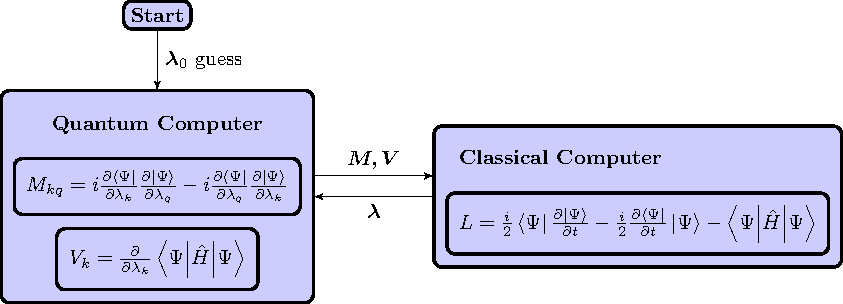
\includegraphics[width=\linewidth]{img/variation_figure.pdf}
  \caption{Visualization of the variational algorithm}
  \label{fig:TDVP}
\end{figure}
%
To solve these differential equations we use the \gls{tdvp}, which is an iterative method in which we start with a best guess $\bm \lambda(0)$, calculate the matrices $\bm M$ and $\bm V$ based on $\bm \lambda(0)$.
Then, we use these matrices to evolve $\bm \lambda(0)$ for a small amount of time into $\bm \lambda(\delta_t)$.
The process is repeated until the goal time $n\cdot\delta_t = T$ is reached.
We propose the use of a quantum circuit similar to Li's \cite{benjamin} and Ekert's \shortcite{ekert} to calculate the elements of the matrices $\bm M$ and $\bm V$ for each system of differential equations in each step of the iteration.
Figure \ref{fig:TDVP} illustrates this process, while figure \ref{fig:flowchart1} shows a broad view of the algorithm.

\begin{figure}[hb!]
	\centering
  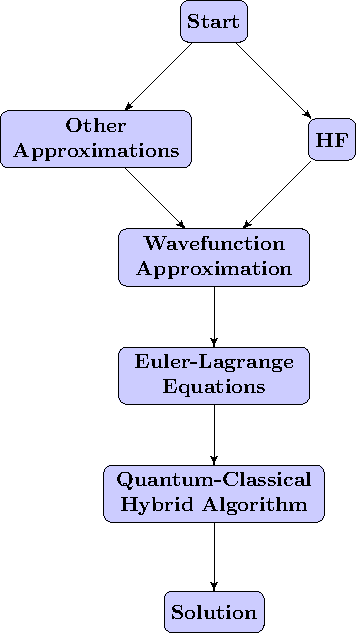
\includegraphics[width=.7\linewidth]{flowcharts/flowchart1.pdf}
  \caption{Abbreviated flowchart of the process to obtain a more accurate wavefunction for our electrons}
  \label{fig:flowchart1}
\end{figure}

\section{\textbf{Time Dependant Variational Principle (TDVP)}}\label{sec:tdvp}
%\shortcite{broeckhove} \cite{kramer}
First, we must obtain an approximation of the wavefunction for our simulation. That is done by applying a unitary transformation $\hat U$ to a initial state $\ket 0$.
We find the \gls {hf} approximation by following through Fukutome's method\cite{fukutome}. After doing so, we need to derive the dynamics of our system.

\subsection{\textbf{Wavefunction approximation}}

Here, we will obtain an expression for our trial wavefunction using Fukutome’s unitary representation \shortcite{fukutome}: 
$\ket \Psi = \hat U (\bm u_\lambda) \ket 0$,
where henceforth $\ket \Psi$ and $\ket 0$ denote the general and reference \gls{hf} states, respectively, cf. Eq. \ref{eq:slaterdet}.
In general, the matrix $\bm u_\lambda$ has an intricate structure, cf. Eq. \ref{eq:ulambda}.
Therefore, in this first attempt, we will adopt a chemical model system that leads to a simpler form of $\bm u_\lambda$.
Specifically, we will assume a system made up of several units (atoms or molecules) each of them having 2 electrons with spin up and down, respectively.
In addition, each electron has available one occupied spin-orbital $\phi_{\oo 0}$ and one unoccupied spin-orbital $\phi_{\uo 0}$.
Thus, the total number of spin-orbitals $\orb = 2\elec$, where $\elec$ is the total number of electrons.
In this scheme, each electron state can be assigned to a single qubit with a computational basis
$\ket 0 = \phi_{\oo 0}$ and $\ket 1 = \phi_{\uo 0}$.
Examples of this model system range from a single $\text{H}_2$ molecule to a crystal made up of well-separated $\text{H}_2$ molecules (well-separated to justify the approximation of two spin-orbitals per electron). 
Within this model system, $\bm u_\lambda$ decomposes as:
%Here we obtain an expression for our wavefunction using the \gls{hf} method: $\ket\Psi = \bm u_\lambda \ket 0$.
%One approximation we can introduce here is that $\uparrow$ spin orbitals only mix with $\uparrow$ spin orbitals, and
%$\downarrow$ spin orbitals only mix with $\downarrow$ spin orbitals.
%Applying this to decompose $\bm u_\lambda$:
\begin{equation}
	\begin{split}
	\label {eq:udecomposition}
	\bm u_\lambda
	= \bigotimes_{\uo 0 \oo 0}^N u_{\lambda_{\uo 0 \oo 0}}
	\end{split}
\end{equation}
%
where $\otimes$ is the Kronecker product and the $2\times2$ unitary matrix $\bm u_{\lambda_{\uo 0 \oo 0}}$ per electron is:
%Assuming $\elec = 2$ and $\orb = 4$ for a 2-electron system where each electron has 2 orbitals,  we find, from \shortcite{fukutome}:
%
\begin{align*}
	\bm u_{\lambda_{\uo 0 \oo 0}} 
	&= \begin{bmatrix}\bm C(\lambda_{\uo 0 \oo 0}) & \bm -\bm S^\dagger(\lambda_{\uo 0 \oo 0}) \\ \bm S(\lambda_{\uo 0 \oo 0}) & \tilde {\bm C}(\lambda_{\uo 0 \oo 0})\end{bmatrix} \in \mathbb{\bm C}^{2\times 2}
\end{align*}
%
Since 
$\bm u_{\lambda_\ind 0} \in \mathbb{C}^{2\times2}$, it is a single-qubit operator. This means each of its elements
$\bm C(\lambda)$, $\bm S(\lambda)$, $\tilde {\bm C}(\lambda) \in \mathbb{C}$ , and $\lambda_\ind 0 \in \mathbb{C}$. After some calculation, their values are:
%
\begin{align*}
	S(\lambda_\ind 0) 
	&= \sum_{k=0}^\infty \frac{(-1)^k}{(2k + 1)!}\lambda_\ind 0({\lambda_\ind 0}^\dagger{\lambda_\ind 0})^k \\
	&= \sum_{k=0}^\infty \frac{(-1)^k}{(2k + 1)!}\lambda_\ind 0({\lambda_\ind 0}^*\lambda_\ind 0)^k \\
	&= \sum_{k=0}^\infty \frac{(-1)^k}{(2k + 1)!}\lambda_\ind 0\frac{\abs{\lambda_\ind 0}}{\abs{\lambda_\ind 0}}(\abs{\lambda_\ind 0}^2)^k \\
	&= \sum_{k=0}^\infty \frac{(-1)^k}{(2k + 1)!}\frac{\lambda_\ind 0}{\paren{\lambda_\ind 0{\lambda_\ind 0}^*}^\frac 1 2}\abs{\lambda_\ind 0}^{2k + 1} \\
	&= \sum_{k=0}^\infty \frac{(-1)^k}{(2k + 1)!}\paren{\frac{\lambda_\ind 0}{\lambda_\ind 0^*}}^\frac 1 2\abs{\lambda_\ind 0}^{2k + 1} \\
	&= \paren{\frac{\lambda_\ind 0}{\lambda_\ind 0^*}}^\frac 1 2\sum_{k=0}^\infty \frac{(-1)^k}{(2k + 1)!}\abs{\lambda_\ind 0}^{2k + 1} \\
	&= \paren{\frac{\lambda_\ind 0}{\lambda_\ind 0^*}}^\frac 1 2\s{\abs{\lambda_\ind 0}} 
\end{align*}
\begin{align*}
	S^\dagger({\lambda_\ind 0}) 
	&= \paren{\paren{\frac{\lambda_\ind 0}{\lambda_\ind 0^*}}^\frac 1 2\s{\abs{\lambda_\ind 0}}}^\dagger \\
	&= \paren{\paren{\frac{\lambda_\ind 0}{\lambda_\ind 0^*}}^\frac 1 2\s{\abs{\lambda_\ind 0}}}^* \\
	&= \paren{\frac{\lambda_\ind 0^*}{\lambda_\ind 0}}^\frac 1 2\s{\abs{\lambda_\ind 0}} 
\end{align*}
\begin{align*}
	C(\lambda_\ind 0) 
	&= I_1 + \sum_{k=1}^\infty \frac{(-1)^k}{(2k)!}(\lambda_\ind 0^\dagger{\lambda_\ind 0})^k \\
	&= 1 + \sum_{k=1}^\infty \frac{(-1)^k}{(2k)!}(\lambda_\ind 0^*{\lambda_\ind 0})^k \\
	&= \sum_{k=0}^\infty \frac{(-1)^k}{(2k)!}(\abs{\lambda_\ind 0}^2)^k \\
	&= \sum_{k=0}^\infty \frac{(-1)^k}{(2k)!}\abs{\lambda_\ind 0}^{2k} \\
	&= \co {\abs{\lambda_\ind 0}} 
\end{align*}
\begin{align*}
	\tilde C({\lambda_\ind 0}) 
	&= I_{(2-1)} + \sum_{k=1}^\infty \frac{(-1)^k}{(2k)!}(\lambda_\ind 0{\lambda_\ind 0}^\dagger)^k \\
	&= 1 + \sum_{k=1}^\infty \frac{(-1)^k}{(2k)!}(\lambda_\ind 0{\lambda_\ind 0}^*)^k \\
	&= \sum_{k=0}^\infty \frac{(-1)^k}{(2k)!}\abs{\lambda_\ind 0}^{2k} \\
	&= \co {\abs{\lambda_\ind 0}} 
\end{align*}
%
Theorem 4.1 from \cite{nielsen} states that a single-qubit unitary gate $U$ can be written as $U = \exp(i\alpha) \bm R_z(\beta)\bm R_y(\gamma)\bm R_z(\delta)$ in terms of 4 real variables (parameters) $\alpha, \beta, \gamma, \delta$.
We can now apply the theorem to decompose this unitary matrix into an exponential term and three rotations:
%
\begin{align*}
	\bm u_{\lambda_\ind 0}
	&= \begin{bmatrix}
		C(\lambda_\ind 0) & \textbf -S^\dagger({\lambda_\ind 0}) \\ 
		S(\lambda_\ind 0) & \tilde C({\lambda_\ind 0})
	\end{bmatrix} \\
	&= \begin{bmatrix}
		\co{\abs{\lambda_\ind 0}} & -\left(\frac{\lambda_\ind 0^*}{\lambda_\ind 0}\right)^{\frac 1 2}\s{\abs{\lambda_\ind 0}} \\
		\left(\frac{\lambda_\ind 0}{\lambda_\ind 0^*}\right)^{\frac 1 2}\s{\abs{\lambda_\ind 0}} &  \co{\abs{\lambda_\ind 0}}
	\end{bmatrix}\\
	&= \begin{bmatrix}
		\co{\rho_\ind 0} & -e^{-i\omega_\ind 0}\s{\rho_\ind 0} \\
		e^{i\omega_\ind 0}\s{\rho_\ind 0} &  \co{\rho_\ind 0}
	\end{bmatrix}\\
	&= \begin{bmatrix}
		e^{i\left(\alpha - \frac \beta 2 + \frac \delta 2 \right)}\co{\frac \gamma 2} & -e^{i\left(\alpha - \frac \beta 2 + \frac \delta 2 \right)}\s{\frac \gamma 2} \\
		e^{i\left(\alpha - \frac \beta 2 + \frac \delta 2 \right)}\s{\frac \gamma 2} &  e^{i\left(\alpha - \frac \beta 2 + \frac \delta 2 \right)}\co{\frac \gamma 2}
	\end{bmatrix}\\
	&= e^{i\alpha}\bm R_z(\beta)\bm R_y(\gamma)\bm R_z(\delta) 
\end{align*}
%
Solving for $\alpha, \beta, \gamma, \delta$ in terms of $\rho_\ind 0 = \abs{\lambda_\ind 0}, \omega_\ind 0 = \arg \lambda_\ind 0$, we get 
%
${\alpha = 0}$; 
${\beta = \omega_\ind 0}$; 
${\gamma = 2\rho_\ind 0}$;
${\delta = -\omega_\ind 0}$. Finally:
%
\begin{equation}
	\begin{split}
	\label{eq:urotation}
	\bm u_{\lambda_\ind 0}
	&= \bm R_z(\omega_\ind 0)\bm R_y(2\rho_\ind 0)\bm R_z(-\omega_\ind 0) \\
	&= \begin{bmatrix}
		e^{-i\frac {\omega_\ind 0} 2} & 0 \\
		0 &  e^{i\frac {\omega_\ind 0} 2}
	\end{bmatrix}
	\begin{bmatrix}
		\co{\rho_\ind 0} & -\s{\rho_\ind 0} \\
		\s{\rho_\ind 0} &  \co{\rho_\ind 0}
	\end{bmatrix}
	\begin{bmatrix}
		e^{i\frac {\omega_\ind 0} 2} & 0 \\
		0 &  e^{-i\frac {\omega_\ind 0} 2}
	\end{bmatrix} 
	\end{split}
\end{equation}
%
Notice now that $\det \paren{\bm u_{\lambda_\ind 0}} = 1$, and $\bm u_{\lambda_\ind 0}$ belongs to the special unitary group $SU(2)$, $\bm u_{\lambda_\ind 0} \in SU(2)$.
%
We shall now rewrite $\bm u_{\lambda_\ind 0}$ in terms of the identity and Pauli matrices ($\bm I, \bm X, \bm Y, \bm Z$):
\begin{align*}
	\bm u_{\lambda_\ind 0}
	&= \bm R_z(\omega_\ind 0)\bm R_y(2\rho_\ind 0)\bm R_z(-\omega_\ind 0) \\
	& = \paren{\co{\frac {\omega_\ind 0} 2}I - i\s{\frac {\omega_\ind 0} 2}Z}
	\cdot \paren{\co{\rho_\ind 0}I - i\s{\rho_\ind 0}Y}\\
	& \quad \cdot
	\paren{\co{\frac {\omega_\ind 0} 2}I + i\s{\frac {\omega_\ind 0} 2}Z} \\
	& = 
	\left(
		\co{\frac {\omega_\ind 0} 2} \co {\rho_\ind 0} I 
		- i\co{\frac {\omega_\ind 0} 2} \s {\rho_\ind 0} Y 
		- i\s{\frac {\omega_\ind 0} 2} \co {\rho_\ind 0} Z
	\right. \\
	&\quad \left.
		- \s{\frac {\omega_\ind 0} 2} \s {\rho_\ind 0} ZY
	\right)
	\cdot \paren{\co{\frac {\omega_\ind 0} 2}I + i\s{\frac {\omega_\ind 0} 2}Z} \\
	\intertext{Substituting $ZY = -iX$:}
	& = 
	\left(
		\co{\frac {\omega_\ind 0} 2} \co {\rho_\ind 0} I 
		- i\co{\frac {\omega_\ind 0} 2} \s {\rho_\ind 0} Y 
		- i\s{\frac {\omega_\ind 0} 2} \co {\rho_\ind 0} Z
	\right. \\
	&\quad \left.
		+ i\s{\frac {\omega_\ind 0} 2} \s {\rho_\ind 0} X
	\right)
	\paren{\co{\frac {\omega_\ind 0} 2}I + i\s{\frac {\omega_\ind 0} 2}Z} \\
	& = 
		\cosq{\frac {\omega_\ind 0} 2} \co {\rho_\ind 0} I 
		- i\cosq{\frac {\omega_\ind 0} 2} \s {\rho_\ind 0} Y 
	\\
	& \quad 
		- i\s{\frac {\omega_\ind 0} 2} \co{\frac {\omega_\ind 0} 2} \co {\rho_\ind 0} Z 
		+ i\s{\frac {\omega_\ind 0} 2} \co{\frac {\omega_\ind 0} 2} \s {\rho_\ind 0} X 
	\\
	& \quad 
		+ i \s{\frac {\omega_\ind 0} 2} \co{\frac {\omega_\ind 0} 2} \co {\rho_\ind 0} Z
		+ \s{\frac {\omega_\ind 0} 2} \co{\frac {\omega_\ind 0} 2} \s {\rho_\ind 0} YZ
	\\
	& \quad 
		+ \ssq{\frac {\omega_\ind 0} 2} \co {\rho_\ind 0} I
		- \ssq{\frac {\omega_\ind 0} 2} \s {\rho_\ind 0} XZ
	\intertext{Grouping up similar terms and substituting $YZ = iX$:}
	& = 
		\co {\rho_\ind 0} \paren{
		\cosq{\frac {\omega_\ind 0} 2}  I 
		+ \ssq{\frac {\omega_\ind 0} 2} I
		}
	\\
	& \quad
		+ \co {\rho_\ind 0} \paren{
		- i\s{\frac {\omega_\ind 0} 2} \co{\frac {\omega_\ind 0} 2}  Z 
		+ i \s{\frac {\omega_\ind 0} 2} \co{\frac {\omega_\ind 0} 2}  Z
		}
	\\
	& \quad 
		+ \s {\rho_\ind 0} \paren{
		- \ssq{\frac {\omega_\ind 0} 2} XZ
		- i\cosq{\frac {\omega_\ind 0} 2} Y 
		}
	\\
	& \quad 
		+ \s {\rho_\ind 0} \paren{
		i\s{\frac {\omega_\ind 0} 2} \co{\frac {\omega_\ind 0} 2} X 
		+ i\s{\frac {\omega_\ind 0} 2} \co{\frac {\omega_\ind 0} 2} X
	}
	\\
	\intertext{Simplifying some expressions and substituting $XZ = -iY$:}
	& = 
		\co {\rho_\ind 0} I
		+ \co {\rho_\ind 0} \paren{0}
		- i \s {\rho_\ind 0} \paren{
		\cosq{\frac {\omega_\ind 0} 2} Y 
		-  \ssq{\frac {\omega_\ind 0} 2} Y
		}
	\\
	& \quad 
		+ i \s \rho_\ind 0
		2\s{\frac {\omega_\ind 0} 2} \co{\frac {\omega_\ind 0} 2} X 
	\\
	& = 
		\co {\rho_\ind 0} I
		- i \s {\rho_\ind 0} \co{\omega_\ind 0} Y 
		+ i \s {\rho_\ind 0} \s{\omega_\ind 0} X
\end{align*}
%
%Now, applying $\bm u_\lambda$ to a vacuum, we get:
At this point, we will concentrate on a system with $\elec = 2 \implies \orb = 4$, e.g., the $\text{H}_2$ molecule. If we apply $\bm u_\lambda$ to the ground state of the model system as the reference \gls{hf} state $\ket 0$, we get:
%
\begin{equation}
	\begin{split}
		\label{eq:psirw}
	\ket \Psi 
	&= \bm u_{\lambda_\ind 0} \otimes \bm u_{\lambda_\ind 1} \ket 0 \\
	&= \bm u_{\lambda_\ind 0} \otimes \bm u_{\lambda_\ind 1} \ket {\psi_{\oo 0} \psi_{\oo 1} } \\
	&= \bm u_{\lambda_\ind 0} \ket {\psi_{\oo 0}} \otimes \bm u_{\lambda_\ind 1} \ket{\psi_{\oo 1} } \\
	&= \ket {\co {\rho_\ind 0} \psi_{\oo 0} + e^{i\omega_\ind 0}\s {\rho_\ind 0} \psi_{\uo 0}} \otimes
	\ket {\co {\rho_\ind 1} \psi_{\oo 1} + e^{i\omega_\ind 1}\s {\rho_\ind 1} \psi_{\uo 1}} \\
	&= \co {\rho_\ind 0 }\co {\rho_\ind 1}\ket {\psi_{\oo 0}\psi_{\oo 1}}
	+ e^{i\omega_\ind 1}\co {\rho_\ind 0 }\s {\rho_\ind 1}\ket {\psi_{\oo 0}\psi_{\uo 1}} \\
	&\quad + e^{i\omega_\ind 0 }\s {\rho_\ind 0 }\co {\rho_\ind 1}\ket{\psi_{\uo 0} \psi_{\oo 1}} 
	+ e^{i\omega_\ind 0 }e^{i\omega_\ind 1}\s {\rho_\ind 0 }\s {\rho_\ind 1}\ket{\psi_{\uo 0} \psi_{\uo 1}} 
	\end{split}
\end{equation}
%
Note here that our wavefunction $\ket \Psi$ is a function of four real variables $\omega_\ind 0, \omega_\ind 1, \rho_\ind 0, \rho_\ind 1$. It can also be written as a tensor product of two single-qubit operators, where $\bm u_{\lambda_{\ind 0}}$ acts on $\uparrow$ spin orbitals and $\bm u_{\lambda_{\ind 1}}$ acts on $\downarrow$ spin orbitals.

%-------------------------------------------------------------------------------------

\section {\textbf{Circuit for 2-electron model}}

We propose to use a quantum circuit to evaluate the matrices $\bm M$ and $\bm V$. To do so, we must adapt Li's \shortcite{benjamin} algorithm, which is a variation of Ekert's \shortcite{ekert} quantum circuit, to work with our reduced number of variables.
%
\subsection {\textbf{Dynamics}}

The next step to use the \gls{tdvp} would be to evaluate $\bm M$ and $\bm V$.
%To do so, we need to set up the Lagrangian and solve the Euler-Lagrange equation system.
To do so, we construct the quantum Lagrangian for our trial wave function as explained in the introduction of this chapter:
\[
	L = \frac{\sandwich{\Psi(t)}{\frac{i}{2}\left(\overrightarrow{\pd t} - \overleftarrow{\pd t}\right) - \hat H}{\Psi(t)}}{\braket{\Psi(t)}{\Psi(t)}}
\]
%
Our wavefunction $\Psi$ is generated by a unitary transformation and, therefore, is normalized to 1 at every time. This means $\braket{\Psi(t)}{\Psi(t)} = 1$. We now also rewrite the variables of $\ket{\Psi}$ as 
$\lambda_1 = \omega_\ind 1; \lambda_2 = \omega_\ind 0; \lambda_3 = \rho_\ind 1; \lambda_4 = \rho_\ind 0$.
The order of the numbering of the new lambda variables is important and shall be discussed later in Eq. \ref{eq:rdecomposition}. 
This means we can express the Lagrangian as:
\begin{equation}
	\begin{split}
		\label{eq:lagrangian}
		L &= \sandwich{\Psi}{\frac{i}{2}\left(\overrightarrow{\pd t} - \overleftarrow{\pd t}\right) - \hat H}{\Psi} \\
		  &= \frac{i}{2}\bra{\Psi}{\kpp t} - \frac{i}{2}{\bpp{t}}\ket{\Psi} - \sandwich{\Psi}{\hat H}{\Psi} \\
		  &= 	
			\sum_j \frac{i}{2}\bra{\Psi}{\kpp {\lambda_j}} \dot \lambda_j
		- 	\sum_j \frac{i}{2}{\bpp{\lambda_j}}\ket{\Psi}\dot{\lambda_j}
		- \sandwich{\Psi}{\hat H}{\Psi}
	\end{split}
\end{equation}
%
We now take the derivative of \ref{eq:lagrangian} with regards to $\lambda_k$ for $k \in \{1, 2, 3, 4\}$:
%
\begin{equation*}
	\begin{split}
	\pd{\lambda_k} L &= 	
	\phantom{-}\sum_j \frac{i}{2}\bra{\Psi}{\kppd {\lambda_k}{\lambda_j}} \dot \lambda_j
	+	\sum_j \frac{i}{2}\bpp{\lambda_k}{\kpp {\lambda_j}} \dot \lambda_j \\
	&\quad -\sum_j \frac{i}{2}{\bppd{\lambda_k}{\lambda_j}}\ket{\Psi}\dot{\lambda_j}
	- 	\sum_j \frac{i}{2}{\bpp{\lambda_j}}\kpp{\lambda_k}\dot{\lambda_j}\\
	&\quad -\pd{\lambda_k} \sandwich{\Psi}{\hat H}{\Psi}
	\end{split}
\end{equation*}
%
And take the derivative of \ref{eq:lagrangian} with regards to $\dot{\lambda_k} = \dd{t} \lambda_k$ for $k \in \{1, 2, 3, 4\}$:
%
\begin{equation*}
	\begin{split}
		\label{eq:euler-lagrange}
		\pd{\dot{\lambda_k}} L &=
		\frac{i}{2}\bra{\Psi}{\kpp {\lambda_k}}
	- 	\frac{i}{2}{\bpp{\lambda_k}}\ket{\Psi}
	\end{split}
\end{equation*}
%
Now, since the Euler-Lagrange equations for the variables are $\pd{\lambda_k} L = \ddt \pd{\dot {\lambda_k}} L$, we take the derivative of the expression above with regards to time:
%
\begin{equation*}
	\begin{split}
		\ddt \pd{\dot{\lambda_k}} L &=
		\sum_j \frac{i}{2}\bpp{\lambda_j}{\kpp {\lambda_k}} \dot \lambda_j
	+	\sum_j \frac{i}{2}\bra{\Psi}{\kppd {\lambda_j}{\lambda_k}} \dot \lambda_j \\
    	&- 	\sum_j \frac{i}{2}{\bppd{\lambda_j}{\lambda_k}}\ket{\Psi}\dot{\lambda_j}
	- 	\sum_j \frac{i}{2}{\bpp{\lambda_k}}\kpp{\lambda_j}\dot{\lambda_j}
	\end{split}
\end{equation*}
%
We can now obtain the Euler-Lagrange equations, and the only terms that do not cancel out are as follows:
%
\begin{equation*}
	\begin{split}
		\ddt \pd{\dot{\lambda_k}} L 
	&=	\pd{\lambda_k} L
	\\
	 	\sum_j i \bpp{\lambda_k} \kpp{\lambda_j}\dot{\lambda_j}
	-	\sum_j i \bpp{\lambda_j} \kpp{\lambda_k}\dot{\lambda_j}
	&= 	\pd{\lambda_k}\sandwich{\Psi}{\hat H}{\Psi}
	\end{split}
\end{equation*}
%
These equations can be put into matrix form:
%
\begin{equation}
	\begin{split}
		\label{eq:matrixderiv}
		&i \left [ \bpp{\lambda_k} \kpp{\lambda_q} 
			- \bpp{\lambda_q} \kpp{\lambda_k} \right ]_{kq}
		\cdot 	\left[ \dot \lambda_q \right]_q
		=	\left[\pd{\lambda_k}\sandwich{\Psi}{\hat H}{\Psi}\right]_k 
	\\% -----------------------Second Equation Line---------------------------------------
		\span i
		\begin{pmatrix}
			0 
			&  \bpp{\lambda_1} \kpp{\lambda_2} -  \bpp{\lambda_2} \kpp{\lambda_1} 
			&  \bpp{\lambda_1} \kpp{\lambda_3} -  \bpp{\lambda_3} \kpp{\lambda_1} 
			&  \bpp{\lambda_1} \kpp{\lambda_4} -  \bpp{\lambda_4} \kpp{\lambda_1} 
		\\% --------------------------Second Matrix Line------------------------------
			 \bpp{\lambda_2} \kpp{\lambda_1} -  \bpp{\lambda_1} \kpp{\lambda_2} 
			& 0
			& \bpp{\lambda_2} \kpp{\lambda_3} -  \bpp{\lambda_3} \kpp{\lambda_2} 
			& \bpp{\lambda_2} \kpp{\lambda_4} -  \bpp{\lambda_4} \kpp{\lambda_2} 
		\\% --------------------------Third  Matrix Line------------------------------
			 \bpp{\lambda_3} \kpp{\lambda_1} -  \bpp{\lambda_1} \kpp{\lambda_3} 
			& \bpp{\lambda_3} \kpp{\lambda_2} -  \bpp{\lambda_2} \kpp{\lambda_3} 
			& 0
			& \bpp{\lambda_3} \kpp{\lambda_4} -  \bpp{\lambda_4} \kpp{\lambda_3} 
		\\% --------------------------Fourth Matrix Line------------------------------
			 \bpp{\lambda_4} \kpp{\lambda_1} -  \bpp{\lambda_1} \kpp{\lambda_4} 
			& \bpp{\lambda_4} \kpp{\lambda_2} -  \bpp{\lambda_2} \kpp{\lambda_4} 
			& \bpp{\lambda_4} \kpp{\lambda_3} -  \bpp{\lambda_3} \kpp{\lambda_4} 
			& 0
		\end{pmatrix} 
	\\
		&\times
		\begin{pmatrix}
			\dot \lambda_1 \\
			\dot \lambda_2 \\
			\dot \lambda_3 \\
			\dot \lambda_4 
		\end{pmatrix} 
		=
		\begin{pmatrix}
			\pd {\lambda_1} \sandwich{\Psi}{\hat H}{\Psi}\\
			\pd {\lambda_2} \sandwich{\Psi}{\hat H}{\Psi}\\
			\pd {\lambda_3} \sandwich{\Psi}{\hat H}{\Psi}\\
			\pd {\lambda_4} \sandwich{\Psi}{\hat H}{\Psi}\\
		\end{pmatrix} 
	\\
		&\sum_q M_{kq} \dot \lambda_q = V_k
	\end{split}
\end{equation}
%
Where:
%
\begin{equation*}
	\begin{split}
	M_{kq} 
	&= 
	 	i \bpp{\lambda_k} \kpp{\lambda_q} - i \bpp{\lambda_q} \kpp{\lambda_k} 
	\\
	V_k 
	&= 	\pd{\lambda_k}\sandwich{\Psi}{\hat H}{\Psi} \\
	\end{split}
\end{equation*}
%
We can now turn back to the previous expression of $\ket{\Psi}$ in terms of the variational parameters to calculate the elements of $\bm M$. First we calculate the values of the derivatives of $\ket \Psi$ with respect to $\rho_\ind 0 ,\omega_\ind 0$ and $\rho_\ind 1 , \omega_\ind 1$.
%
\begin{align*}
	\ket \Psi 
	&= \co {\rho_\ind 0}\co {\rho_\ind 1}\ket {\psi_{\oo 0}\psi_{\oo 1}}
	+ e^{i\omega_\ind 1}\co {\rho_\ind 0 }\s {\rho_\ind 1}\ket {\psi_{\oo 0}\psi_{\uo 1}} \\
	&\quad + e^{i\omega_\ind 0}\s {\rho_\ind 0}\co {\rho_\ind 1}\ket{\psi_{\uo 0} \psi_{\oo 1}} 
	+ e^{i\omega_\ind 0}e^{i\omega_\ind 1}\s {\rho_\ind 0}\s {\rho_\ind 1}\ket{\psi_{\uo 0} \psi_{\uo 1}} 
	\\
	\pd {\rho_\ind 0 } \ket \Psi 
	&= -\s {\rho_\ind 0}\co {\rho_\ind 1}\ket {\psi_{\oo 0}\psi_{\oo 1}}
	- e^{i\omega_\ind 1}\s {\rho_\ind 0 }\s {\rho_\ind 1}\ket {\psi_{\oo 0}\psi_{\uo 1}} \\
	&\quad + e^{i\omega_\ind 0}\co {\rho_\ind 0}\co {\rho_\ind 1}\ket{\psi_{\uo 0} \psi_{\oo 1}} 
	+ e^{i\omega_\ind 0}e^{i\omega_\ind 1}\co {\rho_\ind 0}\s {\rho_\ind 1}\ket{\psi_{\uo 0} \psi_{\uo 1}} 
	\\
	\pd {\omega_\ind 0} \ket \Psi 
	&= \co {\rho_\ind 0}\co {\rho_\ind 1}\ket {\psi_{\oo 0}\psi_{\oo 1}}
	+ e^{i\omega_\ind 1}\co {\rho_\ind 0 }\s {\rho_\ind 1}\ket {\psi_{\oo 0}\psi_{\uo 1}} \\
	&\quad + ie^{i\omega_\ind 0}\s {\rho_\ind 0}\co {\rho_\ind 1}\ket{\psi_{\uo 0} \psi_{\oo 1}} 
	+ ie^{i\omega_\ind 0}e^{i\omega_\ind 1}\s {\rho_\ind 0}\s {\rho_\ind 1}\ket{\psi_{\uo 0} \psi_{\uo 1}} 
	\\
	\pd {\rho_\ind 1 } \ket \Psi 
	&= -\co {\rho_\ind 0}\s {\rho_\ind 1}\ket {\psi_{\oo 0}\psi_{\oo 1}}
	+ e^{i\omega_\ind 1}\co {\rho_\ind 0 }\co {\rho_\ind 1}\ket {\psi_{\oo 0}\psi_{\uo 1}} \\
	&\quad - e^{i\omega_\ind 0}\s {\rho_\ind 0}\s {\rho_\ind 1}\ket{\psi_{\uo 0} \psi_{\oo 1}} 
	+ e^{i\omega_\ind 0}e^{i\omega_\ind 1}\s {\rho_\ind 0}\co {\rho_\ind 1}\ket{\psi_{\uo 0} \psi_{\uo 1}} 
	\\
	\pd {\omega_\ind 1} \ket \Psi 
	&= \co {\rho_\ind 0}\co {\rho_\ind 1}\ket {\psi_{\oo 0}\psi_{\oo 1}}
	+ ie^{i\omega_\ind 1}\co {\rho_\ind 0 }\s {\rho_\ind 1}\ket {\psi_{\oo 0}\psi_{\uo 1}} \\
	&\quad + e^{i\omega_\ind 0}\s {\rho_\ind 0}\co {\rho_\ind 1}\ket{\psi_{\uo 0} \psi_{\oo 1}} 
	+ ie^{i\omega_\ind 0}e^{i\omega_\ind 1}\s {\rho_\ind 0}\s {\rho_\ind 1}\ket{\psi_{\uo 0} \psi_{\uo 1}} 
\end{align*}
%
Now we need have the partial derivatives of $\ket\Psi$, but we need to find the expressions for their duals (i.e., their adjoint expressions). We can take the dual of $\ket \Psi$ from \ref{eq:psirw}:
%
\begin{equation}
	\label{eq:dualpsirw}
	\begin{split}
		\bra \Psi &= \ket\Psi^\dagger
	= \left(\co {\rho_\ind 0 }\co {\rho_\ind 1}\ket {\psi_{\oo 0}\psi_{\oo 1}}
	+ e^{i\omega_\ind 1}\co {\rho_\ind 0 }\s {\rho_\ind 1}\ket {\psi_{\oo 0}\psi_{\uo 1}} \right .\\
	& \left . \quad + e^{i\omega_\ind 0 }\s {\rho_\ind 0 }\co {\rho_\ind 1}\ket{\psi_{\uo 0} \psi_{\oo 1}} 
	+ e^{i\omega_\ind 0 }e^{i\omega_\ind 1}\s {\rho_\ind 0 }\s {\rho_\ind 1}\ket{\psi_{\uo 0} \psi_{\uo 1}} \right)^\dagger \\
	&= \co {\rho_\ind 0}\co {\rho_\ind 1}\bra {\psi_{\oo 0}\psi_{\oo 1}}
	+ e^{ -i \omega_\ind 1}\co {\rho_\ind 0 }\s {\rho_\ind 1}\bra {\psi_{\oo 0}\psi_{\uo 1}} \\
	&\quad + e^{ -i \omega_\ind 0}\s {\rho_\ind 0}\co {\rho_\ind 1}\bra{\psi_{\uo 0} \psi_{\oo 1}} 
	+ e^{ -i \omega_\ind 0}e^{ -i \omega_\ind 1}\s {\rho_\ind 0}\s {\rho_\ind 1}\bra{\psi_{\uo 0} \psi_{\uo 1}} 
	\end{split}
\end{equation}
%
And take the derivatives of \ref{eq:dualpsirw}:
%
\begin{align*}
	\pd {\rho_\ind 0 } \bra \Psi 
	&= -\s {\rho_\ind 0}\co {\rho_\ind 1}\bra {\psi_{\oo 0}\psi_{\oo 1}}
	- e^{ -i \omega_\ind 1}\s {\rho_\ind 0 }\s {\rho_\ind 1}\bra {\psi_{\oo 0}\psi_{\uo 1}} \\
	&\quad + e^{ -i \omega_\ind 0}\co {\rho_\ind 0}\co {\rho_\ind 1}\bra{\psi_{\uo 0} \psi_{\oo 1}} 
	+ e^{ -i \omega_\ind 0}e^{ -i \omega_\ind 1}\co {\rho_\ind 0}\s {\rho_\ind 1}\bra{\psi_{\uo 0} \psi_{\uo 1}} 
	\\
	\pd {\omega_\ind 0} \bra \Psi 
	&=
	-i e^{ -i \omega_\ind 0}\s {\rho_\ind 0}\co {\rho_\ind 1}\bra{\psi_{\uo 0} \psi_{\oo 1}} 
	-i e^{ -i \omega_\ind 0}e^{ -i \omega_\ind 1}\s {\rho_\ind 0}\s {\rho_\ind 1}\bra{\psi_{\uo 0} \psi_{\uo 1}} 
	\\
	\pd {\rho_\ind 1 } \bra \Psi 
	&= -\co {\rho_\ind 0}\s {\rho_\ind 1}\bra {\psi_{\oo 0}\psi_{\oo 1}}
	+ e^{ -i \omega_\ind 1}\co {\rho_\ind 0 }\co {\rho_\ind 1}\bra {\psi_{\oo 0}\psi_{\uo 1}} \\
	&\quad - e^{ -i \omega_\ind 0}\s {\rho_\ind 0}\s {\rho_\ind 1}\bra{\psi_{\uo 0} \psi_{\oo 1}} 
	+ e^{ -i \omega_\ind 0}e^{ -i \omega_\ind 1}\s {\rho_\ind 0}\co {\rho_\ind 1}\bra{\psi_{\uo 0} \psi_{\uo 1}} 
	\\
	\pd {\omega_\ind 1} \bra \Psi 
	&= 
	-i e^{ -i \omega_\ind 1}\co {\rho_\ind 0 }\s {\rho_\ind 1}\bra {\psi_{\oo 0}\psi_{\uo 1}}
	-i e^{ -i \omega_\ind 0}e^{ -i \omega_\ind 1}\s {\rho_\ind 0}\s {\rho_\ind 1}\bra{\psi_{\uo 0} \psi_{\uo 1}} 
\end{align*}
%
Finally, we have all the information needed to calculate the elements of the $\bm M$ matrix in \ref{eq:matrixderiv}. First, we notice that the metric matrix is in this case with real variational parameters skew-symmetric (i.e., real anti-Hermitian: $\bm M = - \bm M^T$), since:
%
\begin{align*}
	M_{kq} = 
	\bpp{\lambda_k} \kpp{\lambda_q}
	- \bpp{\lambda_q} \kpp{\lambda_k} = 
	- \paren
	{
		\bpp{\lambda_q} \kpp{\lambda_k}
		- \bpp{\lambda_k} \kpp{\lambda_q}
	}
	=M_{qk}
\end{align*}
%
We now calculate each element of the matrix $\bm M$:
%
\begin{enumerate}
	% item I
	\item $ \bpp{\rho_\ind 0} \kpp{\omega_\ind 0}
	- \bpp{\omega_\ind 0} \kpp{\rho_\ind 0}$

\begin{align*}
	&\left (
	-\s {\rho_\ind 0}\co {\rho_\ind 1}\bra {\psi_{\oo 0}\psi_{\oo 1}}
	- e^{ -i \omega_\ind 1}\s {\rho_\ind 0 }\s {\rho_\ind 1}\bra {\psi_{\oo 0}\psi_{\uo 1}}
	\right .
	\\
	&\left .
	\quad + e^{ -i \omega_\ind 0}\co {\rho_\ind 0}\co {\rho_\ind 1}\bra{\psi_{\uo 0} \psi_{\oo 1}} 
	+ e^{ -i \omega_\ind 0}e^{ -i \omega_\ind 1}\co {\rho_\ind 0}\s {\rho_\ind 1}\bra{\psi_{\uo 0} \psi_{\uo 1}} 
	\right )
	\\
	&\times \left (
	ie^{i\omega_\ind 0}\s {\rho_\ind 0}\co {\rho_\ind 1}\ket{\psi_{\uo 0} \psi_{\oo 1}} 
	+ ie^{i\omega_\ind 0}e^{i\omega_\ind 1}\s {\rho_\ind 0}\s {\rho_\ind 1}\ket{\psi_{\uo 0} \psi_{\uo 1}} 
	\right )
	\\
	&- \left (
	-i e^{ -i \omega_\ind 0}\s {\rho_\ind 0}\co {\rho_\ind 1}\bra{\psi_{\uo 0} \psi_{\oo 1}} 
	-i e^{ -i \omega_\ind 0}e^{ -i \omega_\ind 1}\s {\rho_\ind 0}\s {\rho_\ind 1}\bra{\psi_{\uo 0} \psi_{\uo 1}} 
	\right )
	\\
	&\times\left (
	-\s {\rho_\ind 0}\co {\rho_\ind 1}\ket {\psi_{\oo 0}\psi_{\oo 1}}
	- e^{i\omega_\ind 1}\s {\rho_\ind 0 }\s {\rho_\ind 1}\ket {\psi_{\oo 0}\psi_{\uo 1}}
	\right .
	\\
	&\left .
	\quad + e^{i\omega_\ind 0}\co {\rho_\ind 0}\co {\rho_\ind 1}\ket{\psi_{\uo 0} \psi_{\oo 1}} 
	+ e^{i\omega_\ind 0}e^{i\omega_\ind 1}\co {\rho_\ind 0}\s {\rho_\ind 1}\ket{\psi_{\uo 0} \psi_{\uo 1}} 
	\right )
	\intertext{Since we have an orthogonal basis, only matching brackets are nonzero:}
	% --------------------------------------Second System-----------------------------------
	&=
		i\s{\rho_\ind 0} \co{\rho_\ind 0}\cosq {\rho_\ind 1}
		+ i\s{\rho_\ind 0} \co{\rho_\ind 0}\ssq {\rho_\ind 1}
	\\
	&+
	i \s {\rho_\ind 0}\co {\rho_\ind 0}\cosq {\rho_\ind 1}
	+i \s {\rho_\ind 0}\co {\rho_\ind 0}\ssq {\rho_\ind 1}
	\\
	&=
	i\s{2\rho_\ind 0}
\end{align*}

	% item II
	\item $ \bpp{\rho_\ind 0} \kpp{\rho_\ind 1}
	- \bpp{\rho_\ind 1} \kpp{\rho_\ind 0}$


\begin{align*}
	&\left (
	-\s {\rho_\ind 0}\co {\rho_\ind 1}\bra {\psi_{\oo 0}\psi_{\oo 1}}
	- e^{ -i \omega_\ind 1}\s {\rho_\ind 0 }\s {\rho_\ind 1}\bra {\psi_{\oo 0}\psi_{\uo 1}} 
	\right .
	\\
	&\left .
	\quad + e^{ -i \omega_\ind 0}\co {\rho_\ind 0}\co {\rho_\ind 1}\bra{\psi_{\uo 0} \psi_{\oo 1}} 
	+ e^{ -i \omega_\ind 0}e^{ -i \omega_\ind 1}\co {\rho_\ind 0}\s {\rho_\ind 1}\bra{\psi_{\uo 0} \psi_{\uo 1}} 
	\right )
	\\
	&\times\left (
	-\co {\rho_\ind 0}\s {\rho_\ind 1}\ket {\psi_{\oo 0}\psi_{\oo 1}}
	+ e^{i\omega_\ind 1}\co {\rho_\ind 0 }\co {\rho_\ind 1}\ket {\psi_{\oo 0}\psi_{\uo 1}} 
	\right .
	\\
	&\left .
	\quad - e^{i\omega_\ind 0}\s {\rho_\ind 0}\s {\rho_\ind 1}\ket{\psi_{\uo 0} \psi_{\oo 1}} 
	+ e^{i\omega_\ind 0}e^{i\omega_\ind 1}\s {\rho_\ind 0}\co {\rho_\ind 1}\ket{\psi_{\uo 0} \psi_{\uo 1}} 
	\right )
	\\
	&- \left (
	-\co {\rho_\ind 0}\s {\rho_\ind 1}\bra {\psi_{\oo 0}\psi_{\oo 1}}
	+ e^{ -i \omega_\ind 1}\co {\rho_\ind 0 }\co {\rho_\ind 1}\bra {\psi_{\oo 0}\psi_{\uo 1}} 
	\right .
	\\
	&\left .
	\quad - e^{ -i \omega_\ind 0}\s {\rho_\ind 0}\s {\rho_\ind 1}\bra{\psi_{\uo 0} \psi_{\oo 1}} 
	+ e^{ -i \omega_\ind 0}e^{ -i \omega_\ind 1}\s {\rho_\ind 0}\co {\rho_\ind 1}\bra{\psi_{\uo 0} \psi_{\uo 1}} 
	\right )
	\\
	&\times \left (
	-\s {\rho_\ind 0}\co {\rho_\ind 1}\ket {\psi_{\oo 0}\psi_{\oo 1}}
	- e^{i\omega_\ind 1}\s {\rho_\ind 0 }\s {\rho_\ind 1}\ket {\psi_{\oo 0}\psi_{\uo 1}} 
	\right .
	\\
	&\left .
	\quad + e^{i\omega_\ind 0}\co {\rho_\ind 0}\co {\rho_\ind 1}\ket{\psi_{\uo 0} \psi_{\oo 1}} 
	+ e^{i\omega_\ind 0}e^{i\omega_\ind 1}\co {\rho_\ind 0}\s {\rho_\ind 1}\ket{\psi_{\uo 0} \psi_{\uo 1}} 
	\right )
	\\
	%Second Term---------------------------------------------------------------------
	&= \s {\rho_\ind 0}\co {\rho_\ind 0}\s {\rho_\ind 1}\co {\rho_\ind 1}
	- \s {\rho_\ind 0}\co {\rho_\ind 0}\s {\rho_\ind 1}\co {\rho_\ind 1}
	\\
	&- \s {\rho_\ind 0}\co {\rho_\ind 0}\s {\rho_\ind 1}\co {\rho_\ind 1}
	+ \s {\rho_\ind 0}\co {\rho_\ind 0}\s {\rho_\ind 1}\co {\rho_\ind 1}
	\\
	&- \s {\rho_\ind 0}\co {\rho_\ind 0}\s {\rho_\ind 1}\co {\rho_\ind 1}
	+ \s {\rho_\ind 0}\co {\rho_\ind 0}\s {\rho_\ind 1}\co {\rho_\ind 1}
	\\
	&+ \s {\rho_\ind 0}\co {\rho_\ind 0}\s {\rho_\ind 1}\co {\rho_\ind 1}
	- \s {\rho_\ind 0}\co {\rho_\ind 0}\s {\rho_\ind 1}\co {\rho_\ind 1}
	\\
	&= 0
\end{align*}

	% item III
	\item $ \bpp{\rho_\ind 0} \kpp{\omega_\ind 1}
	- \bpp{\omega_\ind 1} \kpp{\rho_\ind 0}$

\begin{align*}
	&\left (
	-\s {\rho_\ind 0}\co {\rho_\ind 1}\bra {\psi_{\oo 0}\psi_{\oo 1}}
	- e^{ -i \omega_\ind 1}\s {\rho_\ind 0 }\s {\rho_\ind 1}\bra {\psi_{\oo 0}\psi_{\uo 1}} 
	\right .
	\\
	&\quad \left .
	+ e^{ -i \omega_\ind 0}\co {\rho_\ind 0}\co {\rho_\ind 1}\bra{\psi_{\uo 0} \psi_{\oo 1}} 
	+ e^{ -i \omega_\ind 0}e^{ -i \omega_\ind 1}\co {\rho_\ind 0}\s {\rho_\ind 1}\bra{\psi_{\uo 0} \psi_{\uo 1}} 
	\right )
	\\
	&\times \left (
	ie^{i\omega_\ind 1}\co {\rho_\ind 0 }\s {\rho_\ind 1}\ket {\psi_{\oo 0}\psi_{\uo 1}} 
	+ ie^{i\omega_\ind 0}e^{i\omega_\ind 1}\s {\rho_\ind 0}\s {\rho_\ind 1}\ket{\psi_{\uo 0} \psi_{\uo 1}} 
	\right )
	\\
	& -\left (
	-i e^{ -i \omega_\ind 1}\co {\rho_\ind 0 }\s {\rho_\ind 1}\bra {\psi_{\oo 0}\psi_{\uo 1}}
	-i e^{ -i \omega_\ind 0}e^{ -i \omega_\ind 1}\s {\rho_\ind 0}\s {\rho_\ind 1}\bra{\psi_{\uo 0} \psi_{\uo 1}} 
	\right )
	\\
	&\times\left (
	-\s {\rho_\ind 0}\co {\rho_\ind 1}\ket {\psi_{\oo 0}\psi_{\oo 1}}
	- e^{i\omega_\ind 1}\s {\rho_\ind 0 }\s {\rho_\ind 1}\ket {\psi_{\oo 0}\psi_{\uo 1}} 
	\right .
	\\
	&\quad \left .
	+ e^{i\omega_\ind 0}\co {\rho_\ind 0}\co {\rho_\ind 1}\ket{\psi_{\uo 0} \psi_{\oo 1}} 
	+ e^{i\omega_\ind 0}e^{i\omega_\ind 1}\co {\rho_\ind 0}\s {\rho_\ind 1}\ket{\psi_{\uo 0} \psi_{\uo 1}} 
	\right )
	\\
	% Second Term----------------------------------------------------------------
	&=
	- i\s {\rho_\ind 0}\co {\rho_\ind 0}\ssq {\rho_\ind 1}
	+ i\s {\rho_\ind 0}\co {\rho_\ind 0}\ssq {\rho_\ind 1}
	\\
	& 
	-i \s {\rho_\ind 0}\co {\rho_\ind 0}\ssq {\rho_\ind 1}
	+i \s {\rho_\ind 0}\co {\rho_\ind 0}\ssq {\rho_\ind 1}
	\\
	&= 0
\end{align*}

	% item IV
	\item $ \bpp{\omega_\ind 0} \kpp{\rho_\ind 0}
	- \bpp{\rho_\ind 0} \kpp{\omega_\ind 0}$

	$= -i\s{2\rho_\ind 0}$, see I

	% item V
	\item $ \bpp{\omega_\ind 0} \kpp{\rho_\ind 1}
	- \bpp{\rho_\ind 1} \kpp{\omega_\ind 0}$

\begin{align*}
	&\left (
	-i e^{ -i \omega_\ind 0}\s {\rho_\ind 0}\co {\rho_\ind 1}\bra{\psi_{\uo 0} \psi_{\oo 1}} 
	-i e^{ -i \omega_\ind 0}e^{ -i \omega_\ind 1}\s {\rho_\ind 0}\s {\rho_\ind 1}\bra{\psi_{\uo 0} \psi_{\uo 1}} 
	\right )
	\\
	&\times\left (
	-\co {\rho_\ind 0}\s {\rho_\ind 1}\ket {\psi_{\oo 0}\psi_{\oo 1}}
	+ e^{i\omega_\ind 1}\co {\rho_\ind 0 }\co {\rho_\ind 1}\ket {\psi_{\oo 0}\psi_{\uo 1}} 
	\right .
	\\
	&\left .
	\quad - e^{i\omega_\ind 0}\s {\rho_\ind 0}\s {\rho_\ind 1}\ket{\psi_{\uo 0} \psi_{\oo 1}} 
	+ e^{i\omega_\ind 0}e^{i\omega_\ind 1}\s {\rho_\ind 0}\co {\rho_\ind 1}\ket{\psi_{\uo 0} \psi_{\uo 1}} 
	\right )
	\\
	&-\left (
	-\co {\rho_\ind 0}\s {\rho_\ind 1}\bra {\psi_{\oo 0}\psi_{\oo 1}}
	+ e^{ -i \omega_\ind 1}\co {\rho_\ind 0 }\co {\rho_\ind 1}\bra {\psi_{\oo 0}\psi_{\uo 1}} 
	\right .
	\\
	&\left .
	\quad - e^{ -i \omega_\ind 0}\s {\rho_\ind 0}\s {\rho_\ind 1}\bra{\psi_{\uo 0} \psi_{\oo 1}} 
	+ e^{ -i \omega_\ind 0}e^{ -i \omega_\ind 1}\s {\rho_\ind 0}\co {\rho_\ind 1}\bra{\psi_{\uo 0} \psi_{\uo 1}} 
	\right )
	\\
	&\times\left (
	ie^{i\omega_\ind 0}\s {\rho_\ind 0}\co {\rho_\ind 1}\ket{\psi_{\uo 0} \psi_{\oo 1}} 
	+ ie^{i\omega_\ind 0}e^{i\omega_\ind 1}\s {\rho_\ind 0}\s {\rho_\ind 1}\ket{\psi_{\uo 0} \psi_{\uo 1}} 
	\right )
	\\
	% Second Term---------------------------------------------------------------------------
	&= +i \ssq {\rho_\ind 0}\s {\rho_\ind 1}\co {\rho_\ind 1}
	   -i \ssq {\rho_\ind 0}\s {\rho_\ind 1}\co {\rho_\ind 1}
	\\
	&\quad+i \ssq {\rho_\ind 0}\s {\rho_\ind 1}\co {\rho_\ind 1}
	 -i \ssq {\rho_\ind 0}\s {\rho_\ind 1}\co {\rho_\ind 1}
	\\
	&= 0
\end{align*}

	% item VI
	\item $ \bpp{\omega_\ind 0} \kpp{\omega_\ind 1}
	- \bpp{\omega_\ind 1} \kpp{\omega_\ind 0}$

\begin{align*}
	&\left (
	-i e^{ -i \omega_\ind 0}\s {\rho_\ind 0}\co {\rho_\ind 1}\bra{\psi_{\uo 0} \psi_{\oo 1}} 
	-i e^{ -i \omega_\ind 0}e^{ -i \omega_\ind 1}\s {\rho_\ind 0}\s {\rho_\ind 1}\bra{\psi_{\uo 0} \psi_{\uo 1}} 
	\right )
	\\
	&\times\left (
	ie^{i\omega_\ind 1}\co {\rho_\ind 0 }\s {\rho_\ind 1}\ket {\psi_{\oo 0}\psi_{\uo 1}} 
	+ ie^{i\omega_\ind 0}e^{i\omega_\ind 1}\s {\rho_\ind 0}\s {\rho_\ind 1}\ket{\psi_{\uo 0} \psi_{\uo 1}} 
	\right )
	\\
	&-\left (
	-i e^{ -i \omega_\ind 1}\co {\rho_\ind 0 }\s {\rho_\ind 1}\bra {\psi_{\oo 0}\psi_{\uo 1}}
	-i e^{ -i \omega_\ind 0}e^{ -i \omega_\ind 1}\s {\rho_\ind 0}\s {\rho_\ind 1}\bra{\psi_{\uo 0} \psi_{\uo 1}} 
	\right )
	\\
	&\times\left (
	ie^{i\omega_\ind 0}\s {\rho_\ind 0}\co {\rho_\ind 1}\ket{\psi_{\uo 0} \psi_{\oo 1}} 
	+ ie^{i\omega_\ind 0}e^{i\omega_\ind 1}\s {\rho_\ind 0}\s {\rho_\ind 1}\ket{\psi_{\uo 0} \psi_{\uo 1}} 
	\right )
	\\
	% Second Term------------------------------------------------------------------------------
	&= \ssq {\rho_\ind 0}\ssq {\rho_\ind 1}
	- \ssq {\rho_\ind 0}\ssq {\rho_\ind 1}
	\\
	&= 0
\end{align*}

	% item VII
	\item $ \bpp{\rho_\ind 1} \kpp{\rho_\ind 0}
	- \bpp{\rho_\ind 0} \kpp{\rho_\ind 1}$

	$=0$, see II

	% item VIII
	\item $ \bpp{\rho_\ind 1} \kpp{\omega_\ind 0}
	- \bpp{\omega_\ind 0} \kpp{\rho_\ind 1}$

	$=0$, see V

	% item IX
	\item $ \bpp{\rho_\ind 1} \kpp{\omega_\ind 1}
	- \bpp{\omega_\ind 1} \kpp{\rho_\ind 1}$

\begin{align*}
	&\left (
	-\co {\rho_\ind 0}\s {\rho_\ind 1}\bra {\psi_{\oo 0}\psi_{\oo 1}}
	+ e^{ -i \omega_\ind 1}\co {\rho_\ind 0 }\co {\rho_\ind 1}\bra {\psi_{\oo 0}\psi_{\uo 1}}
	\right .
	\\
	&\left .
	\quad - e^{ -i \omega_\ind 0}\s {\rho_\ind 0}\s {\rho_\ind 1}\bra{\psi_{\uo 0} \psi_{\oo 1}} 
	+ e^{ -i \omega_\ind 0}e^{ -i \omega_\ind 1}\s {\rho_\ind 0}\co {\rho_\ind 1}\bra{\psi_{\uo 0} \psi_{\uo 1}} 
	\right )
	\\
	&\times\left (
	ie^{i\omega_\ind 1}\co {\rho_\ind 0 }\s {\rho_\ind 1}\ket {\psi_{\oo 0}\psi_{\uo 1}} 
	+ ie^{i\omega_\ind 0}e^{i\omega_\ind 1}\s {\rho_\ind 0}\s {\rho_\ind 1}\ket{\psi_{\uo 0} \psi_{\uo 1}} 
	\right )
	\\
	&-\left (
	-i e^{ -i \omega_\ind 1}\co {\rho_\ind 0 }\s {\rho_\ind 1}\bra {\psi_{\oo 0}\psi_{\uo 1}}
	-i e^{ -i \omega_\ind 0}e^{ -i \omega_\ind 1}\s {\rho_\ind 0}\s {\rho_\ind 1}\bra{\psi_{\uo 0} \psi_{\uo 1}} 
	\right )
	\\
	&\times\left (
	-\co {\rho_\ind 0}\s {\rho_\ind 1}\ket {\psi_{\oo 0}\psi_{\oo 1}}
	+ e^{i\omega_\ind 1}\co {\rho_\ind 0 }\co {\rho_\ind 1}\ket {\psi_{\oo 0}\psi_{\uo 1}}
	\right .
	\\
	&\left .
	\quad - e^{i\omega_\ind 0}\s {\rho_\ind 0}\s {\rho_\ind 1}\ket{\psi_{\uo 0} \psi_{\oo 1}} 
	+ e^{i\omega_\ind 0}e^{i\omega_\ind 1}\s {\rho_\ind 0}\co {\rho_\ind 1}\ket{\psi_{\uo 0} \psi_{\uo 1}} 
	\right )
	\\
	%Second System---------------------------------------------------------------------------
	&= 
	i\cosq {\rho_\ind 0}\s {\rho_\ind 1}\co {\rho_\ind 1}
	+i\ssq {\rho_\ind 0}\s {\rho_\ind 1}\co {\rho_\ind 1}
	\\
	&+i\cosq {\rho_\ind 0}\s {\rho_\ind 1}\co {\rho_\ind 1}
	+ i\ssq  {\rho_\ind 0}\s {\rho_\ind 1}\co {\rho_\ind 1}
	\\
	&= i\s {2\rho_\ind 1}
\end{align*}

	% item X
	\item $ \bpp{\omega_\ind 1} \kpp{\rho_\ind 0}
	- \bpp{\rho_\ind 0} \kpp{\omega_\ind 1}$

	$= 0$, see III

	% item XI
	\item $ \bpp{\omega_\ind 1} \kpp{\omega_\ind 0}
	- \bpp{\omega_\ind 0} \kpp{\omega_\ind 1}$

	$= 0$, see VI

	% item XII
	\item $ \bpp{\omega_\ind 1} \kpp{\rho_\ind 1}
	- \bpp{\rho_\ind 1} \kpp{\omega_\ind 1}$

	$= -i\s {2\rho_\ind 1}$, see IX
\end{enumerate}
We can now update our matrix Eq. \ref{eq:matrixderiv} with the calculated elements:
\begin{equation*}
\begin{split}
	\label {eq:matrixrw}
	\begin{bmatrix}
		& 0
		& 0
		& \s {2\rho_\ind 1}
		& 0
		\\
		& 0
		& 0
		& 0
		& \s {2\rho_\ind 0}
		\\
		& -\s {2\rho_\ind 1}
		& 0
		& 0
		& 0
		\\
		& 0
		& 0
		& -\s {2\rho_\ind 0}
		& 0
		\\
	\end{bmatrix}
	\begin{bmatrix}
		\dot \omega_\ind 1 \\
		\dot \omega_\ind 0 \\
		\dot \rho_\ind 1 \\
		\dot \rho_\ind 0 \\
	\end{bmatrix}
	&= 
	\begin{bmatrix}
	&\pd{\omega_\ind 1}\sandwich{\Psi}{\hat H}{\Psi} \\
	&\pd{\omega_\ind 0}\sandwich{\Psi}{\hat H}{\Psi} \\
	&\pd{\rho_\ind 1}\sandwich{\Psi}{\hat H}{\Psi} \\
	&\pd{\rho_\ind 0}\sandwich{\Psi}{\hat H}{\Psi} \\
	\end{bmatrix}\\
	\bm M \dot {\bm \lambda} &= \bm V
\end{split}
\end{equation*}
%-------------------------------------------------------------------------------------

\subsection {\textbf{Wavefunction decomposition}}

First, we need to write $\ket \Psi = \bm R \ket 0 = \prod_{k=N_v}^1 \bm R_k(\lambda_k) \ket 0$ for some integer $N_v$. That is, we need to find a product of matrices of a single variable that, when applied to the ground state, gives us our trial wavefunction.
Taking a look at our previous decomposition of $\bm u_{\lambda}$ through \ref{eq:udecomposition} and \ref{eq:urotation}:
\begin{equation*}
\begin{split}
	\ket\Psi 
	= \bigotimes_{\ind 0} 
		\bm u_{\lambda_{\ind 0}} \ket 0
	= \bigotimes_{\ind 0} 
		\bm R_z(\omega_{\ind 0}) \bm R_y(2\rho_\ind 0) \bm R_z(-\omega_\ind 0) \ket 0
\end{split}
\end{equation*}
%
For our case where $\elec = 2$ and $\orb = 4$, we have:
%
\begin{equation*}
\begin{split}
	\ket\Psi 
	&= \bm u_{\lambda_{\ind 0}} \otimes \bm u_{\lambda_{\ind 1}} \ket 0 \\
	&= (\bm R_z(\omega_{\ind 0}) \bm R_y(2\rho_\ind 0) \bm R_z(-\omega_\ind 0) )
	\otimes ( \bm R_z(\omega_{\ind 1}) \bm R_y(2\rho_\ind 1) \bm R_z(-\omega_\ind 1) )
	\ket 0 \\
	&= 
	(\bm R_z(\omega_{\ind 0}) \otimes \bm R_z(\omega_{\ind 1}) )
	(\bm R_y(2\rho_\ind 0) \otimes \bm R_y(2\rho_\ind 1))
	(\bm R_z(-\omega_\ind 0) \otimes \bm R_z(-\omega_\ind 1))
	\ket 0 \\
	&= 
	\left[
	\begin{matrix}
		\co {\rho_\ind 0} 
		\co {\rho_\ind 1} 
		& 
		-\co {\rho_\ind 0} 
		e^{-i\omega_\ind 1}\s {\rho_\ind 1} 
		\\
		\co {\rho_\ind 0} 
		e^{i\omega_\ind 1}\s {\rho_\ind 1} 
		& 
		\co {\rho_\ind 0} 
		\co {\rho_\ind 1}
		\\
		e^{i\omega_\ind 0}\s {\rho_\ind 0} 
		\co {\rho_\ind 1} 
		& 
		-e^{i\omega_\ind 0}\s {\rho_\ind 0} 
		e^{-i\omega_\ind 1}\s {\rho_\ind 1} 
		\\
		e^{i\omega_\ind 0}\s {\rho_\ind 0} 
		e^{i\omega_\ind 1}\s {\rho_\ind 1} 
		& 
		e^{i\omega_\ind 0}\s {\rho_\ind 0} 
		\co {\rho_\ind 1}
		\\
	\end{matrix}
	\right .
	\\
	&\qquad
	\left .
	\begin{matrix}
		-e^{-i\omega_\ind 0}\s {\rho_\ind 0} 
		\co {\rho_\ind 1} 
		& 
		e^{-i\omega_\ind 0}\s {\rho_\ind 0} 
		e^{-i\omega_\ind 1}\s {\rho_\ind 1} 
		\\
		-e^{-i\omega_\ind 0}\s {\rho_\ind 0} 
		e^{i\omega_\ind 1}\s {\rho_\ind 1} 
		& 
		-e^{-i\omega_\ind 0}\s {\rho_\ind 0} 
		\co {\rho_\ind 1}
		\\
		\co {\rho_\ind 0}
		\co {\rho_\ind 1} 
		& 
		-e^{-i\omega_\ind 1}\s {\rho_\ind 1} 
		\co {\rho_\ind 0}
		\\
		\co {\rho_\ind 0}
		e^{i\omega_\ind 1}\s {\rho_\ind 1} 
		& 
		\co {\rho_\ind 0}
		\co {\rho_\ind 1}
	\end{matrix}
	\right ] \ket 0\\
	&= \bm R\ket 0
\end{split}
\end{equation*}
%
We can then write the matrix $\bm R$ as a product of 6 matrices:
%
\begin{equation}
	\begin{split}
		\label{eq:rdecomposition}
	\bm R &= \bm R_6(\omega_\ind 0) \bm R_5(\omega_\ind 1) \bm R_4(\rho_\ind 0) \bm R_3(\rho_\ind 1) \bm R_2(\omega_\ind 0) \bm R_1(\omega_\ind 1) \\
	&=
	\begin{bmatrix}
		e^{\frac{-i \omega_\ind 0} 2 } & 0 & 0 & 0 \\
		0 & e^{\frac{-i \omega_\ind 0} 2 } & 0 & 0 \\
		0 & 0 & e^{\frac{i \omega_\ind 0} 2 } & 0 \\
		0 & 0 & 0 & e^{\frac{i \omega_\ind 0} 2 }
	\end{bmatrix}
	\cdot
	\begin{bmatrix}
		e^{\frac{-i \omega_\ind 1} 2 } & 0 & 0 & 0 \\
		0 & e^{\frac{i \omega_\ind 1} 2 } & 0 & 0 \\
		0 & 0 & e^{\frac{-i \omega_\ind 1} 2 } & 0 \\
		0 & 0 & 0 & e^{\frac{i \omega_\ind 1} 2 }
	\end{bmatrix} \\
	&\cdot
	\begin{bmatrix}
		\cos\left(\rho_\ind 0\right) & 0 & \sin\left(\rho_\ind 0\right) & 0 \\
		0 & \cos\left(\rho_\ind 0\right) & 0 & -\sin\left(\rho_\ind 0\right) \\
		\sin\left(\rho_\ind 0\right) & 0 & -\cos\left(\rho_\ind 0\right) & 0 \\
		0 & \sin\left(\rho_\ind 0\right) & 0 & \cos\left(\rho_\ind 0\right)
	\end{bmatrix}\\
	&\cdot
	\begin{bmatrix}
		\cos\left(\rho_\ind 1\right) & -\sin\left(\rho_\ind 1\right) & 0 & 0 \\
		\sin\left(\rho_\ind 1\right) & \cos\left(\rho_\ind 1\right) & 0 & 0 \\
		0 & 0 & -\cos\left(\rho_\ind 1\right) & \sin\left(\rho_\ind 1\right) \\
		0 & 0 & \sin\left(\rho_\ind 1\right) & \cos\left(\rho_\ind 1\right)
	\end{bmatrix}\\
	&\cdot
	\begin{bmatrix}
		e^{\frac{i \omega_\ind 0} 2 } & 0 & 0 & 0 \\
		0 & e^{\frac{i \omega_\ind 0} 2 } & 0 & 0 \\
		0 & 0 & e^{\frac{-i \omega_\ind 0} 2 } & 0 \\
		0 & 0 & 0 & e^{\frac{-i \omega_\ind 0} 2 }
	\end{bmatrix}
	\cdot
	\begin{bmatrix}
		e^{\frac{i \omega_\ind 1} 2 } & 0 & 0 & 0 \\
		0 & e^{\frac{-i \omega_\ind 1} 2 } & 0 & 0 \\
		0 & 0 & e^{\frac{i \omega_\ind 1} 2 } & 0 \\
		0 & 0 & 0 & e^{\frac{-i \omega_\ind 1} 2 }
	\end{bmatrix} \\
	\end{split}
\end{equation}
%
We note here that the order of the operators in \ref{eq:rdecomposition} is important. Although many of the $\bm R_k$ matrices commute, not all of them do. Thus, we fix the variables 
$\lambda_1 = \omega_\ind 1; \lambda_2 = \omega_\ind 0; \lambda_3 = \rho_\ind 1; \lambda_4 = \rho_\ind 0; \lambda_5 = \lambda_1 = \omega_\ind 1; \lambda_6 = \lambda_2 = \omega_\ind 0$.
%
%
\subsection {\textbf{Obtaining derivative coefficients}}
%
Now that we have each matrix $\bm R_k$, we obtain the decomposition of their derivatives $\fpd{\bm R_k}{\lambda_k}$ into Pauli matrices according to the following equation \cite{benjamin}:
%
\begin{equation}\label{eq:r_to_f}
\begin{split}
	\fpd{\bm R_k}{\lambda_k} = \sum_{i \in P_\elec} f_{k, i} \bm R_k \bm \sigma_{k, i}
\end{split}
\end{equation}
%
Where $P_\elec = \{x \vert x = \bigotimes_{k = 1}^{\elec} x_k,\ x_k \in Pauli\}$ is the set of tensor products of $\elec$ Pauli matrices and $ \bm \sigma_{k, i} = i \in P_\elec$ are elements of set $P_\elec$.
Now we need to determine the coefficients $f_{k, i}$ for every $k \in \{1, \ldots, 6\}$ and $i \in P_\elec$. We accomplish this task by taking a look at Eq. \ref{eq:r_to_f} for each $k$:
%
\begin{enumerate}
\item $k = 1$:
\begin{align*}
	\frac {d\bm R_1}{d\lambda_1} 
	&= \frac {d\bm R_1}{d\omega_\ind 1} 
	= 
	\frac i 2
	\begin{bmatrix}
		e^{\frac{i \omega_\ind 1} 2 } & 0 & 0 & 0 \\
		0 & -e^{\frac{-i \omega_\ind 1} 2 } & 0 & 0 \\
		0 & 0 & e^{\frac{i \omega_\ind 1} 2 } & 0 \\
		0 & 0 & 0 & -e^{\frac{-i \omega_\ind 1} 2 }
	\end{bmatrix} \\
	&= \sum_{\bm A \in P_\elec}
		f_{1, \bm A}\bm R_1 \cdot \bm A
		\intertext{The only relevant matrices in $P_\elec$ are $\paulid{ii}, \paulid{iz}, \paulid{zi}$ and $\paulid{zz}$, as the other matrices have only zeroes in the main diagonal.}
	%
	&= f_{1, \paulid{ii}} \bm R_1 \paulid{ii}
	+ f_{1, \paulid{iz}} \bm R_1 \paulid{iz}
	+ f_{1, \paulid{zi}} \bm R_1 \paulid{zi}
	+ f_{1, \paulid{zz}} \bm R_1 \paulid{zz}
	\\
	&= f_{1, \paulid{ii}}
	\rmatdd 1 
	\II
	\\
	&+ f_{1, \paulid{iz}}
	\rmatdd 1 
	\IZ
	\\
	&+ f_{1, \paulid{zi}}
	\rmatdd 1 
	\ZI
	\\
	&+ f_{1, \paulid{zz}}
	\rmatdd 1 
	\ZZ
	\\
	\intertext{The solution to this system is:}
	%
	&= 0 \bm R_1 \paren{\paulid{ii}} 
	+ \frac i 2 \bm R_1 \paren{\paulid{iz}}
	+ 0 \bm R_1 \paren{\paulid{zi}} 
	+ 0 \bm R_1 \paren{\paulid{zz}} \\
	&= \frac i 2 \bm R_1 \paren{\paulid{iz}}
\end{align*}
%
Li \shortcite{benjamin} states that:
\begin{equation}
	\begin{split}
	\label{eq:rki}
		\fpd {\ket \Psi} {\lambda_k} &= \sum_{\bm A \in P_\elec}f_{k, \bm A}\bm R_{k, \bm A}\ket 0\\
\end{split}
\end{equation}
%
Where:
%
\begin{equation*}
	\begin{split}
		\bm R_{k,\bm A} &= \bm R_{N_v} \ldots \bm R_k \cdot \bm A \cdot \bm R_{k - 1} \ldots \bm R_1
	\end{split}
\end{equation*}
%
So we have:
%
\begin{align*}
	\fpd {\ket\Psi}{\lambda_1} &= \fpd {\ket\Psi}{\omega_\ind 1} \\
				   &=\fpd {}{\omega_\ind 1}\left[
	\begin{matrix}
		\co {\rho_\ind 0} 
		\co {\rho_\ind 1} 
		& 
		-\co {\rho_\ind 0} 
		e^{-i\omega_\ind 1}\s {\rho_\ind 1} 
		\\
		\co {\rho_\ind 0} 
		e^{i\omega_\ind 1}\s {\rho_\ind 1} 
		& 
		\co {\rho_\ind 0} 
		\co {\rho_\ind 1}
		\\
		e^{i\omega_\ind 0}\s {\rho_\ind 0} 
		\co {\rho_\ind 1} 
		& 
		-e^{i\omega_\ind 0}\s {\rho_\ind 0} 
		e^{-i\omega_\ind 1}\s {\rho_\ind 1} 
		\\
		e^{i\omega_\ind 0}\s {\rho_\ind 0} 
		e^{i\omega_\ind 1}\s {\rho_\ind 1} 
		& 
		e^{i\omega_\ind 0}\s {\rho_\ind 0} 
		\co {\rho_\ind 1}
		\\
	\end{matrix}
	\right .
	\\
	&\qquad\qquad
	\left .
	\begin{matrix}
		-e^{-i\omega_\ind 0}\s {\rho_\ind 0} 
		\co {\rho_\ind 1} 
		& 
		e^{-i\omega_\ind 0}\s {\rho_\ind 0} 
		e^{-i\omega_\ind 1}\s {\rho_\ind 1} 
		\\
		-e^{-i\omega_\ind 0}\s {\rho_\ind 0} 
		e^{i\omega_\ind 1}\s {\rho_\ind 1} 
		& 
		-e^{-i\omega_\ind 0}\s {\rho_\ind 0} 
		\co {\rho_\ind 1}
		\\
		\co {\rho_\ind 0}
		\co {\rho_\ind 1} 
		& 
		-e^{-i\omega_\ind 1}\s {\rho_\ind 1} 
		\co {\rho_\ind 0}
		\\
		\co {\rho_\ind 0}
		e^{i\omega_\ind 1}\s {\rho_\ind 1} 
		& 
		\co {\rho_\ind 0}
		\co {\rho_\ind 1}
	\end{matrix}
	\right] \ket 0
	\\
	&=\left[
	\begin{matrix}
		0
		& 
		i\co {\rho_\ind 0} 
		e^{-i\omega_\ind 1}\s {\rho_\ind 1} 
		\\
		i\co {\rho_\ind 0} 
		e^{i\omega_\ind 1}\s {\rho_\ind 1} 
		& 
		0
		\\
		0
		& 
		ie^{i\omega_\ind 0}\s {\rho_\ind 0} 
		e^{-i\omega_\ind 1}\s {\rho_\ind 1} 
		\\
		ie^{i\omega_\ind 0}\s {\rho_\ind 0} 
		e^{i\omega_\ind 1}\s {\rho_\ind 1} 
		& 
		0
		\\
	\end{matrix}
	\right .
	\\
	&\qquad\qquad
	\left .
	\begin{matrix}
		0
		& 
		-ie^{-i\omega_\ind 0}\s {\rho_\ind 0} 
		e^{-i\omega_\ind 1}\s {\rho_\ind 1} 
		\\
		-ie^{-i\omega_\ind 0}\s {\rho_\ind 0} 
		e^{i\omega_\ind 1}\s {\rho_\ind 1} 
		& 
		0
		\\
		0
		& 
		ie^{-i\omega_\ind 1}\s {\rho_\ind 1} 
		\co {\rho_\ind 0}
		\\
		i\co {\rho_\ind 0}
		e^{i\omega_\ind 1}\s {\rho_\ind 1} 
		& 
		0
	\end{matrix}
	\right] \ket 0
\end{align*}
%
with Eq. \ref{eq:rki}:
%
\begin{align*}
	\bm R_{1, \paulid{iz}} = \bm R_6 \bm R_5 \bm R_4 \bm R_3 \bm R_2 \bm R_1 \paren{\paulid{iz}} &=
	\bm R\paren{\paulid{iz}}
\end{align*}
%
Finally,
%
\begin{align*}
	\frac i 2 \bm R_{1, \paulid{iz}}
	&=
	\frac i 2 \bm R \IZ
	\\
	&= \bm R
	\begin{bmatrix}
		\frac i 2 & 0 & 0 & 0 \\
		0 & -\frac i 2 & 0 & 0 \\
		0 & 0 & \frac i 2 & 0 \\
		0 & 0 & 0 & -\frac i 2 \\
	\end{bmatrix}
\end{align*}
and we can see
$$
	\sum_i f_{1, i} \bm R_{1, i} \ket 0 
	\neq \fpd{\ket\Psi}{\omega}
$$

This happens because some of our variables are not independent since they satisfy some interrelationships. In this case, $\lambda_1 = \lambda_5$, and we'll see later that Li's \shortcite{benjamin} Eq. \ref{eq:rki} needs to be corrected in our approach to include terms that contain interrelated variables:
$$
	\fpd{\ket\Psi}{\lambda_k}
	=\sum_{j:\lambda_k = \lambda_j} \sum_{\bm A \in P_\elec} f_{j, \bm A} \bm R_{j, \bm A} \ket 0 
$$

\item $k = 2$

\begin{align*}
	\frac {d\bm R_2}{d\lambda_2} 
	&= \frac {d\bm R_2}{d\omega_\ind 0} 
	=
	\begin{bmatrix}
		\frac i 2 e^{\frac i 2 \omega_\ind 0 } & 0 & 0 & 0 \\
		0 & \frac i 2 e^{\frac i 2 \omega_\ind 0} & 0 & 0 \\
		0 & 0 & -\frac i 2 e^{-\frac i 2 \omega_\ind 0 } & 0 \\
		0 & 0 & 0 & -\frac i 2 e^{-\frac i 2 \omega_\ind 0 }
	\end{bmatrix} \\
	&= \sum_{\bm A \in P_\elec} f_{2, \bm A} \bm R_2 \cdot \bm A 
	\intertext{Once again, the relevant matrices in $P_\elec$ are $\paulid{ii}, \paulid{iz}, \paulid{zi}$ and $\paulid{zz}$}
	%\\
	&= f_{2, \paulid{ii}} \bm R_2 \paren{\paulid{ii}} 
	+ f_{2, \paulid{iz}} \bm R_2 \paren{\paulid{iz}} 
	+ f_{2, \paulid{zi}} \bm R_2 \paren{\paulid{zi}} 
	+ f_{2, \paulid{zz}} \bm R_2 \paren{\paulid{zz}} 
	\\
	&= f_{2, \paulid{ii}}
	\rmatdd 2
	\II
	\\
	&+ f_{2, \paulid{iz}}
	\rmatdd 2
	\IZ
	\\
	&+ f_{2, \paulid{zi}}
	\rmatdd 2
	\ZI
	\\
	&+ f_{2, \paulid{zz}}
	\rmatdd 2
	\ZZ
	\\
	\intertext{The solution to this system is:}
	%\\
	&= 0 \bm R_2 \paren{\paulid{ii}} 
	+ 0 \bm R_2 \paren{\paulid{iz}} 
	+ \frac i 2 \bm R_2 \paren{\paulid{zi}} 
	+ 0 \bm R_2 \paren{\paulid{zz}} \\
	&= \frac i 2 \bm R_2 \paren{\paulid{zi}} 
\end{align*}
%
Again, Li's \shortcite{benjamin} Eq. \ref{eq:rki} is not satisfied by our result:
%
\begin{align*}
	\fpd {\ket\Psi}{\lambda_2} 
	&= \fpd {\ket\Psi}{\omega_\ind 0}
	= \fpd {}{\omega_\ind 0}\left[
	\begin{matrix}
		\co {\rho_\ind 0} 
		\co {\rho_\ind 1} 
		& 
		-\co {\rho_\ind 0} 
		e^{-i\omega_\ind 1}\s {\rho_\ind 1} 
		\\
		\co {\rho_\ind 0} 
		e^{i\omega_\ind 1}\s {\rho_\ind 1} 
		& 
		\co {\rho_\ind 0} 
		\co {\rho_\ind 1}
		\\
		e^{i\omega_\ind 0}\s {\rho_\ind 0} 
		\co {\rho_\ind 1} 
		& 
		-e^{i\omega_\ind 0}\s {\rho_\ind 0} 
		e^{-i\omega_\ind 1}\s {\rho_\ind 1} 
		\\
		e^{i\omega_\ind 0}\s {\rho_\ind 0} 
		e^{i\omega_\ind 1}\s {\rho_\ind 1} 
		& 
		e^{i\omega_\ind 0}\s {\rho_\ind 0} 
		\co {\rho_\ind 1}
		\\
	\end{matrix}
	\right .
	\\
	&\qquad\qquad
	\left .
	\begin{matrix}
		-e^{-i\omega_\ind 0}\s {\rho_\ind 0} 
		\co {\rho_\ind 1} 
		& 
		e^{-i\omega_\ind 0}\s {\rho_\ind 0} 
		e^{-i\omega_\ind 1}\s {\rho_\ind 1} 
		\\
		-e^{-i\omega_\ind 0}\s {\rho_\ind 0} 
		e^{i\omega_\ind 1}\s {\rho_\ind 1} 
		& 
		-e^{-i\omega_\ind 0}\s {\rho_\ind 0} 
		\co {\rho_\ind 1}
		\\
		\co {\rho_\ind 0}
		\co {\rho_\ind 1} 
		& 
		-e^{-i\omega_\ind 1}\s {\rho_\ind 1} 
		\co {\rho_\ind 0}
		\\
		\co {\rho_\ind 0}
		e^{i\omega_\ind 1}\s {\rho_\ind 1} 
		& 
		\co {\rho_\ind 0}
		\co {\rho_\ind 1}
	\end{matrix}
	\right] \ket 0
	\\
	&= \left[
	\begin{matrix}
		0
		& 
		0
		\\
		0
		& 
		0
		\\
		ie^{i\omega_\ind 0}\s {\rho_\ind 0} 
		\co {\rho_\ind 1} 
		& 
		-ie^{i\omega_\ind 0}\s {\rho_\ind 0} 
		e^{-i\omega_\ind 1}\s {\rho_\ind 1} 
		\\
		ie^{i\omega_\ind 0}\s {\rho_\ind 0} 
		e^{i\omega_\ind 1}\s {\rho_\ind 1} 
		& 
		ie^{i\omega_\ind 0}\s {\rho_\ind 0} 
		\co {\rho_\ind 1}
		\\
	\end{matrix}
	\right .
	\\
	&\qquad\qquad
	\left .
	\begin{matrix}
		ie^{-i\omega_\ind 0}\s {\rho_\ind 0} 
		\co {\rho_\ind 1} 
		& 
		-ie^{-i\omega_\ind 0}\s {\rho_\ind 0} 
		e^{-i\omega_\ind 1}\s {\rho_\ind 1} 
		\\
		ie^{-i\omega_\ind 0}\s {\rho_\ind 0} 
		e^{i\omega_\ind 1}\s {\rho_\ind 1} 
		& 
		ie^{-i\omega_\ind 0}\s {\rho_\ind 0} 
		\co {\rho_\ind 1}
		\\
		0
		&
		0
		\\
		0
		&
		0
	\end{matrix}
	\right] \ket 0
\end{align*}
%
with Eq. \ref{eq:rki}:
%
\begin{align*}
	\bm R_{2, \paren{\paulid{zi}}} &= \bm R_6 \bm R_5 \bm R_4 \bm R_3 \bm R_2 \paren{\paulid{zi}} \bm R_1
\end{align*}
%
Finally,
%
\begin{align*}
	\frac i 2 \bm R_{2, \paulid{zi}}
	&=
	\frac i 2 \bm R_6 \bm R_5 \bm R_4 \bm R_3 \bm R_2 \ZI \bm R_1
	\\
\end{align*}
and we can see
$$
	\sum_{\bm A \in P_\elec} f_{2, \bm A} \bm R_{2, \bm A} \ket 0 
	\neq \fpd{\ket\Psi}{\omega_\ind 0}
$$

\item $k = 3$
\begin{align*}
	\frac {d\bm R_3}{d\lambda_3} 
	&= \frac {d\bm R_3}{d\rho_\ind 1} 
	=
	\begin{bmatrix}
		-\s{\rho_\ind 1} & -\co{\rho_\ind 1} & 0 & 0 
		\\
		\co{\rho_\ind 1} & -\s{\rho_\ind 1} & 0 & 0 
		\\
		0 & 0 & \s{\rho_\ind 1} & \co{\rho_\ind 1} 
		\\
		0 & 0 & \co{\rho_\ind 1} & -\s{\rho_\ind 1}
	\end{bmatrix}
	\\
	&= \sum_{\bm A \in P_\elec} f_{3, \bm A} \bm R_3 \cdot \bm A 
	\intertext{The relevant matrices in $P_\elec$ are $\paulid{ii}, \paulid{ix}, \paulid{iy}, \paulid{iz}, \paulid{zi}, \paulid{zx}, \paulid{zy}$ and $\paulid{zz}$,
	but the solution is straightforward as it is a multiple of $\paulid{iy}$:}
	%
	&= f_{3, \paulid{iy}} 
	\begin{bmatrix}
		\co{\rho_\ind 1} & -\s{\rho_\ind 1} & 0 & 0 \\
		\s{\rho_\ind 1} & \co{\rho_\ind 1} & 0 & 0 \\
		0 & 0 & -\co{\rho_\ind 1} & \s{\rho_\ind 1} \\
		0 & 0 & \s{\rho_\ind 1} & \co{\rho_\ind 1}
	\end{bmatrix}
	\IY
	\\
	&= -i \bm R_3 \paren{\paulid{iy}}
\end{align*}
Looking at Li's \shortcite{benjamin} Eq. \ref{eq:rki} again, we have:
\begin{align*}
	\fpd {\ket\Psi}{\lambda_3} &= \fpd {\ket\Psi}{\rho_\ind 1}  \\
	&= \fpd {}{\rho_\ind 1}\left[
	\begin{matrix}
		\co {\rho_\ind 0} 
		\co {\rho_\ind 1} 
		& 
		-\co {\rho_\ind 0} 
		e^{-i\omega_\ind 1}\s {\rho_\ind 1} 
		\\
		\co {\rho_\ind 0} 
		e^{i\omega_\ind 1}\s {\rho_\ind 1} 
		& 
		\co {\rho_\ind 0} 
		\co {\rho_\ind 1}
		\\
		e^{i\omega_\ind 0}\s {\rho_\ind 0} 
		\co {\rho_\ind 1} 
		& 
		-e^{i\omega_\ind 0}\s {\rho_\ind 0} 
		e^{-i\omega_\ind 1}\s {\rho_\ind 1} 
		\\
		e^{i\omega_\ind 0}\s {\rho_\ind 0} 
		e^{i\omega_\ind 1}\s {\rho_\ind 1} 
		& 
		e^{i\omega_\ind 0}\s {\rho_\ind 0} 
		\co {\rho_\ind 1}
		\\
	\end{matrix}
	\right .
	\\
	&\qquad
	\left .
	\begin{matrix}
		-e^{-i\omega_\ind 0}\s {\rho_\ind 0} 
		\co {\rho_\ind 1} 
		& 
		e^{-i\omega_\ind 0}\s {\rho_\ind 0} 
		e^{-i\omega_\ind 1}\s {\rho_\ind 1} 
		\\
		-e^{-i\omega_\ind 0}\s {\rho_\ind 0} 
		e^{i\omega_\ind 1}\s {\rho_\ind 1} 
		& 
		-e^{-i\omega_\ind 0}\s {\rho_\ind 0} 
		\co {\rho_\ind 1}
		\\
		\co {\rho_\ind 0}
		\co {\rho_\ind 1} 
		& 
		-e^{-i\omega_\ind 1}\s {\rho_\ind 1} 
		\co {\rho_\ind 0}
		\\
		\co {\rho_\ind 0}
		e^{i\omega_\ind 1}\s {\rho_\ind 1} 
		& 
		\co {\rho_\ind 0}
		\co {\rho_\ind 1}
	\end{matrix}
	\right] \ket 0
	\\
	&=
	\left [
	\begin{matrix}
		-\co{\rho_\ind 0} \s{\rho_\ind 1} 
		& 
		-\co{\rho_\ind 0} \co{\rho_\ind 1} e^{-i \omega_\ind 1} 
		\\
		\co{\rho_\ind 0} \co{\rho_\ind 1} e^{i \omega_\ind 1} 
		& 
		-\co{\rho_\ind 0} \s{\rho_\ind 1} 
		\\
		-e^{i \omega_\ind 0} \s{\rho_\ind 0} \s{\rho_\ind 1} 
		& 
		-\co{\rho_\ind 1} e^{-i \omega_\ind 1 + i \omega_\ind 0} \s{\rho_\ind 0} 
		\\
		\co{\rho_\ind 1} e^{i \omega_\ind 1 + i \omega_\ind 0} \s{\rho_\ind 0} 
		& 
		-e^{i \omega_\ind 0} \s{\rho_\ind 0} \s{\rho_\ind 1} 
	\end{matrix}
	\right .
	\\
	&\qquad
	\left .
	\begin{matrix}
		e^{-i \omega_\ind 0} \s{\rho_\ind 0} \s{\rho_\ind 1} 
		& 
		\co{\rho_\ind 1} e^{-i \omega_\ind 1 - i \omega_\ind 0} \s{\rho_\ind 0} 
		\\
		-\co{\rho_\ind 1} e^{i \omega_\ind 1 - i \omega_\ind 0} \s{\rho_\ind 0} 
		& 
		e^{-i \omega_\ind 0} \s{\rho_\ind 0} \s{\rho_\ind 1} 
		\\
		-\co{\rho_\ind 0} \s{\rho_\ind 1} 
		& 
		-\co{\rho_\ind 0} \co{\rho_\ind 1} e^{-i \omega_\ind 1} 
		\\
		\co{\rho_\ind 0} \co{\rho_\ind 1} e^{i \omega_\ind 1} 
		& 
		-\co{\rho_\ind 0} \s{\rho_\ind 1}
	\end{matrix}
\right ] \ket 0
\end{align*}
%
with Eq. \ref{eq:rki}:
%
\begin{align*}
	f_{3, \paulid{iy}} \cdot \bm R_{3, \paulid{iy}} &= -i \bm R_6 \bm R_5 \bm R_4 \bm R_3 \paren{\paulid{iy}} \bm R_2 \bm R_1
	\\
	&=
	\left [
	\begin{matrix}
		-\co{\rho_\ind 0} \s{\rho_\ind 1} 
		& 
		-\co{\rho_\ind 0} \co{\rho_\ind 1} e^{-i \omega_\ind 1} 
		\\
		\co{\rho_\ind 0} \co{\rho_\ind 1} e^{i \omega_\ind 1} 
		& 
		-\co{\rho_\ind 0} \s{\rho_\ind 1} 
		\\
		-e^{i \omega_\ind 0} \s{\rho_\ind 0} \s{\rho_\ind 1} 
		& 
		-\co{\rho_\ind 1} e^{-i \omega_\ind 1 + i \omega_\ind 0} \s{\rho_\ind 0} 
		\\
		\co{\rho_\ind 1} e^{i \omega_\ind 1 + i \omega_\ind 0} \s{\rho_\ind 0} 
		& 
		-e^{i \omega_\ind 0} \s{\rho_\ind 0} \s{\rho_\ind 1} 
	\end{matrix}
	\right .
	\\
	&\qquad
	\left .
	\begin{matrix}
		e^{-i \omega_\ind 0} \s{\rho_\ind 0} \s{\rho_\ind 1} 
		& 
		\co{\rho_\ind 1} e^{-i \omega_\ind 1 - i \omega_\ind 0} \s{\rho_\ind 0} 
		\\
		-\co{\rho_\ind 1} e^{i \omega_\ind 1 - i \omega_\ind 0} \s{\rho_\ind 0} 
		& 
		e^{-i \omega_\ind 0} \s{\rho_\ind 0} \s{\rho_\ind 1} 
		\\
		-\co{\rho_\ind 0} \s{\rho_\ind 1} 
		& 
		-\co{\rho_\ind 0} \co{\rho_\ind 1} e^{-i \omega_\ind 1} 
		\\
		\co{\rho_\ind 0} \co{\rho_\ind 1} e^{i \omega_\ind 1} 
		& 
		-\co{\rho_\ind 0} \s{\rho_\ind 1}
	\end{matrix}
\right ]
\end{align*}
and we can see
$$
	\sum_{\bm A \in P_\elec} f_{3, \bm A} \bm R_{3, \bm A} \ket 0 
	= \fpd{\ket\Psi}{\rho_\ind 1}
$$
The results coincide here as $\lambda_3$ is truly independent in our set of variables.

\item $k = 4$
\begin{align*}
	\frac {d\bm R_4}{d\lambda_4} 
	&= \frac {d\bm R_4}{d\rho_\ind 0} 
	=
	\begin{bmatrix}
		-\s{\rho_\ind 0} & 0 & \co{\rho_\ind 0} & 0 
		\\
		0 & -\s{\rho_\ind 0} & 0 & -\co{\rho_\ind 0} 
		\\
		\co{\rho_\ind 0} & 0 & \s{\rho_\ind 0} & 0 
		\\
		0 & \co{\rho_\ind 0} & 0 & -\s{\rho_\ind 0}
	\end{bmatrix}
	\\
	&= \sum_{\bm A \in P_\elec} f_{4, \bm A} \bm R_4 \cdot \bm A 
	\intertext{The relevant matrices in $P_\elec$ are $\paulid{ii}, \paulid{iz}, \paulid{xi}, \paulid{xz}, \paulid{yi}, \paulid{yz}, \paulid{zi}$ and $\paulid{zz}$, 
	but the solution is again straightforward as it is a multiple of $\paulid{yz}$:}
	%
	&= f_{4, \paulid{yz}} 
	\begin{bmatrix}
		\co{\rho_\ind 0} & 0 & \s{\rho_\ind 0} & 0 
		\\
		0 & \co{\rho_\ind 0} & 0 & -\s{\rho_\ind 0} 
		\\
		\s{\rho_\ind 0} & 0 & -\co{\rho_\ind 0} & 0 
		\\
		0 & \s{\rho_\ind 0} & 0 & \co{\rho_\ind 0}
	\end{bmatrix}
	\YZ
	\\
	&= i \bm R_4 \paren{\paulid{yz}}
\end{align*}
Looking at Li's \shortcite{benjamin} equations \ref{eq:rki} again, we have:
\begin{align*}
	\fpd {\ket\Psi}{\lambda_4} &= \fpd {\ket\Psi}{\rho_\ind 0} 
	\\
	&= \fpd {}{\rho_\ind 1}\left[
	\begin{matrix}
		\co {\rho_\ind 0} 
		\co {\rho_\ind 1} 
		& 
		-\co {\rho_\ind 0} 
		e^{-i\omega_\ind 1}\s {\rho_\ind 1} 
		\\
		\co {\rho_\ind 0} 
		e^{i\omega_\ind 1}\s {\rho_\ind 1} 
		& 
		\co {\rho_\ind 0} 
		\co {\rho_\ind 1}
		\\
		e^{i\omega_\ind 0}\s {\rho_\ind 0} 
		\co {\rho_\ind 1} 
		& 
		-e^{i\omega_\ind 0}\s {\rho_\ind 0} 
		e^{-i\omega_\ind 1}\s {\rho_\ind 1} 
		\\
		e^{i\omega_\ind 0}\s {\rho_\ind 0} 
		e^{i\omega_\ind 1}\s {\rho_\ind 1} 
		& 
		e^{i\omega_\ind 0}\s {\rho_\ind 0} 
		\co {\rho_\ind 1}
		\\
	\end{matrix}
	\right .
	\\
	&\qquad
	\left .
	\begin{matrix}
		-e^{-i\omega_\ind 0}\s {\rho_\ind 0} 
		\co {\rho_\ind 1} 
		& 
		e^{-i\omega_\ind 0}\s {\rho_\ind 0} 
		e^{-i\omega_\ind 1}\s {\rho_\ind 1} 
		\\
		-e^{-i\omega_\ind 0}\s {\rho_\ind 0} 
		e^{i\omega_\ind 1}\s {\rho_\ind 1} 
		& 
		-e^{-i\omega_\ind 0}\s {\rho_\ind 0} 
		\co {\rho_\ind 1}
		\\
		\co {\rho_\ind 0}
		\co {\rho_\ind 1} 
		& 
		-e^{-i\omega_\ind 1}\s {\rho_\ind 1} 
		\co {\rho_\ind 0}
		\\
		\co {\rho_\ind 0}
		e^{i\omega_\ind 1}\s {\rho_\ind 1} 
		& 
		\co {\rho_\ind 0}
		\co {\rho_\ind 1}
	\end{matrix}
	\right] \ket 0
	\\
	&=
	\left [
	\begin{matrix}
		-\co{\rho_\ind 1} \s{\rho_\ind 0} 
		& 
		e^{-i \omega_\ind 1} \s{\rho_\ind 0} \s{\rho_\ind 1} 
		\\
		-e^{i \omega_\ind 1} \s{\rho_\ind 0} \s{\rho_\ind 1} 
		& 
		-\co{\rho_\ind 1} \s{\rho_\ind 0} 
		\\
		 \co{\rho_\ind 0} \co{\rho_\ind 1} e^{i \omega_\ind 0} 
		& 
		-\co{\rho_\ind 0} e^{-i \omega_\ind 1} e^{i \omega_\ind 0} \s{\rho_\ind 1} 
		\\
		\co{\rho_\ind 0} e^{i \omega_\ind 1} e^{i \omega_\ind 0} \s{\rho_\ind 1} 
		& 
		\co{\rho_\ind 0} \co{\rho_\ind 1} e^{i \omega_\ind 0} 
	\end{matrix}
	\right .
	\\
	&\qquad
	\left .
	\begin{matrix}
		-\co{\rho_\ind 0} \co{\rho_\ind 1} e^{-i \omega_\ind 0} 
		& 
		\co{\rho_\ind 0} e^{-i \omega_\ind 1} e^{-i \omega_\ind 0} \s{\rho_\ind 1} 
		\\
		-\co{\rho_\ind 0} e^{i \omega_\ind 1} e^{- i \omega_\ind 0} \s{\rho_\ind 1} 
		& 
		-\co{\rho_\ind 0} \co{\rho_\ind 1} e^{-i \omega_\ind 0} 
		\\
		-\co{\rho_\ind 1} \s{\rho_\ind 0} 
		& 
		e^{-i \omega_\ind 1} \s{\rho_\ind 0} \s{\rho_\ind 1} 
		\\
		-e^{i \omega_\ind 1} \s{\rho_\ind 0} \s{\rho_\ind 1} 
		& 
		-\co{\rho_\ind 1} \s{\rho_\ind 0}
	\end{matrix}
	\right ] \ket 0
\end{align*}
%
with Eq. \ref{eq:rki}:
%
\begin{align*}
	f_{4, \paulid{yz}} \cdot \bm R_{4, \paulid{yz}} &= i \bm R_6 \bm R_5 \bm R_4 \paren{\paulid{yz}} \bm R_3 \bm R_2 \bm R_1
	\\
	&=
	\left [
	\begin{matrix}
		-\co{\rho_\ind 1} \s{\rho_\ind 0} 
		& 
		e^{-i \omega_\ind 1} \s{\rho_\ind 0} \s{\rho_\ind 1} 
		\\
		-e^{i \omega_\ind 1} \s{\rho_\ind 0} \s{\rho_\ind 1} 
		& 
		-\co{\rho_\ind 1} \s{\rho_\ind 0} 
		\\
		 \co{\rho_\ind 0} \co{\rho_\ind 1} e^{i \omega_\ind 0} 
		& 
		-\co{\rho_\ind 0} e^{-i \omega_\ind 1} e^{i \omega_\ind 0} \s{\rho_\ind 1} 
		\\
		\co{\rho_\ind 0} e^{i \omega_\ind 1} e^{i \omega_\ind 0} \s{\rho_\ind 1} 
		& 
		\co{\rho_\ind 0} \co{\rho_\ind 1} e^{i \omega_\ind 0} 
	\end{matrix}
	\right .
	\\
	&\qquad
	\left .
	\begin{matrix}
		-\co{\rho_\ind 0} \co{\rho_\ind 1} e^{-i \omega_\ind 0} 
		& 
		\co{\rho_\ind 0} e^{-i \omega_\ind 1} e^{-i \omega_\ind 0} \s{\rho_\ind 1} 
		\\
		-\co{\rho_\ind 0} e^{i \omega_\ind 1} e^{- i \omega_\ind 0} \s{\rho_\ind 1} 
		& 
		-\co{\rho_\ind 0} \co{\rho_\ind 1} e^{-i \omega_\ind 0} 
		\\
		-\co{\rho_\ind 1} \s{\rho_\ind 0} 
		& 
		e^{-i \omega_\ind 1} \s{\rho_\ind 0} \s{\rho_\ind 1} 
		\\
		-e^{i \omega_\ind 1} \s{\rho_\ind 0} \s{\rho_\ind 1} 
		& 
		-\co{\rho_\ind 1} \s{\rho_\ind 0}
	\end{matrix}
	\right ] \ket 0
\end{align*}
and we can see
$$
	\sum_{\bm A \in P_\elec} f_{4, \bm A} \bm R_{4, \bm A} \ket 0 
	= \fpd{\ket\Psi}{\rho_\ind 0}
$$

\item $ k = 5 $
%
\begin{align*}
	\frac {d\bm R_5}{d\lambda_5} 
	&= \frac {d\bm R_5}{d\omega_\ind 1} 
	= 
	\begin{bmatrix}
		-\frac i 2 e^{-\frac i 2 \omega_\ind 1 } & 0 & 0 & 0 \\
		0 & \frac i 2 e^{\frac i 2 \omega_\ind 1 } & 0 & 0 \\
		0 & 0 & -\frac i 2 e^{-\frac i 2 \omega_\ind 1} & 0 \\
		0 & 0 & 0 & \frac i 2 e^{\frac i 2 \omega_\ind 1 }
	\end{bmatrix} \\
	&= \sum_{\bm A \in P_\elec}
		f_{5, \bm A}\bm R_5 \cdot \bm A
		\intertext{The only relevant matrices in $P_\elec$ are $\paulid{ii}, \paulid{iz}, \paulid{zi}$ and $\paulid{zz}$}
		%\\
	&= f_{5, \paulid{ii}} \bm R_5 \paren{\paulid{ii}}
	+ f_{5, \paulid{iz}} \bm R_5 \paren{\paulid{iz}}
	+ f_{5, \paulid{zi}} \bm R_5 \paren{\paulid{zi}}
	+ f_{5, \paulid{zz}} \bm R_5 \paren{\paulid{zz}}
	\\
	&= f_{5, \paulid{ii}}
	\rmatdd 5 
	\II
	\\
	&+ f_{5, \paulid{iz}}
	\rmatdd 5 
	\IZ
	\\
	&+ f_{5, \paulid{zi}}
	\rmatdd 5 
	\ZI
	\\
	&+ f_{5, \paulid{zz}}
	\rmatdd 5 
	\ZZ
	\\
	\intertext{The solution to this system is:}
	%\\
	&= 0 \bm R_5 \paren{\paulid{ii}} 
	- \frac i 2 \bm R_5 \paren{\paulid{iz}}
	+ 0 \bm R_5 \paren{\paulid{zi}} 
	+ 0 \bm R_5 \paren{\paulid{zz}} \\
	&= - \frac i 2 \bm R_5 \paren{\paulid{iz}}
\end{align*}
%
Li's \shortcite{benjamin} Eq. \ref{eq:rki} once again fails, as we have:
%
\begin{align*}
	\fpd {\ket\Psi}{\lambda_5} &= \fpd {\ket\Psi}{\omega_\ind 1} = 
	\fpd {}{\omega_\ind 1}\left[
	\begin{matrix}
		\co {\rho_\ind 0} 
		\co {\rho_\ind 1} 
		& 
		-\co {\rho_\ind 0} 
		e^{-i\omega_\ind 1}\s {\rho_\ind 1} 
		\\
		\co {\rho_\ind 0} 
		e^{i\omega_\ind 1}\s {\rho_\ind 1} 
		& 
		\co {\rho_\ind 0} 
		\co {\rho_\ind 1}
		\\
		e^{i\omega_\ind 0}\s {\rho_\ind 0} 
		\co {\rho_\ind 1} 
		& 
		-e^{i\omega_\ind 0}\s {\rho_\ind 0} 
		e^{-i\omega_\ind 1}\s {\rho_\ind 1} 
		\\
		e^{i\omega_\ind 0}\s {\rho_\ind 0} 
		e^{i\omega_\ind 1}\s {\rho_\ind 1} 
		& 
		e^{i\omega_\ind 0}\s {\rho_\ind 0} 
		\co {\rho_\ind 1}
		\\
	\end{matrix}
	\right .
	\\
	&\qquad\qquad
	\left .
	\begin{matrix}
		-e^{-i\omega_\ind 0}\s {\rho_\ind 0} 
		\co {\rho_\ind 1} 
		& 
		e^{-i\omega_\ind 0}\s {\rho_\ind 0} 
		e^{-i\omega_\ind 1}\s {\rho_\ind 1} 
		\\
		-e^{-i\omega_\ind 0}\s {\rho_\ind 0} 
		e^{i\omega_\ind 1}\s {\rho_\ind 1} 
		& 
		-e^{-i\omega_\ind 0}\s {\rho_\ind 0} 
		\co {\rho_\ind 1}
		\\
		\co {\rho_\ind 0}
		\co {\rho_\ind 1} 
		& 
		-e^{-i\omega_\ind 1}\s {\rho_\ind 1} 
		\co {\rho_\ind 0}
		\\
		\co {\rho_\ind 0}
		e^{i\omega_\ind 1}\s {\rho_\ind 1} 
		& 
		\co {\rho_\ind 0}
		\co {\rho_\ind 1}
	\end{matrix}
	\right] \ket 0
	\\
	&=\left[
	\begin{matrix}
		0
		& 
		i\co {\rho_\ind 0} 
		e^{-i\omega_\ind 1}\s {\rho_\ind 1} 
		\\
		i\co {\rho_\ind 0} 
		e^{i\omega_\ind 1}\s {\rho_\ind 1} 
		& 
		0
		\\
		0
		& 
		ie^{i\omega_\ind 0}\s {\rho_\ind 0} 
		e^{-i\omega_\ind 1}\s {\rho_\ind 1} 
		\\
		ie^{i\omega_\ind 0}\s {\rho_\ind 0} 
		e^{i\omega_\ind 1}\s {\rho_\ind 1} 
		& 
		0
		\\
	\end{matrix}
	\right .
	\\
	&\qquad\qquad
	\left .
	\begin{matrix}
		0
		& 
		-ie^{-i\omega_\ind 0}\s {\rho_\ind 0} 
		e^{-i\omega_\ind 1}\s {\rho_\ind 1} 
		\\
		-ie^{-i\omega_\ind 0}\s {\rho_\ind 0} 
		e^{i\omega_\ind 1}\s {\rho_\ind 1} 
		& 
		0
		\\
		0
		& 
		ie^{-i\omega_\ind 1}\s {\rho_\ind 1} 
		\co {\rho_\ind 0}
		\\
		i\co {\rho_\ind 0}
		e^{i\omega_\ind 1}\s {\rho_\ind 1} 
		& 
		0
	\end{matrix}
	\right] \ket 0
	\\
	&\neq \sum_{\bm A} f_{5, \bm A} \bm R_{5, \bm A} \ket 0 
	= - \frac i 2 \bm R_{5, \paulid{iz}} \ket 0
\end{align*}
%
with Eq. \ref{eq:rki}:
%
\begin{align*}
	\bm R_{5, \paulid{iz}} &= \bm R_6 \bm R_5 \paren{\paulid{iz}} \bm R_4 \bm R_3 \bm R_2 \bm R_1
\end{align*}
%
Finally,
%
\begin{align*}
	- \frac i 2 \bm R_{5, \paulid{iz}}
	&=
	-\frac i 2 \bm R_6 \bm R_5 \IZ \bm R_4 \bm R_3 \bm R_2 \bm R_1 
	\\
\end{align*}
%
and we can see
%
$$
	\sum_{\bm A \in P_\elec} f_{5, \bm A} \bm R_{5, \bm A} \ket 0 
	\neq \fpd{\ket\Psi}{\omega_\ind 1}
$$
%
On the other hand,
%
$$
	\sum_{\bm A \in P_\elec} f_{1, \bm A} \bm R_{1, \bm A} \ket 0 
	+ \sum_{\bm A \in P_\elec} f_{5, \bm A} \bm R_{5, \bm A} \ket 0 
	= \fpd{\ket\Psi}{\omega_\ind 1}
	= \fpd{\ket\Psi}{\lambda_1}
	= \fpd{\ket\Psi}{\lambda_5}
$$
%
As expected since $\lambda_5 = \lambda_1$.
%
\item $ k = 6 $
%
\begin{align*}
	\frac {d\bm R_6}{d\lambda_6} 
	&= \frac {d\bm R_6}{d\omega_\ind 0} 
	=
	\begin{bmatrix}
		-\frac i 2 e^{-\frac i 2 \omega_\ind 0 } & 0 & 0 & 0 \\
		0 & -\frac i 2 e^{-\frac i 2 \omega_\ind 0} & 0 & 0 \\
		0 & 0 & \frac i 2 e^{\frac i 2 \omega_\ind 0} & 0 \\
		0 & 0 & 0 & \frac i 2 e^{\frac i 2 \omega_\ind 0}
	\end{bmatrix} \\
	&= \sum_{\bm A \in P_\elec} f_{6, \bm A} \bm R_6 \cdot \bm A 
	\intertext{Once again, the relevant matrices in $P_\elec$ are $\paulid{ii}, \paulid{iz}, \paulid{zi}$ and $\paulid{zz}$}
	%\\
	&= f_{6, \paulid{ii}} \bm R_6 \paren{\paulid{ii}} 
	+ f_{6, \paulid{iz}} \bm R_6 \paren{\paulid{iz}} 
	+ f_{6, \paulid{zi}} \bm R_6 \paren{\paulid{zi}} 
	+ f_{6, \paulid{zz}} \bm R_6 \paren{\paulid{zz}} 
	\\
	&= f_{6, \paulid{ii}}
	\rmatdd 6
	\II
	\\
	&+ f_{6, \paulid{iz}}
	\rmatdd 6
	\IZ
	\\
	&+ f_{6, \paulid{zi}}
	\rmatdd 6
	\ZI
	\\
	&+ f_{6, \paulid{zz}}
	\rmatdd 6
	\ZZ
	\\
	%
	\intertext{The solution to this system is:}
	%
	&= 0 \bm R_6 \paren{\paulid{ii}} 
	+ 0 \bm R_6 \paren{\paulid{iz}} 
	- \frac i 2 \bm R_6 \paren{\paulid{zi}} 
	+ 0 \bm R_6 \paren{\paulid{zz}} \\
	&= - \frac i 2 \bm R_6 \paren{\paulid{zi}} 
\end{align*}
%
Again, Li's \shortcite{benjamin} Eq. \ref{eq:rki} is not satisfied by our result at first:
%
\begin{align*}
	\fpd {\ket\Psi}{\lambda_6} 
	&= \fpd {\ket\Psi}{\omega_\ind 0}
	= \fpd {}{\omega_\ind 0}\left[
	\begin{matrix}
		\co {\rho_\ind 0} 
		\co {\rho_\ind 1} 
		& 
		-\co {\rho_\ind 0} 
		e^{-i\omega_\ind 1}\s {\rho_\ind 1} 
		\\
		\co {\rho_\ind 0} 
		e^{i\omega_\ind 1}\s {\rho_\ind 1} 
		& 
		\co {\rho_\ind 0} 
		\co {\rho_\ind 1}
		\\
		e^{i\omega_\ind 0}\s {\rho_\ind 0} 
		\co {\rho_\ind 1} 
		& 
		-e^{i\omega_\ind 0}\s {\rho_\ind 0} 
		e^{-i\omega_\ind 1}\s {\rho_\ind 1} 
		\\
		e^{i\omega_\ind 0}\s {\rho_\ind 0} 
		e^{i\omega_\ind 1}\s {\rho_\ind 1} 
		& 
		e^{i\omega_\ind 0}\s {\rho_\ind 0} 
		\co {\rho_\ind 1}
		\\
	\end{matrix}
	\right .
	\\
	&\qquad\qquad
	\left .
	\begin{matrix}
		-e^{-i\omega_\ind 0}\s {\rho_\ind 0} 
		\co {\rho_\ind 1} 
		& 
		e^{-i\omega_\ind 0}\s {\rho_\ind 0} 
		e^{-i\omega_\ind 1}\s {\rho_\ind 1} 
		\\
		-e^{-i\omega_\ind 0}\s {\rho_\ind 0} 
		e^{i\omega_\ind 1}\s {\rho_\ind 1} 
		& 
		-e^{-i\omega_\ind 0}\s {\rho_\ind 0} 
		\co {\rho_\ind 1}
		\\
		\co {\rho_\ind 0}
		\co {\rho_\ind 1} 
		& 
		-e^{-i\omega_\ind 1}\s {\rho_\ind 1} 
		\co {\rho_\ind 0}
		\\
		\co {\rho_\ind 0}
		e^{i\omega_\ind 1}\s {\rho_\ind 1} 
		& 
		\co {\rho_\ind 0}
		\co {\rho_\ind 1}
	\end{matrix}
	\right] \ket 0
	\\
	&= \left[
	\begin{matrix}
		0
		& 
		0
		\\
		0
		& 
		0
		\\
		ie^{i\omega_\ind 0}\s {\rho_\ind 0} 
		\co {\rho_\ind 1} 
		& 
		-ie^{i\omega_\ind 0}\s {\rho_\ind 0} 
		e^{-i\omega_\ind 1}\s {\rho_\ind 1} 
		\\
		ie^{i\omega_\ind 0}\s {\rho_\ind 0} 
		e^{i\omega_\ind 1}\s {\rho_\ind 1} 
		& 
		ie^{i\omega_\ind 0}\s {\rho_\ind 0} 
		\co {\rho_\ind 1}
		\\
	\end{matrix}
	\right .
	\\
	&\qquad\qquad
	\left .
	\begin{matrix}
		ie^{-i\omega_\ind 0}\s {\rho_\ind 0} 
		\co {\rho_\ind 1} 
		& 
		-ie^{-i\omega_\ind 0}\s {\rho_\ind 0} 
		e^{-i\omega_\ind 1}\s {\rho_\ind 1} 
		\\
		ie^{-i\omega_\ind 0}\s {\rho_\ind 0} 
		e^{i\omega_\ind 1}\s {\rho_\ind 1} 
		& 
		ie^{-i\omega_\ind 0}\s {\rho_\ind 0} 
		\co {\rho_\ind 1}
		\\
		0
		&
		0
		\\
		0
		&
		0
	\end{matrix}
	\right] \ket 0
\end{align*}
%
with
%
\begin{align*}
	\bm R_{6, \paren{\paulid{zi}}} &= \bm R_6 \paren{\paulid{zi}} \bm R_5 \bm R_4 \bm R_3 \bm R_2 \bm R_1
\end{align*}
%
Finally,
%
\begin{align*}
	- \frac i 2 \bm R_{6, \paulid{zi}}
	&=
	-\frac i 2 \bm R_6 \ZI \bm R_5 \bm R_4 \bm R_3 \bm R_2 \bm R_1
\end{align*}
%
and we can see
%
$$
	\sum_{\bm A \in P_\elec} f_{6, \bm A} \bm R_{6, \bm A} \ket 0 
	\neq \fpd{\ket\Psi}{\omega_\ind 0}
$$
But once again, the corrected equation is satisfied when involving $\bm R_2$:
$$
	\sum_{\bm A \in P_\elec} f_{2, \bm A} \bm R_{2, \bm A} \ket 0 
	+ \sum_{\bm A \in P_\elec} f_{6, \bm A} \bm R_{6, \bm A} \ket 0 
	= \fpd{\ket\Psi}{\omega_\ind 0}
	= \fpd{\ket\Psi}{\lambda_6}
	= \fpd{\ket\Psi}{\lambda_2}
$$
\end{enumerate}
%
Now we have the coefficients $f_{k, i}$ that are not zero:
%
\begin{equation*}
	\begin{split}
		f_{1, \paulid{iz}} &= \frac i 2 \\
		f_{2, \paulid{zi}} &= \frac i 2 \\
		f_{3, \paulid{iy}} &= -i \\
		f_{4, \paulid{yz}} &= i \\
		f_{5, \paulid{iz}} &= - \frac i 2 \\
		f_{6, \paulid{zi}} &= - \frac i 2 \\
	\end{split}
\end{equation*}
%
Which means the only relevant elements of $P_\elec$ for this case are:
%
\begin{align*}
	\paulid{iz}, \paulid{zi}, \paulid{iy}, \paulid{yz}
\end{align*}

\subsection{\textbf{Hamiltonian and potential matrix for non-interacting case}}

Our potential matrix, $V$ is:
%
\begin{equation*}
	\begin{split}
		V = \begin{pmatrix}
			\pd {\lambda_1} \sandwich {\Psi}{\hat H}{\Psi}\\
			\pd {\lambda_2} \sandwich {\Psi}{\hat H}{\Psi}\\
			\pd {\lambda_3} \sandwich {\Psi}{\hat H}{\Psi}\\
			\pd {\lambda_4} \sandwich {\Psi}{\hat H}{\Psi}\\
		\end{pmatrix}
	\end{split}
\end{equation*}
%
To calculate that, we first need our hamiltonian $\hat H$ and $\ket \Psi$. To calculate the Hamiltonian, we refer back to equations \ref{eq:electronhamiltonian} and \ref{eq:electronhamiltonianaux}. Fortunately, if we disregard the electron interaction, we need worry only about the single-electron part of those equations, which lead to our Hamiltonian:
%
\begin{equation*}
	\begin{split}
	\hat H  &= \sum_{\go 0, \go 1}h_{\go 0 \go 1}\creg 0 \anig 1 \\
		&= {h_{\alpha\alpha}} \creo 0 \anio 0
		+ {h_{\mu\mu}} \creu 0 \aniu 0
		+ h_{\mu\alpha} \creu 0 \anio 0 
		+ {h_{\beta\beta}} \creo 1 \anio 1
		+ {h_{\nu\nu}} \creu 1 \aniu 1
		+ h_{\nu\beta} \creu 1 \anio 1
%
		\\
%
		&= \frac{h_{\alpha\alpha}}{2} \paren{\hat I + \hat Z} \otimes \hat I
		+ \frac{h_{\mu\mu}}{2} \paren{\hat I - \hat Z} \otimes \hat I
		+ h_{\mu\alpha} \hat X \otimes \hat I 
%
		\\
%
		& \quad
		+ \frac{h_{\beta\beta}}{2} \hat I \otimes \paren{\hat I + \hat Z} 
		+ \frac{h_{\nu\nu}}{2} \hat I \otimes \paren{\hat I - \hat Z} 
		+ h_{\nu\beta} \hat I \otimes \hat X
%
	\\
%
		&= 	\frac{1}{2} \left[ 
			\paren{h_{\alpha\alpha} + h_{\beta\beta} + h_{\mu\mu} + h_{\nu\nu}} \hat I \otimes \hat I 
		+	\paren{h_{\alpha\alpha} - h_{\mu\mu}} \hat Z \otimes \hat I 
		+	\paren{h_{\beta\beta} - h_{\nu\nu}} \hat I \otimes \hat Z 
	\right .
	\\
		& \quad	\left .
		+ 	2 \cdot h_{\mu\alpha} \hat X \otimes \hat I 
		+ 	2 \cdot h_{\nu\beta} \hat I \otimes \hat X
	\right]
%
	\\
%
		&=	h_{II} \cdot \hat I \otimes \hat I
		+	h_{ZI} \cdot \hat Z \otimes \hat I
		+	h_{IZ} \cdot \hat I \otimes \hat Z
		+	h_{XI} \cdot \hat X \otimes \hat I
		+	h_{IX} \cdot \hat I \otimes \hat X
	\end{split}
\end{equation*}
%
Where:
%
\begin{equation*}
	\begin{split}
			h_{II}
		&=	\frac{h_{\alpha\alpha} + h_{\beta\beta} + h_{\mu\mu} + h_{\nu\nu}} 2
%
	\\
%
			h_{ZI}
		&=	\frac{h_{\alpha\alpha} - h_{\mu\mu}} 2
%
	\\
%
			h_{IZ}
		&=	\frac{h_{\beta\beta} - h_{\nu\nu}} 2
%
	\\
%
			h_{XI}
		&= 	h_{\mu\alpha}
%
	\\
%
			h_{IX}
		&=	h_{\nu\beta}
	\end{split}
\end{equation*}
%
We also have the values of
$
h_{\alpha\alpha}, h_{\mu\mu}, h_{\mu\alpha}, h_{\beta\beta}, h_{\nu\nu}, h_{\nu\beta}
$ for a Hydrogen atom. They're tabled values, and under STO-3G basis set (Approximates the Slater type orbitals by the use of three Gaussian curves), these values can be found in \shortcite{szabo}:
\begin{equation*}
	\begin{split}
		h_{\alpha\alpha} &= h_{\beta\beta} = -1.2528 \text{ a.u.} \\
		h_{\mu\mu} &= h_{\nu\nu} = -0.4756 \text{ a.u.}\\
		h_{\mu\alpha} &= h_{\nu\beta} = 0 \text{ a.u.}
	\end{split}
\end{equation*}
We now need to calculate $\sandwich{\Psi}{\hat H}{\Psi}$ and for that we shall use:
%
\begin{equation*}
	\begin{split}
	\ket \Psi 
	&= 
	\co {\lambda_3}\co {\lambda_4}\ket {\psi_{\oo 0}\psi_{\oo 1}}
	+ e^{i\lambda_1}\s {\lambda_3}\co {\lambda_4}\ket{\psi_{\oo 0} \psi_{\uo 1}} 
	\\
	&\phantom{=}
	+ e^{i\lambda_2}\co {\lambda_3 }\s {\lambda_4}\ket {\psi_{\uo 0}\psi_{\oo 1}} 
	+ e^{i\lambda_1}e^{i\lambda_2}\s {\lambda_3}\s {\lambda_4}\ket{\psi_{\uo 0} \psi_{\uo 1}} 
	\\
%
%
	\\
	\bra \Psi 
	&= 
	\co {\lambda_3}\co {\lambda_4}\bra {\psi_{\oo 0}\psi_{\oo 1}}
	+ e^{-i\lambda_1}\s {\lambda_3}\co {\lambda_4}\bra{\psi_{\oo 0} \psi_{\uo 1}} 
	\\
	&\phantom{=}
	+ e^{-i\lambda_2}\co {\lambda_3 }\s {\lambda_4}\bra {\psi_{\uo 0}\psi_{\oo 1}} 
	+ e^{-i\lambda_1}e^{-i\lambda_2}\s {\lambda_3}\s {\lambda_4}\bra{\psi_{\uo 0} \psi_{\uo 1}} 
%
%
	\\
	\end{split}
\end{equation*}

Therefore:
	\begin{align*}
		\sandwich \Psi {\hat H} \Psi
		&= \bra \Psi \left[
			h_{II} \cdot \hat I \otimes \hat I
		+	h_{ZI} \cdot \hat Z \otimes \hat I
		+	h_{IZ} \cdot \hat I \otimes \hat Z
		+	h_{XI} \cdot \hat X \otimes \hat I
		+	h_{IX} \cdot \hat I \otimes \hat X \right ] \ket \Psi
%
	\\
%
		&=	\sandwich \Psi {h_{II} \cdot \hat I \otimes \hat I} \Psi
		+	\sandwich \Psi {h_{ZI} \cdot \hat Z \otimes \hat I} \Psi
		+	\sandwich \Psi {h_{IZ} \cdot \hat I \otimes \hat Z} \Psi
%
		\\ 
		&\quad
%
		+	\sandwich \Psi {h_{XI} \cdot \hat X \otimes \hat I} \Psi
		+	\sandwich \Psi {h_{IX} \cdot \hat I \otimes \hat X} \Psi
%
%
	\\
%
%
		&=	h_{II}
		+	\bra \Psi \paren{h_{ZI} \cdot \hat Z \otimes \hat I} 
			\left [
				\co {\lambda_4}\co {\lambda_3}\ket {\psi_{\oo 0}\psi_{\oo 1}}
				+ e^{i\lambda_1}\co {\lambda_4 }\s {\lambda_3}\ket {\psi_{\oo 0}\psi_{\uo 1}} \right .
%
			\\
%
				&\qquad \left . + e^{i\lambda_2}\s {\lambda_4}\co {\lambda_3}\ket{\psi_{\uo 0} \psi_{\oo 1}} 
				+ e^{i\lambda_2}e^{i\lambda_1}\s {\lambda_4}\s {\lambda_3}\ket{\psi_{\uo 0} \psi_{\uo 1}} 
			\right ]
%
	\\
	&\quad
		+	\bra \Psi {h_{IZ} \cdot \hat I \otimes \hat Z} 
			\left [
				\co {\lambda_4}\co {\lambda_3}\ket {\psi_{\oo 0}\psi_{\oo 1}}
				+ e^{i\lambda_1}\co {\lambda_4 }\s {\lambda_3}\ket {\psi_{\oo 0}\psi_{\uo 1}} \right .
%
			\\
%
				&\qquad \left . + e^{i\lambda_2}\s {\lambda_4}\co {\lambda_3}\ket{\psi_{\uo 0} \psi_{\oo 1}} 
				+ e^{i\lambda_2}e^{i\lambda_1}\s {\lambda_4}\s {\lambda_3}\ket{\psi_{\uo 0} \psi_{\uo 1}} 
			\right ]
%
		\\ 
		&\quad
%
		+	\bra \Psi {h_{XI} \cdot \hat X \otimes \hat I} 
			\left [
				\co {\lambda_4}\co {\lambda_3}\ket {\psi_{\oo 0}\psi_{\oo 1}}
				+ e^{i\lambda_1}\co {\lambda_4 }\s {\lambda_3}\ket {\psi_{\oo 0}\psi_{\uo 1}} \right .
%
			\\
%
				&\qquad \left . + e^{i\lambda_2}\s {\lambda_4}\co {\lambda_3}\ket{\psi_{\uo 0} \psi_{\oo 1}} 
				+ e^{i\lambda_2}e^{i\lambda_1}\s {\lambda_4}\s {\lambda_3}\ket{\psi_{\uo 0} \psi_{\uo 1}} 
			\right ]
%
	\\
	&\quad
		+	\bra \Psi {h_{IX} \cdot \hat I \otimes \hat X} 
			\left [
				\co {\lambda_4}\co {\lambda_3}\ket {\psi_{\oo 0}\psi_{\oo 1}}
				+ e^{i\lambda_1}\co {\lambda_4 }\s {\lambda_3}\ket {\psi_{\oo 0}\psi_{\uo 1}} \right .
%
%
			\\
%
%
		&=	h_{II}
		+	\bra \Psi h_{ZI}
			\left [
				\co {\lambda_4}\co {\lambda_3}\ket {\psi_{\oo 0}\psi_{\oo 1}}
				+ e^{i\lambda_1}\co {\lambda_4 }\s {\lambda_3}\ket {\psi_{\oo 0}\psi_{\uo 1}} \right .
%
			\\
		&\qquad \left .
%
			-	e^{i\lambda_2}\s {\lambda_4}\co {\lambda_3}\ket{\psi_{\uo 0} \psi_{\oo 1}} 
			- 	e^{i\lambda_2}e^{i\lambda_1}\s {\lambda_4}\s {\lambda_3}\ket{\psi_{\uo 0} \psi_{\uo 1}} 
			\right ]
%
	\\
	&\quad
		+	\bra \Psi h_{IZ} 
			\left [
				\co {\lambda_4}\co {\lambda_3}\ket {\psi_{\oo 0}\psi_{\oo 1}}
				- e^{i\lambda_1}\co {\lambda_4 }\s {\lambda_3}\ket {\psi_{\oo 0}\psi_{\uo 1}} \right .
%
			\\
%
				&\qquad \left . + e^{i\lambda_2}\s {\lambda_4}\co {\lambda_3}\ket{\psi_{\uo 0} \psi_{\oo 1}} 
				- e^{i\lambda_2}e^{i\lambda_1}\s {\lambda_4}\s {\lambda_3}\ket{\psi_{\uo 0} \psi_{\uo 1}} 
			\right ]
%
		\\ 
		&\quad
%
		+	\bra \Psi h_{XI}
			\left [
				\co {\lambda_4}\co {\lambda_3}\ket {\psi_{\uo 0}\psi_{\oo 1}}
				+ e^{i\lambda_1}\co {\lambda_4 }\s {\lambda_3}\ket {\psi_{\uo 0}\psi_{\uo 1}} \right .
%
			\\
%
				&\qquad \left . + e^{i\lambda_2}\s {\lambda_4}\co {\lambda_3}\ket{\psi_{\oo 0} \psi_{\oo 1}} 
				+ e^{i\lambda_2}e^{i\lambda_1}\s {\lambda_4}\s {\lambda_3}\ket{\psi_{\oo 0} \psi_{\uo 1}} 
			\right ]
%
	\\
	&\quad
		+	\bra \Psi h_{IX}
			\left [
				\co {\lambda_4}\co {\lambda_3}\ket {\psi_{\oo 0}\psi_{\uo 1}}
				+ e^{i\lambda_1}\co {\lambda_4 }\s {\lambda_3}\ket {\psi_{\oo 0}\psi_{\oo 1}} \right .
%
			\\
%
				&\qquad \left . + e^{i\lambda_2}\s {\lambda_4}\co {\lambda_3}\ket{\psi_{\uo 0} \psi_{\uo 1}} 
				+ e^{i\lambda_2}e^{i\lambda_1}\s {\lambda_4}\s {\lambda_3}\ket{\psi_{\uo 0} \psi_{\oo 1}} 
			\right ]
%
%
	\\
%
%
		&=	h_{II}
		+	h_{ZI}
			\left [
					\cosq {\lambda_4}\cosq {\lambda_3} 
				+ 	\cosq {\lambda_4 }\ssq {\lambda_3} \right .
%
			\\
		&\qquad \left .
%
				-	\ssq {\lambda_4}\cosq {\lambda_3}
				- 	\ssq {\lambda_4}\ssq {\lambda_3}
			\right ]
%
	\\
	&\quad
		+	h_{IZ} 
			\left [
					\cosq {\lambda_4}\cosq {\lambda_3} 
				- 	\cosq {\lambda_4 }\ssq {\lambda_3} \right .
%
			\\
		&\qquad \left .
%
				+	\ssq {\lambda_4}\cosq {\lambda_3}
				- 	\ssq {\lambda_4}\ssq {\lambda_3}
			\right ]
%
		\\ 
		&\quad
% 
		+	h_{XI}
			\left [
				e^{-i\lambda_2}\s {\lambda_4}\co {\lambda_4}\cosq {\lambda_3}
			+ 	e^{-i\lambda_2}\s {\lambda_4 }\co {\lambda_4 }\ssq {\lambda_3}
			\right .
%
			\\
%
				&\qquad \left . 
			+ 	e^{i\lambda_2}\s {\lambda_4}\co {\lambda_4}\cosq {\lambda_3}
			+ 	e^{i\lambda_2}\s {\lambda_4}\co {\lambda_4}\ssq {\lambda_3}
			\right ]
%
	\\
	&\quad
		+	h_{IX}
			\left [
				e^{-i\lambda_1}\cosq {\lambda_4}\s {\lambda_3}\co {\lambda_3}
			+ 	e^{i\lambda_1}\cosq {\lambda_4 }\s {\lambda_3}\co {\lambda_3}
			\right .
%
			\\
%
				&\qquad \left . 
			+ 	e^{-i\lambda_1}\ssq {\lambda_4}\s {\lambda_3}\co {\lambda_3}
			+ 	e^{i\lambda_1}\ssq {\lambda_4}\s {\lambda_3}\co {\lambda_3}
			\right ]
%
%
	\\
%
%
		&=	h_{II}
		+	h_{ZI} \cdot \co {2 \lambda_4}
		+	h_{IZ} \cdot \co {2 \lambda_3}
		+	h_{XI} \cdot \s  {2 \lambda_4} \co {\lambda_2}
%
	\\
	&\quad
%
		+	h_{IX} \cdot \s  {2 \lambda_3} \co {\lambda_1}
	\end{align*} %Align needed as split doesn't allow page breaks

Finally,

\begin{equation*}
	\begin{split}
		V = \begin{pmatrix}
		-	h_{IX} \cdot \s  {2 \lambda_3} \s  {\lambda_1}
%
	\\
		-	h_{XI} \cdot \s  {2 \lambda_4} \s  {\lambda_2}
%
	\\
%
%
		-	2 h_{IZ} \cdot \s  {2 \lambda_3}
		+	2 h_{IX} \cdot \co {2 \lambda_3} \co {\lambda_1}
%
	\\
%
		-	2 h_{ZI} \cdot \s  {2 \lambda_4}
		+	2 h_{XI} \cdot \co {2 \lambda_4} \co {\lambda_2}
		\end{pmatrix}
	\end{split}
\end{equation*}
%
Now each individual term of $\bm M$ and $\bm V$ can be rewritten in terms of our newfound variables:
%
\begin{equation}\label{eq:benjamin}
\begin{split}
	M_{k, q} 
	= \sum_{m:\lambda_m=\lambda_k} \sum_{n:\lambda_n=\lambda_q} \sum_{\bm l, \bm j \in P_\elec}
	\left[
	\paren{if_{m, \bm l}^*f_{n, \bm j}\sandwich 0 {\bm R_{m, \bm l}^\dagger \bm R_{n, \bm j}} 0}
	+\paren{if_{m, \bm l}^*f_{n, \bm j}\sandwich 0 {\bm R_{m, \bm l}^\dagger \bm R_{n, \bm j}} 0}^*
	\right]\\
	V_{k} 
	= \sum_{m:\lambda_m=\lambda_k} \sum_{\bm l, \bm j \in P_\elec}
	\left[
		\paren{if_{m, \bm l}^*h_{\bm j}\sandwich 0 {\bm R_{m, \bm l}^\dagger \bm \sigma_{\bm j} \bm R} 0}
		+\paren{if_{m, \bm l}^*h_{\bm j}\sandwich 0 {\bm R_{m, \bm l}^\dagger \bm \sigma_{\bm j} \bm R} 0}^*
	\right]
\end{split}
\end{equation}
%
Each term in \ref{eq:benjamin} can be written as $a\operatorname{Re}\paren{e^{i\theta}\sandwich 0 U 0}$, with real parameters $a$ and $\theta$, and there is a quantum circuit that can efficiently evaluate it.
%
\subsection{\textbf{Circuits}}

\begin{figure}[hb!]
  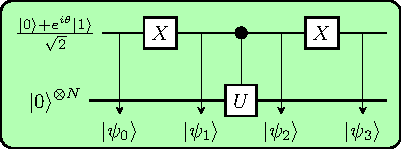
\includegraphics[width=\linewidth]{circuits/circuit1.pdf}
  \caption[Example reduced circuit]{Example circuit that measures $e^{i\theta}\sandwich{0}{\bm U}{0}$ for some unitary matrix $\bm U$ and an angle $\theta$}
  \label{fig:circuitreal}
\end{figure}

To highlight how the circuit evaluates the elements of matrices $\bm M$ and $\bm V$, we refer to a more basic circuit represented in figure \ref{fig:circuitreal}, which evolves as follows:
\begin{equation*}
	\begin{split}
		\ket {\psi_0}
		&= \paren{\frac{\ket 0 + e^{i\theta}\ket 1}{\sqrt 2}}\otimes \ket 0^{\otimes\elec} \\
		\ket {\psi_1}
		&= \paren{\frac{\ket 1 + e^{i\theta}\ket 0}{\sqrt 2}}\otimes \ket 0^{\otimes\elec} \\
		\ket {\psi_2}
		&= \frac{\ket 1}{\sqrt 2} \otimes \bm U \ket 0^{\otimes\elec} + \frac{e^{i\theta}}{\sqrt 2}\ket 0 \otimes \ket 0^{\otimes\elec} \\
		\ket {\psi_3}
		&= \frac{\ket 0}{\sqrt 2} \otimes \bm U \ket 0^{\otimes\elec} + \frac{e^{i\theta}}{\sqrt 2}\ket 1 \otimes \ket 0^{\otimes\elec} \\
		\intertext{\text{We can now change basis to 
		$\ket + = \frac{\ket 0 + \ket 1}{\sqrt 2}$
		and
		$\ket - = \frac{\ket 0 - \ket 1}{\sqrt 2}$:}}
		\psi_3
		&= \frac{\ket + + \ket -}{2} \otimes \bm U \ket 0^{\otimes\elec} + e^{i\theta}\frac{\ket + - \ket -}{2} \otimes \ket 0^{\otimes\elec} \\
		&= \ket + \frac{\bm U + e^{i\theta}\bm I}{2}\ket 0^{\otimes\elec} 
		+ \ket - \frac{\bm U - e^{i\theta}\bm I}{2}\ket 0^{\otimes\elec} 
	\end{split}
\end{equation*}
%
The probability of measuring $\ket +$ on the first qubit is:
%
\begin{equation*}
	\begin{split}
		P(\ket +)
		&= \sandwich 0 {
			\paren{\frac{\bm U + e^{i\theta}\bm I}{2}}
			\paren{\frac{\bm U + e^{i\theta}\bm I}{2}}^\dagger
		} 0 \\
		&= \sandwich 0 {
			\paren{\frac{\bm U + e^{i\theta}\bm I}{2}}
			\paren{\frac{\bm U^\dagger + e^{-i\theta}\bm I}{2}}
		} 0 \\
		&= \sandwich 0 {
			\paren{\frac{\bm U\bm U^\dagger + \bm Ue^{-i\theta}\bm I + \bm U^\dagger e^{i\theta}\bm I + \bm I^2}{4}}
		} 0 \\
		&= \sandwich 0 {
			\paren{\frac{\bm Ue^{-i\theta}\bm I + \bm U^\dagger e^{i\theta}\bm I}{4}}
		} 0 
		+ \frac{\sandwich 0 {\bm I} 0}{2} \\
		&= \sandwich 0 {
			\paren{\frac{\bm Ue^{-i\theta}\bm I + \paren{\bm Ue^{i\theta}\bm I}^\dagger}{4}}
		} 0 
		+ \frac{1}{2} \\
		&= \frac{Re \paren{e^{i\theta}\sandwich 0 { \bm U } 0}}{2}
		+ \frac{1}{2} \\
	\end{split}
\end{equation*}
%
A more involved circuit that uses this principle comes from Li's paper \shortcite{benjamin}, as shown in figure \ref{fig:circuitbenjamin}.
%
\begin{figure}[h!]
  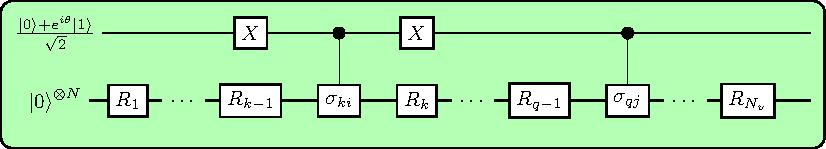
\includegraphics[width=\linewidth]{circuits/circuit2.pdf}
  \caption[Li's circuit]{Li's circuit to measure $a \cdot Re\paren{e^{i\theta}\sandwich 0 {\bm U} 0}$, which is then used to calculate $\bm M_{kq}$ for the \gls{tdvp}. The circuit that calculates $\bm V_k$ is similar, as it simply takes $q = N_v + 1$}
  \label{fig:circuitbenjamin}
\end{figure}
%
The first (topmost) qubit in this circuit evolves into the state:
%
\begin{equation*}
	\begin{split}
		\ket \phi 
		&= \frac{\ket 0}{\sqrt 2} \otimes \bm R_{N_v} \ldots \bm R_k \cdot \bm \sigma_{ki} \cdot \bm R_{k-1} \ldots \bm R_1 \ket 0^{\otimes \elec}\\
		&\quad + \frac{e^{i\theta}\ket 1}{\sqrt 2} \otimes \bm R_{N_v} \ldots \bm R_q \cdot \bm \sigma_{qj} \cdot \bm R_{q-1} \ldots \bm R_1 \ket 0^{\otimes \elec}\\
		\span\text{We can now use \ref{eq:rki} to simplify our expression:}\\
		&= \frac{\ket 0}{\sqrt 2} \otimes \bm R_{ki} \ket 0^{\otimes \elec}
		+ \frac{e^{i\theta}\ket 1}{\sqrt 2} \bm R_{qj}\ket 0^{\otimes \elec}\\
		\span\text{We can now change basis in our first qubit to
		$\ket + = \frac{\ket 0 + \ket 1}{\sqrt 2}$
		and
		$\ket - = \frac{\ket 0 - \ket 1}{\sqrt 2}$:}\\
		&= \frac{\ket + + \ket -}{2} \otimes \bm R_{ki} \ket 0^{\otimes \elec}
		+ \frac{e^{i\theta}\paren{\ket + - \ket -}}{2} \bm R_{qj}\ket 0^{\otimes \elec}\\
		&= \ket + \otimes \frac{\bm R_{ki} + e^{i\theta}\bm R_{qj}}{2} \ket 0^{\otimes \elec}
		 + \ket - \otimes \frac{\bm R_{ki} - e^{i\theta}\bm R_{qj}}{2} \ket 0^{\otimes \elec}
	\end{split}
\end{equation*}
The probability of measuring $\ket +$ on the first qubit is:
\begin{equation*}
	\begin{split}
		P(\ket +)
		&= \sandwich 0 {
			\frac{1}{2}\paren{\bm R_{ki} + e^{i\theta} \bm R_{qj}}
			\frac{1}{2}\paren{\bm R_{ki} + e^{i\theta} \bm R_{qj}}^{\dagger}
		} 0 \\
		&= \frac 1 4 \sandwich 0 {
			\paren{\bm R_{ki} + e^{i\theta} \bm R_{qj}}
			\paren{\bm R_{ki}^\dagger + e^{-i\theta} \bm R_{qj}^{\dagger}}
		} 0 \\
		&= \frac 1 4 \sandwich 0 {
			\bm R_{ki}\bm R_{ki}^\dagger + e^{-i\theta} \bm R_{ki}\bm R_{qj}^{\dagger} 
			+ e^{i\theta} \bm R_{qj}\bm R_{ki}^\dagger + \bm R_{qj}\bm R_{qj}^\dagger
		} 0 \\
		&= \frac 1 4 \sandwich 0 {
			e^{-i\theta} \bm R_{ki}\bm R_{qj}^{\dagger} + \paren{e^{-i\theta} \bm R_{ki}\bm R_{qj}^\dagger}^\dagger
		} 0 
			+ \frac{\sandwich 0 I 0}{2}\\
		&= \frac 1 2 Re\paren{e^{i\theta}\sandwich 0 {
			 \bm R_{ki}\bm R_{qj}^{\dagger}
	} 0 }
			+ \frac{1}{2}\\
	\end{split}
\end{equation*}
The probability of measuring $\ket -$ on the first qubit is then:
\begin{equation*}
	\begin{split}
		P(\ket -)
		= \frac 1 2 - \frac 1 2 Re\paren{e^{i\theta}\sandwich 0 {
			 \bm R_{ki}\bm R_{qj}^{\dagger}
	} 0 }
	\end{split}
\end{equation*}
The average measurement of this circuit is then $Avg = P(\ket +) \cdot 1 + P(\ket -) \cdot (-1) = Re\paren{e^{i\theta}\sandwich 0 {\bm R_{ki}\bm R_{qj}^{\dagger}} 0}$ since the eigenvalue of $\ket +$ is 1 and the eigenvalue of $\ket -$ is -1.
%
Taking $a_{kiqj} = 2\cdot \abs{if_{k, i}^*f_{q, j}}, \theta = \arg \paren{if_{k, i}^*f_{q, j}}$ and referring back to \ref{eq:benjamin}:
\begin{equation*}
	\begin{split}
		\sum_{i, j \in P_\elec} a_{kiqj} \cdot Avg_{kiqj} 
		&= \sum_{i, j \in P_\elec} a_{kiqj}\cdot Re\paren{e^{i\theta}\sandwich 0 {\bm R_{ki}\bm R_{qj}^{\dagger}} 0}\\
		&= \sum_{i, j \in P_\elec} a_{kiqj}\cdot Re\paren{\frac{if_{k, i}^*f_{q, j}}{\abs{if_{k, i}^*f_{q, j}}}\sandwich 0 {\bm R_{ki}\bm R_{qj}^{\dagger}} 0}\\
		&= \sum_{i, j \in P_\elec} \frac{a_{kiqj}}{\abs{if_{k, i}^*f_{q, j}}} Re\paren{if_{k, i}^*f_{q, j}\sandwich 0 {\bm R_{ki}\bm R_{qj}^{\dagger}} 0}\\
		&= \sum_{i, j \in P_\elec} 2 Re\paren{if_{k, i}^*f_{q, j}\sandwich 0 {\bm R_{ki}\bm R_{qj}^{\dagger}} 0}\\
		&= \sum_{i, j \in P_\elec} 
		\left [if_{k, i}^*f_{q, j}\sandwich 0 {\bm R_{ki}\bm R_{qj}^{\dagger}} 0 +
		\paren{if_{k, i}^*f_{q, j}\sandwich 0 {\bm R_{ki}\bm R_{qj}^{\dagger}} 0}^* \right ]\\
	\end{split}
\end{equation*}
%
That is, we can calculate $\bm M_{kq}$ as a weighted sum of the average measurement of the circuits for each pair $k, q$, where the products $a_{kiqj} = 2\cdot \abs{if_{k, i}^*f_{q, j}}$ are the weights.
Similarly, $\bm V_k$ can be calculated as a weighted sum where the products $a_{kij} = 2\cdot \abs{f_{k, i}^*h_j}$ are the weights.

Using our evaluation of $\ket\Psi$ in terms of $\rho_\ind 0, \rho_\ind 1, \omega_\ind 0, \omega_\ind 1$, we obtained 
$\bm R = 
\bm R_6(\omega_\ind 0) \cdot
\bm R_5(\omega_\ind 1) \cdot
\bm R_4(\rho_\ind 0) \cdot
\bm R_3(\rho_\ind 1) \cdot
\bm R_2(\omega_\ind 0) \cdot
\bm R_1(\omega_\ind 1)
$, through Eq. \ref{eq:rdecomposition}.
%
We then used the matrices $\bm R_k$ to find our coefficients $f_{k, i} \in \mathbb{C}$ via \ref{eq:r_to_f}. Finally, for each pair of nonzero coefficients $f_{k, i}, f_{q, j}$ we can assemble a circuit and measure its average to obtain $\bm M_{kq}$ gates used in, for example, circuit \ref{fig:circuit}.

%-------------------------------------------------------------------------------------

\section {\textbf{Circuit for 1-electron model}}

The 1-electron case is somewhat simpler than the 2-electron counterpart. We follow through the same steps, however. We must get an expression for $\ket \Psi$, use it to obtain a matrix $\bm R$, decompose it into a product of single-variable matrices $\bm R_k$ and use these to find our $f$ coefficients. Then we must find the Hamiltonian $\hat H$ and use it to find the $h$ coefficients. Using the $f$ and $h$ coefficients, we can assemble a circuit.
%
\subsection {\textbf{Dynamics}}
%
We take somewhat similar steps to before in solving the lagrangian. Taking a look at our previous decomposition of $\bm u$ through \ref{eq:udecomposition} and \ref{eq:urotation}:
\begin{equation*}
\begin{split}
	\ket\Psi 
	= \bigotimes_{\ind 0} 
		\bm u_{\lambda_{\ind 0}} \ket 0
	= \bigotimes_{\ind 0} 
		\bm R_z(\omega_{\ind 0}) \bm R_y(2\rho_\ind 0) \bm R_z(-\omega_\ind 0) \ket 0
	= \bm R_z(\omega) \bm R_y(2\rho) \bm R_z(-\omega) \ket 0
\end{split}
\end{equation*}
%
Meaning we have two variables $\omega$ and $\rho$. Let $\omega$ be $\lambda_1$ and $\rho$ be $\lambda_2$. Therefore, we have:
%
\begin{equation*}
	\begin{split}
		L &= \frac{i}{2}\bra{\Psi}{\kpp t} - \frac{i}{2}{\bpp{t}}\ket{\Psi} - \sandwich{\Psi}{\hat H}{\Psi} \\
	L &= 	
		\sum_j \frac{i}{2}\bra{\Psi}{\kpp {\lambda_j}} \dot \lambda_j
	- 	\sum_j \frac{i}{2}{\bpp{\lambda_j}}\ket{\Psi}\dot{\lambda_j}
	- \sandwich{\Psi}{\hat H}{\Psi}
	\end{split}
\end{equation*}
%
Taking the derivative of $L$ with regards to $\lambda_k$ for $k \in \{1, 2\}$:
%
\begin{equation*}
	\begin{split}
	\pd{\lambda_k} L &= 	
	\phantom{-}\sum_j \frac{i}{2}\bra{\Psi}{\kppd {\lambda_k}{\lambda_j}} \dot \lambda_j
	+	\sum_j \frac{i}{2}\bpp{\lambda_k}{\kpp {\lambda_j}} \dot \lambda_j \\
	&\quad -\sum_j \frac{i}{2}{\bppd{\lambda_k}{\lambda_j}}\ket{\Psi}\dot{\lambda_j}
	- 	\sum_j \frac{i}{2}{\bpp{\lambda_j}}\kpp{\lambda_k}\dot{\lambda_j}\\
	&\quad -\pd{\lambda_k} \sandwich{\Psi}{\hat H}{\Psi}
	\end{split}
\end{equation*}
%
Taking the derivative of $L$ with regards to $\dot{\lambda_k}$ for $k \in \{1, 2\}$:
%
\begin{equation*}
	\begin{split}
		\pd{\dot{\lambda_k}} L &=
		\frac{i}{2}\bra{\Psi}{\kpp {\lambda_k}}
	- 	\frac{i}{2}{\bpp{\lambda_k}}\ket{\Psi}
	\end{split}
\end{equation*}
%
Taking the derivative of the expression above with regards to time:
%
\begin{equation*}
	\begin{split}
		\ddt \pd{\dot{\lambda_k}} L &=
		\sum_j \frac{i}{2}\bpp{\lambda_j}{\kpp {\lambda_k}} \dot \lambda_j
	+	\sum_j \frac{i}{2}\bra{\Psi}{\kppd {\lambda_j}{\lambda_k}} \dot \lambda_j \\
    	&- 	\sum_j \frac{i}{2}{\bppd{\lambda_j}{\lambda_k}}\ket{\Psi}\dot{\lambda_j}
	- 	\sum_j \frac{i}{2}{\bpp{\lambda_k}}\kpp{\lambda_j}\dot{\lambda_j}
	\end{split}
\end{equation*}
%
Now, since the Euler-Lagrange equation gives us $\pd{\lambda_k} L = \ddt \pd{\dot {\lambda_k}} L$, the only terms that do not cancel out are as follows:
%
\begin{equation*}
	\begin{split}
		\ddt \pd{\dot{\lambda_k}} L 
	&=	\pd{\lambda_k} L
	\\
	 	\sum_j i \bpp{\lambda_k} \kpp{\lambda_j}\dot{\lambda_j}
	-	\sum_j i \bpp{\lambda_j} \kpp{\lambda_k}\dot{\lambda_j}
	&= 	\pd{\lambda_k}\sandwich{\Psi}{\hat H}{\Psi}
	\end{split}
\end{equation*}
%
This can be written in matrix notation:
%
\begin{equation*}
	\begin{split}
	 	i \left [ \bpp{\lambda_k} \kpp{\lambda_q} 
			- \bpp{\lambda_q} \kpp{\lambda_k} \right ]_{kq}
		\cdot \left[ \dot \lambda_q \right]_q
	&= 	\left[\pd{\lambda_k}\sandwich{\Psi}{\hat H}{\Psi}\right]_k \\
	\begin{pmatrix}
		0 & i \bpp{\lambda_1} \kpp{\lambda_2} - i \bpp{\lambda_2} \kpp{\lambda_1} \\
		i \bpp{\lambda_2} \kpp{\lambda_1} - i \bpp{\lambda_1} \kpp{\lambda_2} & 0
	\end{pmatrix} 
	\begin{pmatrix}
		\dot \lambda_1 \\
		\dot \lambda_2 
	\end{pmatrix} 
	    &=
	\begin{pmatrix}
		\pd {\lambda_1} \sandwich{\Psi}{\hat H}{\Psi}\\
		\pd {\lambda_2} \sandwich{\Psi}{\hat H}{\Psi}\\
	\end{pmatrix} \\
	\sum_q M_{kq} \dot \lambda_q = V_k
	\end{split}
\end{equation*}
%
Where:
\begin{equation*}
	\begin{split}
	M_{kq} 
	&= 
	 	i \bpp{\lambda_k} \kpp{\lambda_q} - i \bpp{\lambda_q} \kpp{\lambda_k} 
	\\
	V_k 
	&= 	\pd{\lambda_k}\sandwich{\Psi}{\hat H}{\Psi} \\
	\end{split}
\end{equation*}
%
Taking a look at our previous decomposition of $\bm u$ through Eq. \ref{eq:psirw}, we can find our wavefunction $\ket\Psi$:
%
\begin{equation*}
	\begin{split}
	\ket \Psi 
	&= \bm u_{\lambda_\ind 0} \ket {\psi_{\oo 0}} \\
	&= \co {\rho} \ket {\psi_{\oo 0}} + \s {\rho}e^{i\omega} \ket{\psi_{\uo 0}} \\
	\end{split}
\end{equation*}
%
We can now calculate the elements of $\bm M$. First we calculate the values of the derivatives of $\ket \Psi$ with respect to $\rho$ and $\omega$.
%
\begin{equation*}
	\begin{split}
		\ket{\Psi} 
		&= \co{\rho}\ket{\psi_{\oo {0}}} + \s\rho e^{i\omega}\ket{\psi_{\uo {0}}} 
		%
		\\
		%
		\pd\omega\ket\Psi 
		&= \co\rho\ket{\psi_{\oo {0}}} + i\s\rho e^{i\omega}\ket{\psi_{\uo {0}}} 
		%
		\\
		%
		\pd\rho\ket\Psi 
		&= -\s\rho\ket{\psi_{\oo {0}}} + \co\rho e^{i\omega}\ket{\psi_{\uo {0}}} 
	\end{split}
\end{equation*}

Then we get the dual $\bra\Psi = {\ket\Psi}^\dagger$ and calculate its derivatives:
\begin{equation*}
	\begin{split}
		\bra{\Psi} 
		&= \co{\rho}\bra{\psi_{\oo {0}}} + \s\rho e^{-i\omega}\bra{\psi_{\uo {0}}}
		%
		\\
		%
		\pd\omega\bra\Psi 
		&= \co\rho\bra{\psi_{\oo {0}}} - i\s\rho e^{-i\omega}\bra{\psi_{\uo {0}}}
		%
		\\
		%
		\pd\rho\bra\Psi 
		&= -\s\rho\bra{\psi_{\oo {0}}} + \co\rho e^{-i\omega}\bra{\psi_{\uo {0}}}
	\end{split}
\end{equation*}
%
Finally:
%
\begin{equation*}
	\begin{split}
	i \bpp{\omega} \kpp{\rho} - i \bpp{\rho} \kpp{\omega} 
	&= 
	i\paren{-\s\rho\co\rho - i\s\rho\co\rho} \\
	&\quad 
	-i\paren{-\s\rho\co\rho + i\s\rho\co\rho} \\
	&=
	i\paren{-2i\s\rho\co\rho} \\
	&=
	\s{2\rho}
	%
	\\
	%
	i \bpp{\rho} \kpp{\omega} - i \bpp{\omega} \kpp{\rho} 
	&= 
	- \paren{i \bpp{\omega} \kpp{\rho} - i \bpp{\rho} \kpp{\omega}} \\
	&=
	-\s{2\rho}
	\end{split}
\end{equation*}
%
And we have the values for the $\bm M$ matrix:
%
\begin{equation*}
	\begin{split}
		\bm M = 
	\begin{pmatrix}
		0 & \s{2\rho} \\
		-\s{2\rho} & 0
	\end{pmatrix} 
	\end{split}
\end{equation*}
\begin{equation*}
	\begin{split}
	\begin{pmatrix}
		0 & \s{2\rho} \\
		-\s{2\rho} & 0
	\end{pmatrix} 
	\cdot
	\begin{pmatrix}
		\dot \lambda_1 \\
		\dot \lambda_2 
	\end{pmatrix} 
	    &=
	\begin{pmatrix}
		\pd {\lambda_1} \sandwich{\Psi}{\hat H}{\Psi}\\
		\pd {\lambda_2} \sandwich{\Psi}{\hat H}{\Psi}\\
	\end{pmatrix} \\
	\bm M \dot {\bm \lambda} = \bm V
	\end{split}
\end{equation*}
%
\subsection {\textbf{Wavefunction decomposition}}
Now we need to write $\ket \Psi = \bm R \ket 0 = \prod_{k=N_v}^1 \bm R_k(\lambda_k) \ket 0$ for some integer $N_v$. That is, we need to find a product of matrices of a single variable that, when applied to the ground state, gives us our wavefunction.
For our case where $\elec = 1$ and $\orb = 2$, we have:
%
\begin{equation*}
\begin{split}
	\ket\Psi 
	&= \bm u_{\lambda_{\ind 0}} \ket 0 \\
	&= \bm R_z(\omega) \bm R_y(2\rho) \bm R_z(-\omega)
	\ket 0 \\
	&= 
	\begin{bmatrix}
		e^{-\frac{i\omega} 2} & 0 \\
		0 & e^{\frac{i\omega} 2}\\
	\end{bmatrix} 
	\begin{bmatrix}
		\co \rho & - \s \rho \\
		\s \rho  & \co \rho\\
	\end{bmatrix} 
	\begin{bmatrix}
		e^{\frac{i\omega} 2} & 0 \\
		0 & e^{-\frac{i\omega} 2}\\
	\end{bmatrix} 
	\ket 0 \\
	&=
	\begin{bmatrix}
		\co \rho & - \s \rho e^{-i\omega} \\
		\s \rho e^{i\omega} & \co \rho\\
	\end{bmatrix} 
	\ket 0 \\
	&= \bm R\ket 0
\end{split}
\end{equation*}
%
We can then write the matrix $\bm R$ as a product of 3 matrices. Taking $\lambda_1 = \lambda_3 = \omega$ and $\lambda_2 = \rho$:
%
\begin{equation}
	\begin{split}
	\label{eq:rdecomposition1e}
	\bm R &= \begin{bmatrix}
		\co {\lambda_2} & - \s {\lambda_2} e^{-i{\lambda_1}} \\
		\s {\lambda_2} e^{i{\lambda_1}} & \co {\lambda_2}\\
	\end{bmatrix} \\
	\bm R_3({\lambda_1})  &=
	\begin{bmatrix}
		e^{-\frac{i{\lambda_3}} 2} & 0 \\
		0 & e^{\frac{i{\lambda_3}} 2}\\
	\end{bmatrix} \\
	\bm R_2({\lambda_2}) &= 
	\begin{bmatrix}
		\co {\lambda_2} & - \s {\lambda_2} \\
		\s {\lambda_2}  & \co {\lambda_2}\\
	\end{bmatrix} \\
	\bm R_1({\lambda_1}) &=
	\begin{bmatrix}
		e^{\frac{i{\lambda_1}} 2} & 0 \\
		0 & e^{-\frac{i{\lambda_1}} 2}\\
	\end{bmatrix} \\
	\end{split}
\end{equation}
%
We note here that the order of the operators in \ref{eq:rdecomposition1e} is important, as the matrix $\bm R_2$ does not commute with the others. Thus, we fix the variables 
$\lambda_1 = \omega;  \lambda_2 = \rho; \lambda_3 = \omega$.
%
%
\subsection {\textbf{Obtaining derivative coefficients}}
%
Now that we have each matrix $\bm R_k$, we obtain the decomposition of their derivatives $\fpd{\bm R_k}{\lambda_k}$ into Pauli matrices according to the following equation \cite{benjamin}:
%
\begin{equation}\label{eq:r_to_f1e}
\begin{split}
	\fpd{\bm R_k}{\lambda_k} = \sum_{i \in \{\bm I, \bm X, \bm Y, \bm Z\}} f_{k, i} \bm R_k \bm \sigma_{k, i}
\end{split}
\end{equation}
%
Where $\bm \sigma_{k, i} = i \in \{\bm I, \bm X, \bm Y, \bm Z\}$ are Pauli matrices.
Now we need to determine the coefficients $f_{k, i}$ for every $k \in \{1, 2, 3\}$ and $i \in \{\bm I, \bm X, \bm Y, \bm Z\}$. We accomplish this task by taking a look at \ref{eq:r_to_f1e} for each $k$:
%
\begin{enumerate}
\item $k = 1$:
\begin{align*}
	\frac {d\bm R_1}{d\lambda_1} 
	&= \frac {d\bm R_1}{d\omega} 
	= 
	\begin{bmatrix} 
		\frac i 2 e^{\frac{i\omega} 2} & 0 \\
		0 & -\frac i 2 e^{-\frac{i\omega} 2}\\
	\end{bmatrix}\\
	&= \sum_{\bm A \in \{\bm I, \bm X, \bm Y, \bm Z\}}
		f_{1, \bm A}\bm R_1 \cdot \bm A
		\intertext{The only relevant matrices are $\bm {I}$ and $\bm {Z}$, as the other matrices have only zeroes in the main diagonal.}
	%
	&= f_{1, \bm {I}} \bm R_1 \bm {I}
	+ f_{1, \bm {Z}} \bm R_1 \bm {Z}
	\\
	&= f_{1, \bm {I}}
	\begin{bmatrix} 
		\frac i 2 e^{\frac{i\omega} 2} & 0 \\
		0 & -\frac i 2 e^{-\frac{i\omega} 2}\\
	\end{bmatrix}
	\I
	\\
	&+ f_{1, \bm {Z}}
	\begin{bmatrix} 
		\frac i 2 e^{\frac{i\omega} 2} & 0 \\
		0 & -\frac i 2 e^{-\frac{i\omega} 2}\\
	\end{bmatrix}
	\Z
	\\
	\intertext{The solution to this system is:}
	%
	&= 0 \bm R_1 \paren{\bm {I}} 
	+ \frac i 2 \bm R_1 \paren{\bm {Z}} \\
	&= \frac i 2 \bm R_1 \paren{\bm {Z}}
\end{align*}
%
Li \shortcite{benjamin} states that:
\begin{equation}
	\begin{split}
	\label{eq:rki1e}
	\fpd {\ket \Psi} {\lambda_k} &= \sum_{\bm A \in \{\bm I, \bm X, \bm Y, \bm Z\}}f_{k, \bm A}\bm R_{k, \bm A}\ket 0
	%
	\intertext{\text{Where}}
	%
	\bm R_{k,\bm A} &= \bm R_{N_v} \ldots \bm R_k \cdot \bm A \cdot \bm R_{k - 1} \ldots \bm R_1
\end{split}
\end{equation}
%
So we have:
%
\begin{align*}
	\fpd {\ket\Psi}{\lambda_1} &= \fpd {\ket\Psi}{\omega} = \left[ 
		i \s \rho \co \omega\bm  X + i \s \rho \s \omega\bm  Y
	\right ] \ket 0 \\
	&= \left( 
		i \s \rho \co \omega \X + i \s \rho \s \omega \Y
	\right ) \ket 0 \\
	&= \left( 
		\begin{bmatrix}
			0 & i \s \rho \paren{\co \omega - i \s \omega} \\
			i \s \rho \paren{\co \omega + i \s \omega} & 0\\
		\end{bmatrix}
	\right ) \ket 0 \\
	&= \left( 
		\begin{bmatrix}
			0 & i \s \rho e^{-i\omega} \\
			i \s \rho e^{i\omega} & 0\\
		\end{bmatrix}
	\right ) \ket 0 \\
\end{align*}
%
with Eq. \ref{eq:rki1e}:
%
\begin{align*}
	\bm R_{1, Z} = \bm R_3 \bm R_2 \bm R_1 \sigma_{1, Z} &=
	\bm RZ\\ 
	&= \begin{bmatrix}
		\co \rho & - \s \rho e^{-i\omega} \\
		\s \rho e^{i\omega} & \co \rho\\
	\end{bmatrix} 
	\begin{bmatrix}1 & 0 \\ 0 & -1\end{bmatrix}\\
	&= \begin{bmatrix}
		\co \rho &  \s \rho e^{-i\omega} \\
		\s \rho e^{i\omega} & -\co \rho\\
	\end{bmatrix} 
	\\
\end{align*}
%
and we can see
%
$$
	\sum_{\bm A} f_{1, \bm A} \bm R_{1, \bm A} \ket 0
	= 
	\frac i 2
	\begin{bmatrix}
		\co \rho &  \s \rho e^{-i\omega} \\
		\s \rho e^{i\omega} & -\co \rho\\
	\end{bmatrix}
	\neq \fpd{\ket\Psi}{\omega}
$$
This happens since our variables aren't unique. In this case, $\lambda_1 = \lambda_5$, and we'll see later that Li's \shortcite{benjamin} Eq. \ref{eq:rki1e} needs to be corrected in our approach to include terms that use the same variable:
%
\begin{equation}
	\begin{split}
		\label{eq:correctedli1e}
	\fpd{\ket\Psi}{\lambda_k}
	=\sum_{j:\lambda_k = \lambda_j} \sum_{\bm A \in P_\elec} f_{j, \bm A} \bm R_{j, \bm A} \ket 0 
	\end{split}
\end{equation}

\item $k = 2$

\begin{align*}
	\frac {d\bm R_2}{d\lambda_2} 
	&= \frac {d\bm R_2}{d\omega} 
	=
	\begin{bmatrix}
		-\s \rho & - \co \rho \\
		\co \rho & -\s \rho\\
	\end{bmatrix} \\
	&= \sum_{\bm A \in \{\bm I, \bm X, \bm Y, \bm Z\}} f_{2, \bm A} \bm R_2 \cdot \bm A 
	\intertext{This time, the relevant matrices in $\{\bm I, \bm X, \bm Y, \bm Z\}$ are $\bm {Y}$ and $\bm {X}$:}
	%\\
	&= f_{2, \bm {Y}} \bm R_2 \paren{\bm {Y}} 
	+ f_{2, \bm {X}} \bm R_2 \paren{\bm {X}} 
	\\
	&= f_{2, \bm {Y}}
	\begin{bmatrix}
		\co {\rho} & - \s {\rho} \\
		\s {\rho}  & \co {\rho}\\
	\end{bmatrix} 
	\Y
	\\
	&+ f_{2, \bm {X}}
	\begin{bmatrix}
		\co {\rho} & - \s {\rho} \\
		\s {\rho}  & \co {\rho}\\
	\end{bmatrix} 
	\X
	\\
	\intertext{The solution to this system is:}
	%\\
	&= -i \bm R_2 \paren{\bm {Y}} 
	+ 0 \bm R_2 \paren{\bm {X}} \\
	&= -i \bm R_2 \paren{\bm {Y}} 
\end{align*}
%
This time, Li's \shortcite{benjamin} Eq. \ref{eq:rki1e} is satisfied by our result:
%
\begin{align*}
	\fpd {\ket\Psi}{\lambda_2} 
	&= \fpd {\ket\Psi}{\rho}
	= 
	\left[ 
		- \s \rho \bm I + i \co \rho \s \omega \bm X - i \co \rho \co \omega\bm Y
	\right ] \ket 0 \\
	&=
	\left[ 
		- \s \rho \I + i \co \rho \s \omega \X - i \co \rho \co \omega \Y
	\right ] \ket 0 \\
	&=
		\begin{bmatrix}
			- \s \rho & \co \rho \paren{i\s \omega - \co \omega} \\
			\co \rho \paren{ i\s \omega + \co \omega} & -\s \rho
		\end{bmatrix}
	\ket 0 \\
	&=
		\begin{bmatrix}
			- \s \rho & -\co \rho e^{-i\omega} \\
			\co \rho e^{i\omega} & -\s \rho
		\end{bmatrix}
	\ket 0 \\
\end{align*}
%
with Eq. \ref{eq:rki1e}:
%
\begin{align*}
	\bm R_{2, \bm {Y}} &= \bm R_3 \bm R_2 \paren{\bm {Y}} \bm R_1 \\
	&= \begin{bmatrix}e^{-\frac{i}{2}\omega} & 0 \\ 0 & e^{\frac i 2\omega}\end{bmatrix}
	\begin{bmatrix}
		\co \rho & - \s \rho \\
		\s \rho & \co \rho\\
	\end{bmatrix} 
	\Y 
	\begin{bmatrix}e^{\frac{i}{2}\omega} & 0 \\ 0 & e^{-\frac i 2\omega}\end{bmatrix}\\
	&=
	\begin{bmatrix}
		e^{-\frac i 2\omega}\co \rho & - e^{-\frac i 2\omega}\s \rho \\
		e^{\frac i 2\omega}\s \rho & e^{\frac i 2\omega}\co \rho\\
	\end{bmatrix} 
	\begin{bmatrix}0 & -ie^{-\frac i 2\omega} \\ ie^{\frac i 2\omega} & 0\end{bmatrix}\\
	&= \begin{bmatrix}
		-i \s \rho & -ie^{-i\omega} \co \rho \\
		ie^{i\omega} \co \rho & -i\sin \rho\\
	\end{bmatrix} 
\end{align*}
%
and we can see
$$
	\sum_{\bm A \in \{\bm I, \bm X, \bm Y, \bm Z\}} f_{2, \bm A} \bm R_{2, \bm A} \ket 0 
	= -i \bm R_{2, \bm Y}
	= \fpd{\ket\Psi}{\omega}
$$
%
As expected, since our $\lambda_2$ variable is unique in our set of variables.
%
\item $k = 3$
%
\begin{align*}
	\frac {d\bm R_3}{d\lambda_3} 
	&= \frac {d\bm R_3}{d\omega} 
	=
	\begin{bmatrix}
		- \frac i 2 e^{-\frac {i\omega} 2} & 0 \\
		0 &  \frac i 2 e^{\frac {i\omega} 2}
	\end{bmatrix}\\
	&= \sum_{\bm A \in \{\bm I, \bm X, \bm Y, \bm Z\}} f_{3, \bm A} \bm R_3 \cdot \bm A 
	\intertext{The relevant matrices in $\{\bm I, \bm X, \bm Y, \bm Z\}$ are $\bm {I}$ and $\bm {Z}$:}
	%
	&= f_{3, \bm {I}} 
	\begin{bmatrix}
		e^{-\frac{i{\omega}} 2} & 0 \\
		0 & e^{\frac{i{\omega}} 2}\\
	\end{bmatrix} 
	\I
	+ f_{3, \bm {Z}} 
	\begin{bmatrix}
		e^{-\frac{i{\omega}} 2} & 0 \\
		0 & e^{\frac{i{\omega}} 2}\\
	\end{bmatrix} 
	\Z
	\\
	\intertext{The solution to this system is:}
	%\\
	&= 0 \bm R_3 \paren{\bm {I}}
	- \frac i 2 \bm R_3 \paren{\bm {Z}} \\
	&= -\frac i 2 \bm R_3 \paren{\bm {Z}}
\end{align*}
%
Looking at Li's \shortcite{benjamin} Eq. \ref{eq:rki} again, we have:
%
\begin{align*}
	\fpd {\ket\Psi}{\lambda_3} &= \fpd {\ket\Psi}{\omega} = \left[ 
		i \s \rho \co \omega\bm  X + i \s \rho \s \omega\bm  Y
	\right ] \ket 0 \\
	&= \left( 
		i \s \rho \co \omega \X + i \s \rho \s \omega \Y
	\right ) \ket 0 \\
	&= \left( 
		\begin{bmatrix}
			0 & i \s \rho \paren{\co \omega - i \s \omega} \\
			i \s \rho \paren{\co \omega + i \s \omega} & 0\\
		\end{bmatrix}
	\right ) \ket 0 \\
	&= \left( 
		\begin{bmatrix}
			0 & i \s \rho e^{-i\omega} \\
			i \s \rho e^{i\omega} & 0\\
		\end{bmatrix}
	\right ) \ket 0 
\end{align*}
%
with Eq. \ref{eq:rki1e}:
%
\begin{align*}
	\bm R_{3, \bm {Z}} &= \bm R_3 \paren{\bm {Z}} \bm R_2 \bm R_1
	\\
	&=\begin{bmatrix}
		e^{-\frac {i\omega} 2} & 0 \\
		0 & e^{\frac {i\omega} 2}
	\end{bmatrix} 
	\Z R_2 R_1
	\\
	&=\begin{bmatrix}
		e^{-\frac {i\omega} 2} & 0 \\
		0 & -e^{\frac {i\omega} 2}
	\end{bmatrix} 
	R_2 R_1
	= Z R_3 R_2 R_1
	\\
	&= \begin{bmatrix}1 & 0 \\ 0 & -1\end{bmatrix}
	\begin{bmatrix}
		\co \rho & - \s \rho e^{i\omega} \\
		\s \rho e^{i\omega} & \co \rho\\
	\end{bmatrix} 
	\\
	&= \begin{bmatrix}
		\co \rho &  -\s \rho e^{i\omega} \\
		-\s \rho e^{i\omega} & -\co \rho\\
	\end{bmatrix} 
\end{align*}
%
and we can see
%
$$
	\sum_{\bm A \in \{\bm I, \bm X, \bm Y, \bm Z\}} f_{3, \bm A} \bm R_{3, \bm A} \ket 0 
	\neq \fpd{\ket\Psi}{\rho_\ind 1}
$$
%
Using the Eq. \ref{eq:correctedli1e}, however, we can verify:
%
$$
	\sum_{\bm A \in \{\bm I, \bm X, \bm Y, \bm Z\}} f_{1, \bm A} \bm R_{1, \bm A} \ket 0 
	+ \sum_{\bm A \in \{\bm I, \bm X, \bm Y, \bm Z\}} f_{3, \bm A} \bm R_{3, \bm A} \ket 0 
	= \fpd{\ket\Psi}{\omega}
	= \fpd{\ket\Psi}{\lambda_1}
	= \fpd{\ket\Psi}{\lambda_3}
$$
%
As expected since $\lambda_3 = \lambda_1$.
%
\end{enumerate}
%
Now we have the coefficients $f_{k, i}$ that are not zero:
%
\begin{equation*}
	\begin{split}
		f_{1, \bm {Z}} &= \frac i 2 \\
		f_{2, \bm {Y}} &= -i \\
		f_{3, \bm {Z}} &= -\frac i 2 \\
	\end{split}
\end{equation*}
%
Which means the only relevant Pauli matrices for this case are:
%
\begin{align*}
	\bm Y, \bm Z
\end{align*}

\subsection{\textbf{Hamiltonian and potential matrix for 1 electron}}

Our potential matrix, $V$ is:
%
\begin{equation*}
	\begin{split}
		V = \begin{pmatrix}
			\pd {\lambda_1} \sandwich {\Psi}{\hat H}{\Psi}\\
			\pd {\lambda_2} \sandwich {\Psi}{\hat H}{\Psi}\\
		\end{pmatrix}
	\end{split}
\end{equation*}
%
To calculate that, we first need our hamiltonian $\hat H$ and $\ket \Psi$. To calculate the Hamiltonian, we refer back to equations \ref{eq:electronhamiltonian} and \ref{eq:electronhamiltonianaux}. Fortunately, since there's only one electron, we can safely disregard the electron interaction:
%
\begin{equation*}
	\begin{split}
	\hat H  &= \sum_{\go 0, \go 1}h_{\go 0 \go 1}\creg 0 \anig 1 \\
		&= {h_{\alpha\alpha}} \creo 0 \anio 0
		+ {h_{\mu\mu}} \creu 0 \aniu 0
		+ h_{\mu\alpha} \creu 0 \anio 0 
%
		\\
%
		&= \frac{h_{\alpha\alpha}}{2} \paren{\hat I + \hat Z}
		+ \frac{h_{\mu\mu}}{2} \paren{\hat I - \hat Z}
		+ h_{\mu\alpha} \hat X
%
	\\
%
		&= 	\frac{1}{2} \left[ 
			\paren{h_{\alpha\alpha} + h_{\mu\mu}} \hat I 
		+	\paren{h_{\alpha\alpha} - h_{\mu\mu}} \hat Z
		+ 	2 \cdot h_{\mu\alpha} \hat X
	\right]
%
	\\
%
		&=	h_{I} \cdot \hat I 
		+	h_{Z} \cdot \hat Z
		+	h_{X} \cdot \hat X
	\end{split}
\end{equation*}
%
Where:
%
\begin{equation*}
	\begin{split}
			h_{I}
		&=	\frac{h_{\alpha\alpha} + h_{\mu\mu}} 2
%
	\\
%
			h_{Z}
		&=	\frac{h_{\alpha\alpha} - h_{\mu\mu}} 2
%
	\\
%
			h_{X}
		&= 	h_{\mu\alpha}
%
	\end{split}
\end{equation*}
%
We also have the values of
$
h_{\alpha\alpha}, h_{\mu\mu}, h_{\mu\alpha}$
for a Hydrogen atom. They're tabled values, and under STO-3G basis set (Approximates the Slater type orbitals by the use of three Gaussian curves), these values can be found in \shortcite{szabo}:
\begin{equation*}
	\begin{split}
		h_{\alpha\alpha} &= -1.2528 \text{ a.u.} \\
		h_{\mu\mu} &= -0.4756 \text{ a.u.}\\
		h_{\mu\alpha} &= 0 \text{ a.u.}
	\end{split}
\end{equation*}
%
We now need to calculate $\sandwich{\Psi}{\hat H}{\Psi}$ and for that we shall use:
%
\begin{equation*}
	\begin{split}
		\hat H 
		&= \frac{h_{\alpha\alpha}}{2} \paren{\hat I + \hat Z}
		+ \frac{h_{\mu\mu}}{2} \paren{\hat I - \hat Z} 
		+ h_{\mu\alpha} \hat X\\
		\ket \Psi 
		&= \co \rho \ket 0 + e^{i \omega} \s \rho \ket 1 \\
		\bra \Psi 
		&= \bra 0 \co \rho  + \bra 1 e^{-i \omega} \s \rho 
	\end{split}
\end{equation*}
%
Therefore:
%
\begin{equation*}
	\begin{split}
		\sandwich \Psi {\hat H} \Psi
		&= \bra \Psi \frac 1 2 \left[
			h_{\alpha\alpha} (\hat I + \hat Z) \paren{\co \rho \ket 0 + \s \rho e^{i\omega} \ket 1} \right .\\
		& \quad + h_{\mu\mu} (\hat I - \hat Z) \paren{\co \rho \ket 0 + \s \rho e^{i\omega} \ket 1} \\
		&\left. \quad + 2 h_{\mu\alpha} \hat X \paren{\co \rho \ket 0 + \s \rho e^{i\omega} \ket 1}
		\right] \\
		&= \bra \Psi \frac 1 2 \left(
			2h_{\alpha\alpha} \co \rho \ket 0 + 2h_{\mu\mu} \s \rho e^{i\omega} \ket 1
			+ 2h_{\mu\alpha} \paren{\co \rho \ket 1 + \s \rho e^{i\omega} \ket 0}
		\right) \\
		&= \bra \Psi \left(
			h_{\alpha\alpha} \co \rho \ket 0 + h_{\mu\mu} \s \rho e^{i\omega} \ket 1
			+ h_{\mu\alpha} \paren{\co \rho \ket 1 + \s \rho e^{i\omega} \ket 0}
		\right) \\
		&= \paren{\bra 0 \co \rho  + \bra 1 e^{-i \omega} \s \rho } \\
		& \quad \times \left (
			h_{\alpha\alpha} \co \rho \ket 0 + h_{\mu\mu} \s \rho e^{i\omega} \ket 1
			+ h_{\mu\alpha} \paren{\co \rho \ket 1 + \s \rho e^{i\omega} \ket 0}
		\right) \\
		&= \braket 0 0 \co \rho h_{\alpha\alpha} \co \rho 
		+ \braket 1 1 e^{-i \omega} \s \rho h_{\mu\mu} \s \rho e^{i\omega} \\
		&\quad + h_{\mu\alpha} \paren{\co \rho e^{-i \omega} \s \rho \braket 1 1 + \s \rho e^{i\omega} \co \rho \braket 0 0} \\
		&=  h_{\alpha\alpha} \co \rho ^2
		+ h_{\mu\mu} \s \rho ^2
		+ h_{\mu\alpha} \co \omega \s {2\rho}\\
	\end{split}
\end{equation*}
%
Finally,
%
\begin{equation*}
	\begin{split}
		V = \begin{pmatrix}
			- h_{\mu\alpha} \s \omega \s {2\rho} \\
			(h_{\mu\mu} - h_{\alpha\alpha}) \s {2\rho}
			+ 2h_{\mu\alpha} \co \omega \co {2\rho}
		\end{pmatrix}
	\end{split}
\end{equation*}
%
Now each individual term of $\bm M$ and $\bm V$ can be rewritten in terms of our newfound variables using \ref{eq:benjamin}.
%
Each term in \ref{eq:benjamin} can be written as $a\operatorname{Re}\paren{e^{i\theta}\sandwich 0 U 0}$, with real parameters $a$ and $\theta$, and there is a quantum circuit that can efficiently evaluate it.
%
%-------------------------------------------------------------------------------------
%

% Lucas, why is it only initial results? This makes it seem like this is a proposal not a dissertation. 
% Chapter 5 seems much too brief. 
% You also need to clearly and succinctly note your key contributions, I am not seeing that anyonwhere. 

\chapter{\textbf{Results and Future Directions}}\label{chap:results}

\section{\textbf{Contributions}}
Using Fukutome's \shortcite{fukutome} unitary approach to the \gls{hf} method, we've obtained a reference wavefunction $\ket \Psi(\bm \omega, \bm \rho) = \hat U\ket 0$ that depends on vectors of real rotation angles $\bm \omega$ and $\bm \rho$. 

We've then added on Fukutome's work by applying some approximations to obtain a wavefunction with operators that act on single electrons, described by \ref{eq:udecomposition}. These were instrumental in obtaining a simpler wavefunction that fit our generalization of Li's circuit \shortcite{benjamin}.

Next, we've solved the Euler-Lagrange differential equation system related to that wavefunction to get an algebraic result for the matrices in our system.
We've then decomposed $\hat U$ into a product of matrices that depend on a single variable $\hat U = \prod_{\ind 0} \bm R(\lambda_{\ind 0})$, a step necessary to build our \gls{qc}.

We've then adapted the construction of the circuit from Li \shortcite{benjamin} to cater to our reduced set of variables and developed circuits to calculate each of the elements of the matrices $\bm M$ and $\bm V$ at each step of the \gls{tdvp} so we could solve the differential equations $\sum_{\lambda_l = \lambda_k} \sum_q \bm M_{l,q}\dot{\lambda}_q = V_k$ and simulate the state of our system. One such circuit built using qiskit in python is the one on figure \ref{fig:circuit}. 
%TODO: Generate new figure
\begin{figure}[hb!]
  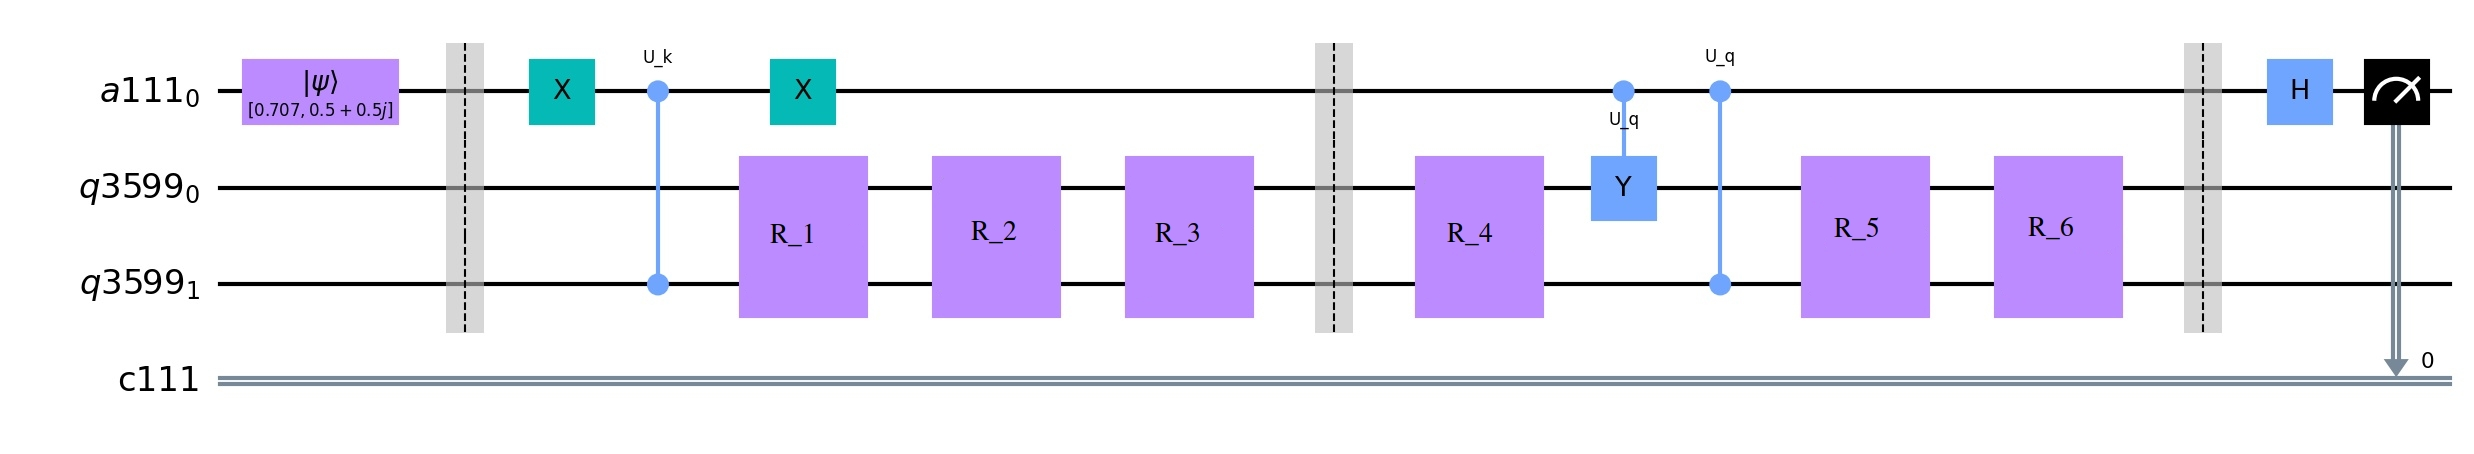
\includegraphics[width=\linewidth]{img/circuit.jpg}
  \caption{Circuit for $k = 1, q = 4, \bm \sigma_{1, iz}, \bm \sigma_{4, yi}, \elec = 2, \orb = 4$}
  \label{fig:circuit}
\end{figure}

With equations for the wavefunction in hand, a circuit can be built to obtain matrices $\bm M$ and $\bm V$ needed to solve the system of Euler-Lagrange equations and accelerate the \gls{tdvp}.

\section{\textbf{Simulation}}

The algorithm was verified via simulating a Quantum Computer. The open-source library Qiskit was used to simulate the \gls{qc} for the algorithm.

\subsection{\textbf{Hardware description}}
The computational experiments were conducted on the Nocona partition at Texas Tech University's High-Performance Computing Center (HPCC). The machines run Linux distro CentOS 8.1, with 240 PowerEdge C6252 nodes and 2 AMD EPYC™ 7702 processors per node.
%

\subsection{\textbf{Simulation and verification}}

The theoretical algebraic derivations for the analytical expressions of the system were obtained so that the could verify the results obtained by our algorithm.
The algorithm calculated the elements $M_{kq}$ and $V_k$ used by the \gls{tdvp} in Eq. \ref{eq:matrixderiv}. The error was then calculated using the Frobenius Norm of the difference between the simulated matrices $\hat {\bm M}$ and $\hat {\bm V}$ and their expected analytical expressions $\bm {\bar M}$ and $\bm {\bar V}$:
%
\begin{equation*}
	\begin{split}
		E_M &= \sqrt{\sum_k \sum_q \lvert {\hat M_{kq} - \bar M_{kq}} \rvert ^ 2 }\\
		E_V &= \sqrt{\sum_k \lvert {\hat V_{k} - \bar V_{k}} \rvert ^ 2 }\\
	\end{split}
\end{equation*}
%
\begin{figure}[h!]
	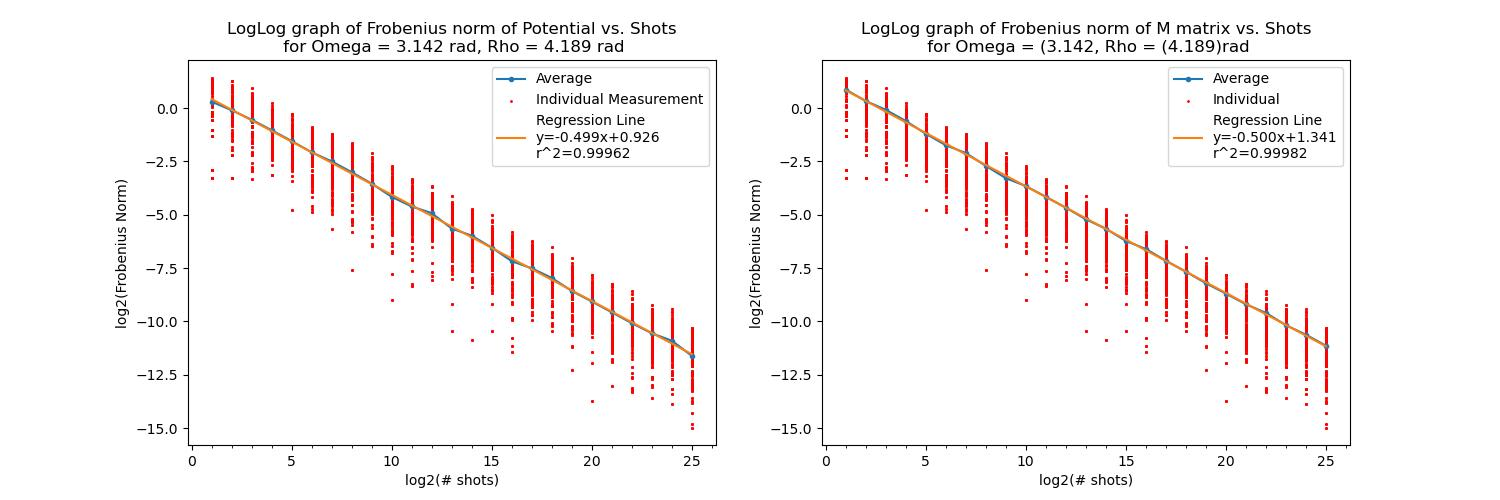
\includegraphics[width=\linewidth]{img/1e.jpg}
  \caption{Loglog graph of error vs number of shots for a hydrogen atom}
  \label{fig:1derrorgraph}
\end{figure}

\begin{figure}[h!]
	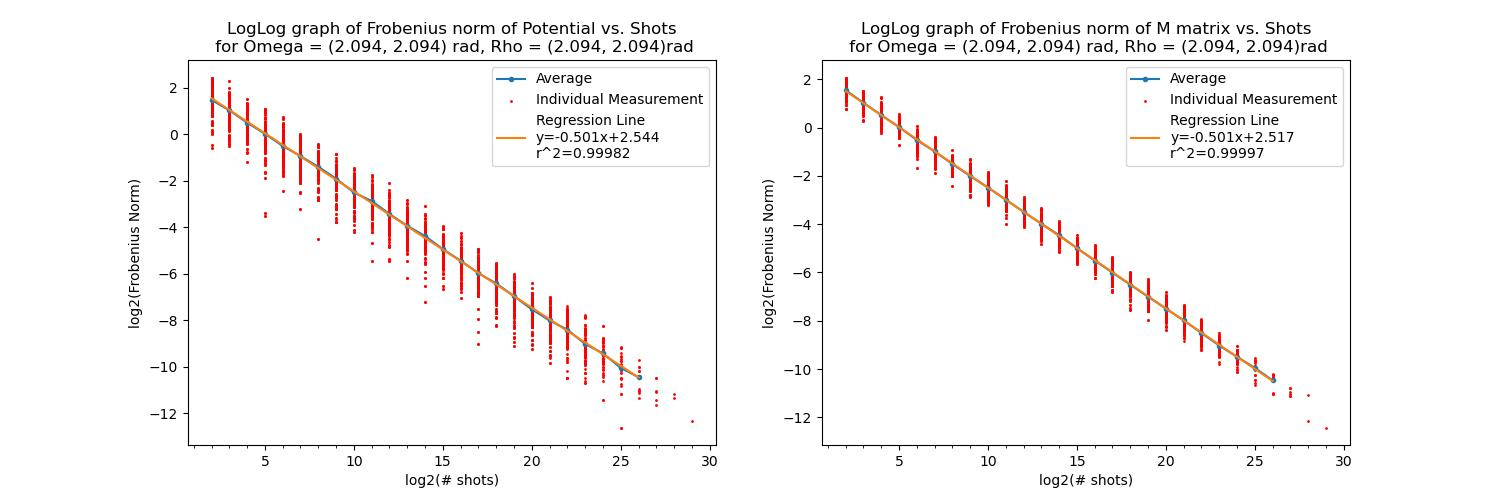
\includegraphics[width=\linewidth]{img/2e-nonint.jpg}
  \caption{Loglog graph of error vs number of shots for a hydrogen molecule}
  \label{fig:2derrorgraph}
\end{figure}

We've plotted the average and individual errors when using $2^S$ shots in the circuits, with $S \in \{1, 2, \ldots, 29\}$. That is, we have results for up to half a billion shots. For most of these values of $S$, the averages had 100 individual experiments run, and we didn't include averages when the number of individual experiments were over 10. The $r^2$ value was calculated over the first-order regression of these averages.
Current results in our simulations of a hydrogen atom as well as a hydrogen molecule suggest that the error $E$ in the approximation for the elements of both the potential matrix $\bm V$ and the matrix $\bm M$ follow the same relationship with the number of shots $S$ in the circuits, as seen in \ref{fig:2derrorgraph}. 
%
\begin{equation*}
	\begin{split}
		\log E &\approx -\frac 1 2 \log S + C \\
		E &\approx \frac 1 {\sqrt{S}} \cdot C' \\
	\end{split}
\end{equation*}
%
Which means the assymptotical behaviour of our error is $\mathcal O(S^{-\frac 1 2})$.

\subsection{\textbf{Conclusion}}

We have proposed the use of Fukutome's \shortcite{fukutome} unitary approach to \gls{hf} theory as a means to obtain an unitary representation for a trial wavefunction, which is necessary for \gls{qc}.
Through some further assumptions and approximations, we've managed to simplify the trial wavefunction so as to be able to use it on a modified circuit inspired by Li's \shortcite{benjamin} work. The circuit remains shallow and error-resistant, allowing its application using today's \gls{nisq} devices.
Thus, we are able to find approximations of matrices $\bm M$ and $\bm V$ that arise from the Euler-Lagrange Eqs. \ref{eq:matrixderiv}.
This approach has netted us a result that requires a number of shots scaling quadratically with the required precision, making it possible to run this quantum circuit as a \gls{nisq} coprocessor to an iterative algorithm, such as the \gls{tdvp}, as expressed in Fig.\ref{fig:TDVP}.
The quantum algorithm calculates matrices $\bm M$ and $\bm V$ and, using this data, a classical computer can solve the differential equations to supply the quantum computer with a new trial wavefunction via the parameter list $\bm \lambda$.

The \gls{tdvp} can then be used in several techniques such as \gls{end}, \gls{slend} or \gls{mcend} to simulate several chemical reactions important in cancer treatment \shortcite{moraleswater,moralesdna,end24,end31,end34}, atmospheric reactions \shortcite{end22,end25,end26,end27,end30,end35} and other applications.

Further research could be made using the non-unitary representation for $\hat U$ in combination with \gls{lcu} to allow for \gls{qc} in the non-unitary case or even different formulations for the wavefunction in place of \gls{hf}.
Other directions of study would be to apply the technique to simulate reactions with polymers and organic tissue or reactions in crystals, both of which would have geometric features that would allow us to apply this technique.
%%%%%%%%%%%%%%%%%%%%%%%%%%%%%%%%%%%%%%%%%%%%%%
%Backmatter -- Bibliography, appendices, etc.%
%%%%%%%%%%%%%%%%%%%%%%%%%%%%%%%%%%%%%%%%%%%%%%
\backmatter


%%%%%%%%%%%%%%%%%%%%%%%%%%%%%%%%%%%%%%%%%%%%%%%%%%%%%%%%
%Bibliography:  Use BibTeX 							   %
%%%%%%%%%%%%%%%%%%%%%%%%%%%%%%%%%%%%%%%%%%%%%%%%%%%%%%%%
\bibliographystyle{chicago}
\addcontentsline{toc}{chapter}{\textbf{References}}
\bibliography{aux/refs}

\glsaddall

%\setlength{\glsdescwidth}{0.5\linewidth}
%\setlength{\glspagelistwidth}{0.1\linewidth}
\printnoidxglossary[type=acronym,sort=letter]
%\printnoidxglossary[type=symbols,sort=letter]

\end{document}
